
% LaTeX Beamer file automatically generated from DocOnce
% https://github.com/doconce/doconce

%-------------------- begin beamer-specific preamble ----------------------

\documentclass{beamer}

\usetheme{red_plain}
\usecolortheme{default}

% turn off the almost invisible, yet disturbing, navigation symbols:
\setbeamertemplate{navigation symbols}{}

% Examples on customization:
%\usecolortheme[named=RawSienna]{structure}
%\usetheme[height=7mm]{Rochester}
%\setbeamerfont{frametitle}{family=\rmfamily,shape=\itshape}
%\setbeamertemplate{items}[ball]
%\setbeamertemplate{blocks}[rounded][shadow=true]
%\useoutertheme{infolines}
%
%\usefonttheme{}
%\useinntertheme{}
%
%\setbeameroption{show notes}
%\setbeameroption{show notes on second screen=right}

% fine for B/W printing:
%\usecolortheme{seahorse}

\usepackage{pgf}
\usepackage{graphicx}
\usepackage{epsfig}
\usepackage{relsize}

\usepackage{fancybox}  % make sure fancybox is loaded before fancyvrb

\usepackage{fancyvrb}
%\usepackage{minted} % requires pygments and latex -shell-escape filename
%\usepackage{anslistings}
%\usepackage{listingsutf8}

\usepackage{amsmath,amssymb,bm}
%\usepackage[latin1]{inputenc}
\usepackage[T1]{fontenc}
\usepackage[utf8]{inputenc}
\usepackage{colortbl}
\usepackage[english]{babel}
\usepackage{tikz}
\usepackage{framed}
% Use some nice templates
\beamertemplatetransparentcovereddynamic

% --- begin table of contents based on sections ---
% Delete this, if you do not want the table of contents to pop up at
% the beginning of each section:
% (Only section headings can enter the table of contents in Beamer
% slides generated from DocOnce source, while subsections are used
% for the title in ordinary slides.)
\AtBeginSection[]
{
  \begin{frame}<beamer>[plain]
  \frametitle{}
  %\frametitle{Outline}
  \tableofcontents[currentsection]
  \end{frame}
}
% --- end table of contents based on sections ---

% If you wish to uncover everything in a step-wise fashion, uncomment
% the following command:

%\beamerdefaultoverlayspecification{<+->}

\newcommand{\shortinlinecomment}[3]{\note{\textbf{#1}: #2}}
\newcommand{\longinlinecomment}[3]{\shortinlinecomment{#1}{#2}{#3}}

\definecolor{linkcolor}{rgb}{0,0,0.4}
\hypersetup{
    colorlinks=true,
    linkcolor=linkcolor,
    urlcolor=linkcolor,
    pdfmenubar=true,
    pdftoolbar=true,
    bookmarksdepth=3
    }
\setlength{\parskip}{0pt}  % {1em}

\newenvironment{doconceexercise}{}{}
\newcounter{doconceexercisecounter}
\newenvironment{doconce:movie}{}{}
\newcounter{doconce:movie:counter}

\newcommand{\subex}[1]{\noindent\textbf{#1}}  % for subexercises: a), b), etc

%-------------------- end beamer-specific preamble ----------------------

% Add user's preamble




% insert custom LaTeX commands...

\raggedbottom
\makeindex

%-------------------- end preamble ----------------------

\begin{document}

% matching end for #ifdef PREAMBLE

\newcommand{\exercisesection}[1]{\subsection*{#1}}



% ------------------- main content ----------------------



% ----------------- title -------------------------

\title{Thirty Years of Education and Research on Nuclear Many-Body Physics at the ECT*; from traditional Methods to Quantum Computing and Machine Learning}

% ----------------- author(s) -------------------------

\author{Morten Hjorth-Jensen\inst{1}}
\institute{Department of Physics and Astronomy and FRIB, Michigan State University, USA, and Department of Physics and Center for Computing in Science Education, University of Oslo, Norway\inst{1}}
% ----------------- end author(s) -------------------------

\date{30th anniversary ECT*, October 4, 2023
% <optional titlepage figure>
% <optional copyright>
}

\begin{frame}[plain,fragile]
\titlepage
\end{frame}

\begin{frame}[plain,fragile]
\frametitle{What is this talk about?}

\begin{block}{}
The main emphasis is to give you a short and pedestrian introduction to the whys and hows we can use (with several examples) machine learning methods
in nuclear physics. And why this could (or should) be of interest. And how this can be linked with standard many-body theories. And perhaps some quantum computing.
\end{block}

\begin{block}{}
I will also try to highlight educational initiatives and strategies where the ECT* has played and will/can play an important role in educating the next generation of nuclear scientists
\end{block}

\begin{block}{Additional info }
Parts of this talk are based on \href{{https://journals.aps.org/rmp/abstract/10.1103/RevModPhys.94.031003}}{Artificial Intelligence and Machine Learning in Nuclear Physics, Amber Boehnlein et al., Reviews Modern of Physics 94, 031003 (2022)} 

\end{block}
\end{frame}

\begin{frame}[plain,fragile]
\frametitle{Thanks to many}

Jane Kim (MSU), Julie Butler (MSU), Patrick Cook (MSU), Danny Jammooa (MSU), Daniel Bazin (MSU), Dean Lee (MSU), Witek Nazarewicz (MSU), Michelle Kuchera (Davidson College), Even Nordhagen (UiO), Robert Solli (UiO, Expert Analytics), Bryce Fore (ANL), Alessandro Lovato (ANL), Stefano Gandolfi (LANL), Francesco Pederiva (UniTN), and Giuseppe Carleo (EPFL). 
Niyaz Beysengulov and Johannes Pollanen (experiment, MSU); Zachary Stewart, Jared Weidman, and Angela Wilson (quantum chemistry, MSU)
Jonas Flaten, Oskar, Leinonen, Øyvind Sigmundson Schøyen, Stian Dysthe Bilek, and Håkon Emil Kristiansen (UiO). Marianne Bathen and Lasse Vines (experiments (UiO). Excuses to those I have omitted.
\end{frame}

\begin{frame}[plain,fragile]
\frametitle{The first postdocs and long-term visitors, 1994-1996}

\begin{itemize}
\item Two Brazilians professors on sabbatical leave, \href{{https://www.if.ufrj.br/en/docentes/marta-feijo-barroso/}}{Marta F.~Barroso} and \href{{https://www.if.ufrj.br/~carlos/carlos.html}}{Carlos Aguiar}; \href{{https://artsandscience.usask.ca/profile/ETomusiak}}{Edward Tomusiak from Canada}

\item \href{{http://www.scl.rs/scl-members/members/28-scl-members/members/413-aleksandar-belic-cv}}{Alexandar Belic}; \href{{http://www.inp.demokritos.gr/staff-members/dennis-bonatsos/}}{Dennis Bonatsos}

\item \href{{https://en.unimib.it/fabio-vittorio-de-blasio}}{Fabio Vittorio De Blasio}; \href{{https://pure.au.dk/portal/en/persons/dmitri-fedorov(9a03b124-d457-419c-b2e6-ca4e686b3b96).html}}{Dima Fedorov}

\item Hilmar Forkel; \href{{https://www.crab.org/research-statisticians.html}}{Antje Hoering}

\item Gianluca Lazzari; \href{{https://www.physik.tu-darmstadt.de/der_fachbereich/lehrende_physik/professor_innen_details_26176.en.jsp}}{Mathias Lutz}

\item \href{{https://www.q-info.org/about-me/}}{Jochen Rau}; MHJ
\end{itemize}

\noindent
\end{frame}

\begin{frame}[plain,fragile]
\frametitle{One of the first many-body workshops, summer 1997}

\vspace{6mm}

% inline figure
\centerline{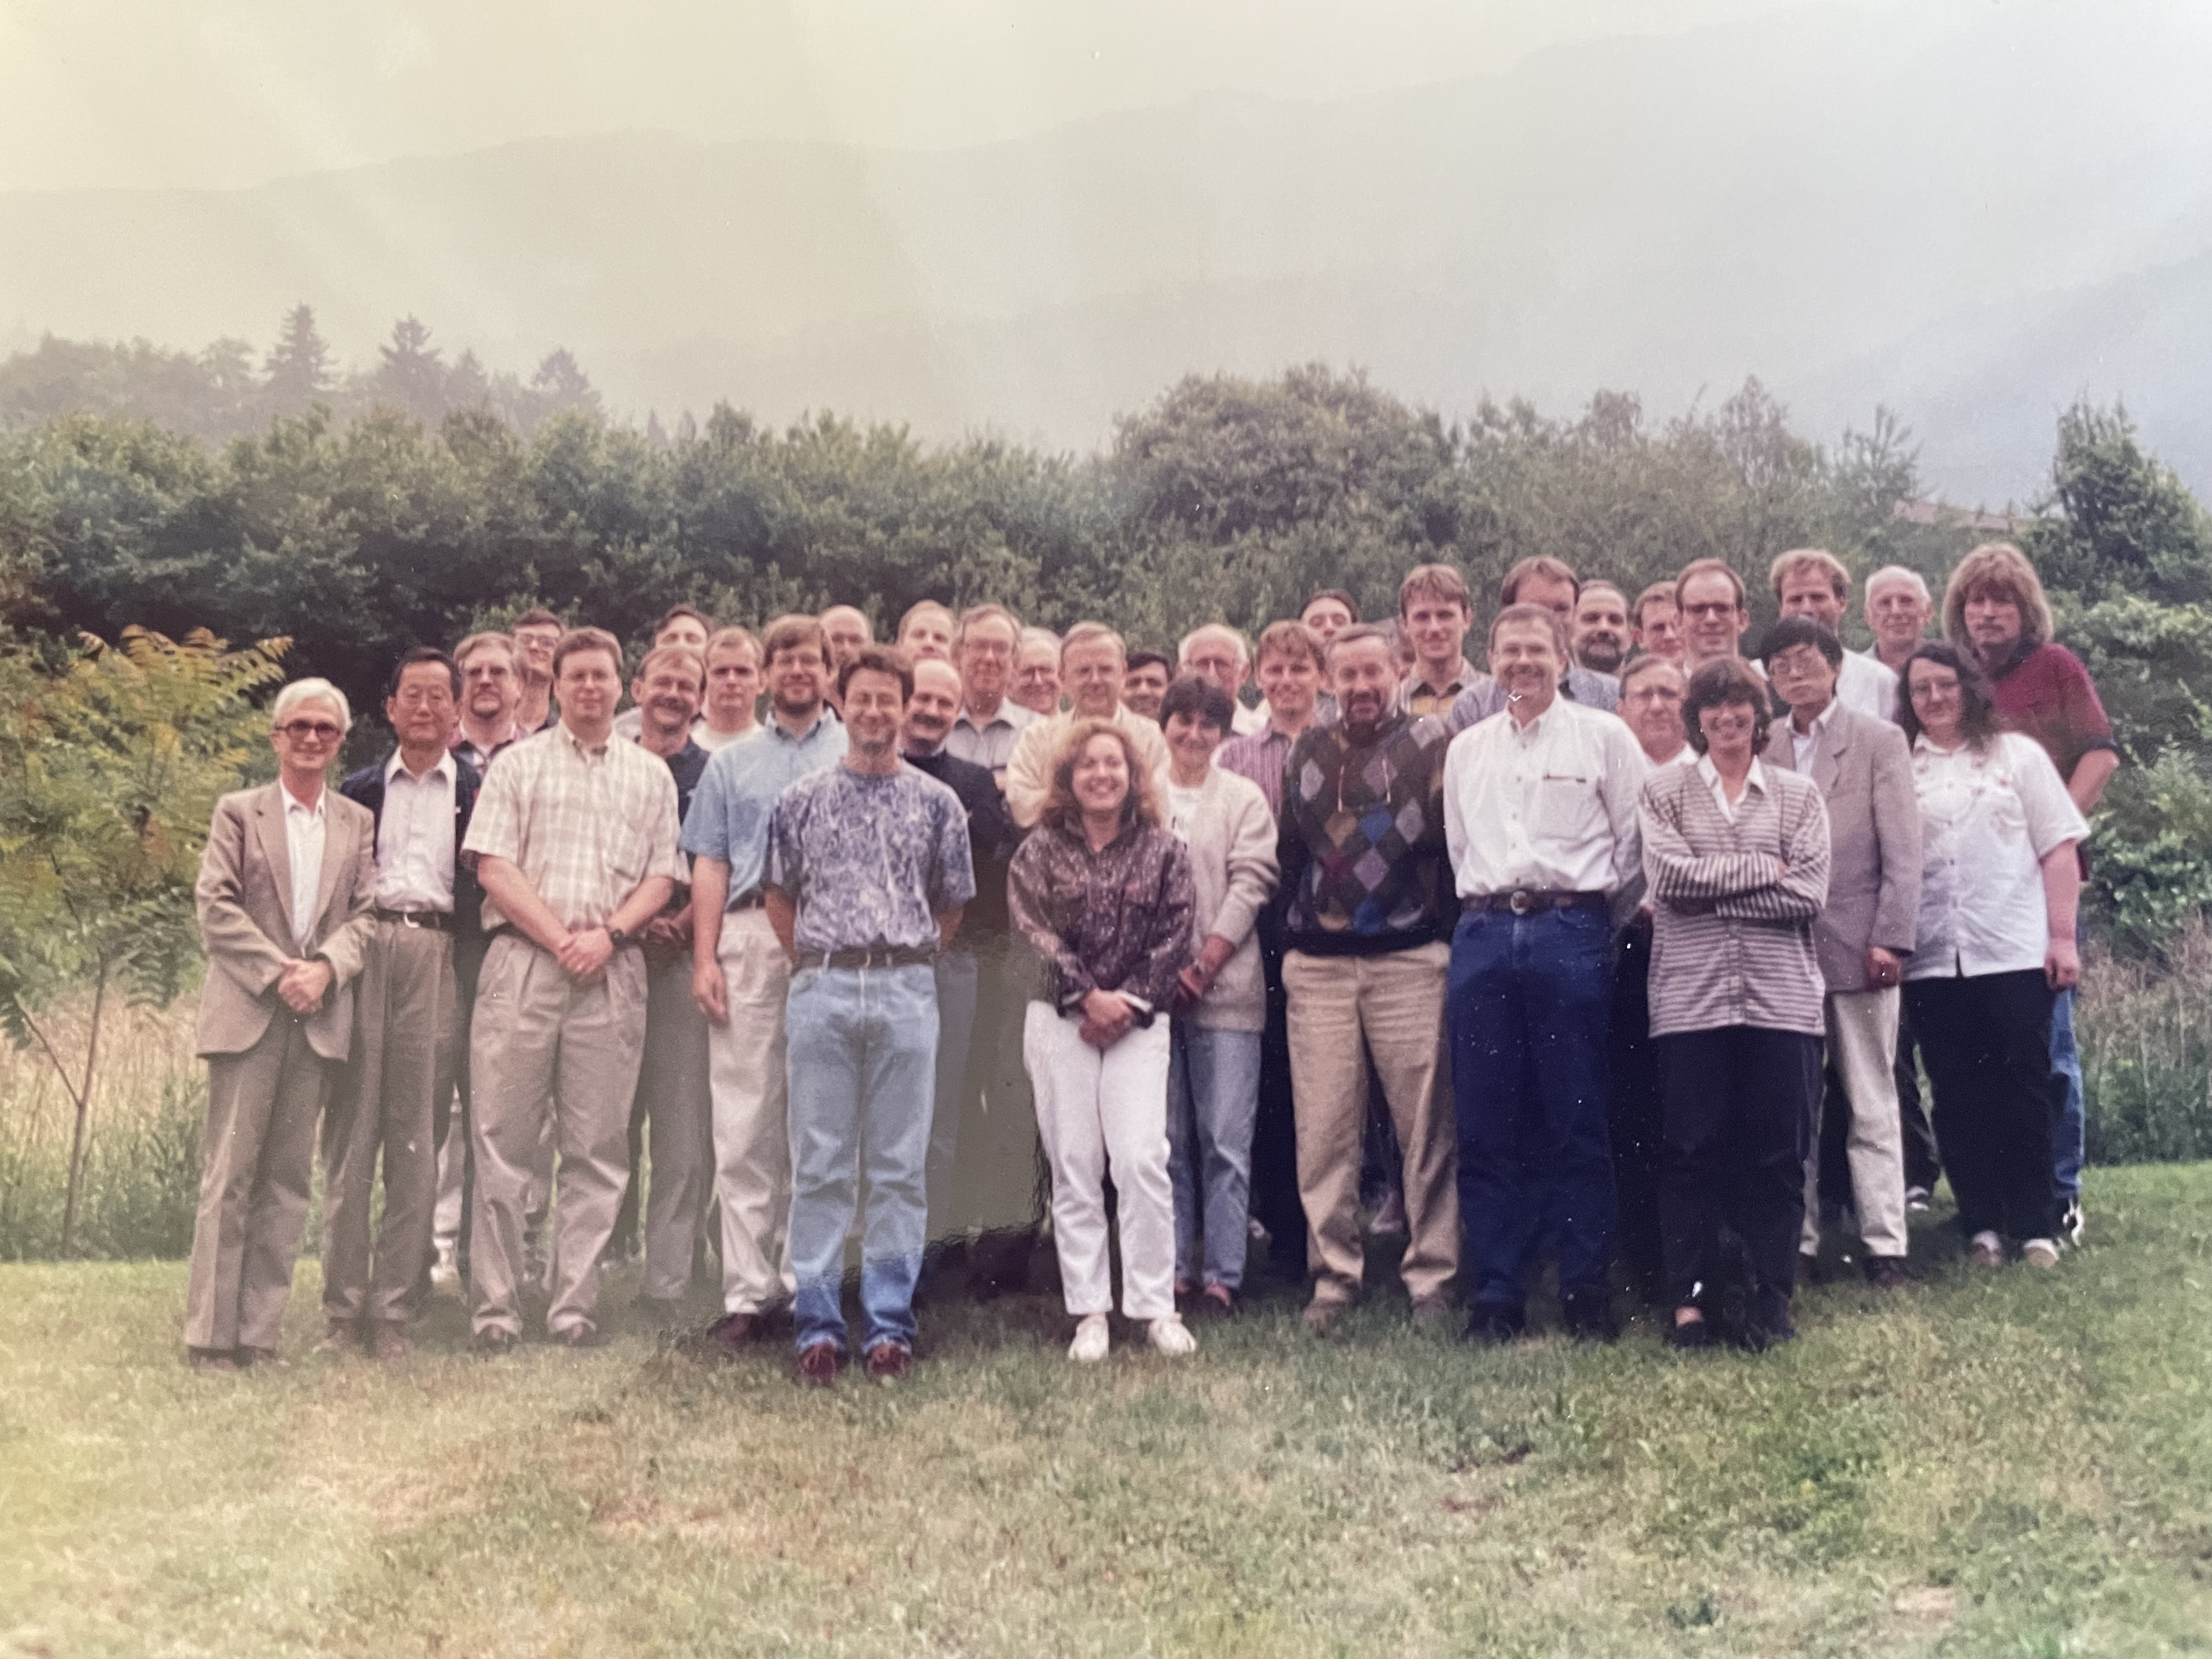
\includegraphics[width=1.0\linewidth]{Photos/manybody1997.jpeg}}

\vspace{6mm}
\end{frame}

\begin{frame}[plain,fragile]
\frametitle{Educational mission and strategic initiatives}

\begin{itemize}
\item \href{{https://www.ectstar.eu/wp-content/uploads/2020/07/annualrep2002.pdf}}{First doctoral training program summer 2002 under the Marie Curie program, Hot and dense QCD}

\item First Nuclear Talent course summer 2012, focus on computational many-body methods, nuclear shell-model and Monte Carlo methods
\end{itemize}

\noindent
\end{frame}

\begin{frame}[plain,fragile]
\frametitle{The Nuclear TALENT initiative}

\href{{https://fribtheoryalliance.org/TALENT/}}{Training in Advanced Low Energy Nuclear Theory},  
aims at providing an advanced and comprehensive training to graduate students
and young researchers in low-energy nuclear theory. The initiative
is a multinational network between several Asian, European and Northern
American institutions and aims at developing a broad curriculum that
will provide the platform for a cutting-edge theory for understanding
nuclei and nuclear reactions.

These objectives are met by
offering series of lectures, commissioned from experienced teachers
in nuclear theory. The educational material generated under this
program will be collected in the form of WEB-based courses,
textbooks, and a variety of modern educational resources. No such
all-encompassing material is available at present; its development
will allow dispersed university groups to profit from the best
expertise available.

The ECT* and the INT have played central roles here.
\end{frame}

\begin{frame}[plain,fragile]
\frametitle{The first ever Nuclear Talent course, ECT*, summer 2012}

\vspace{6mm}

% inline figure
\centerline{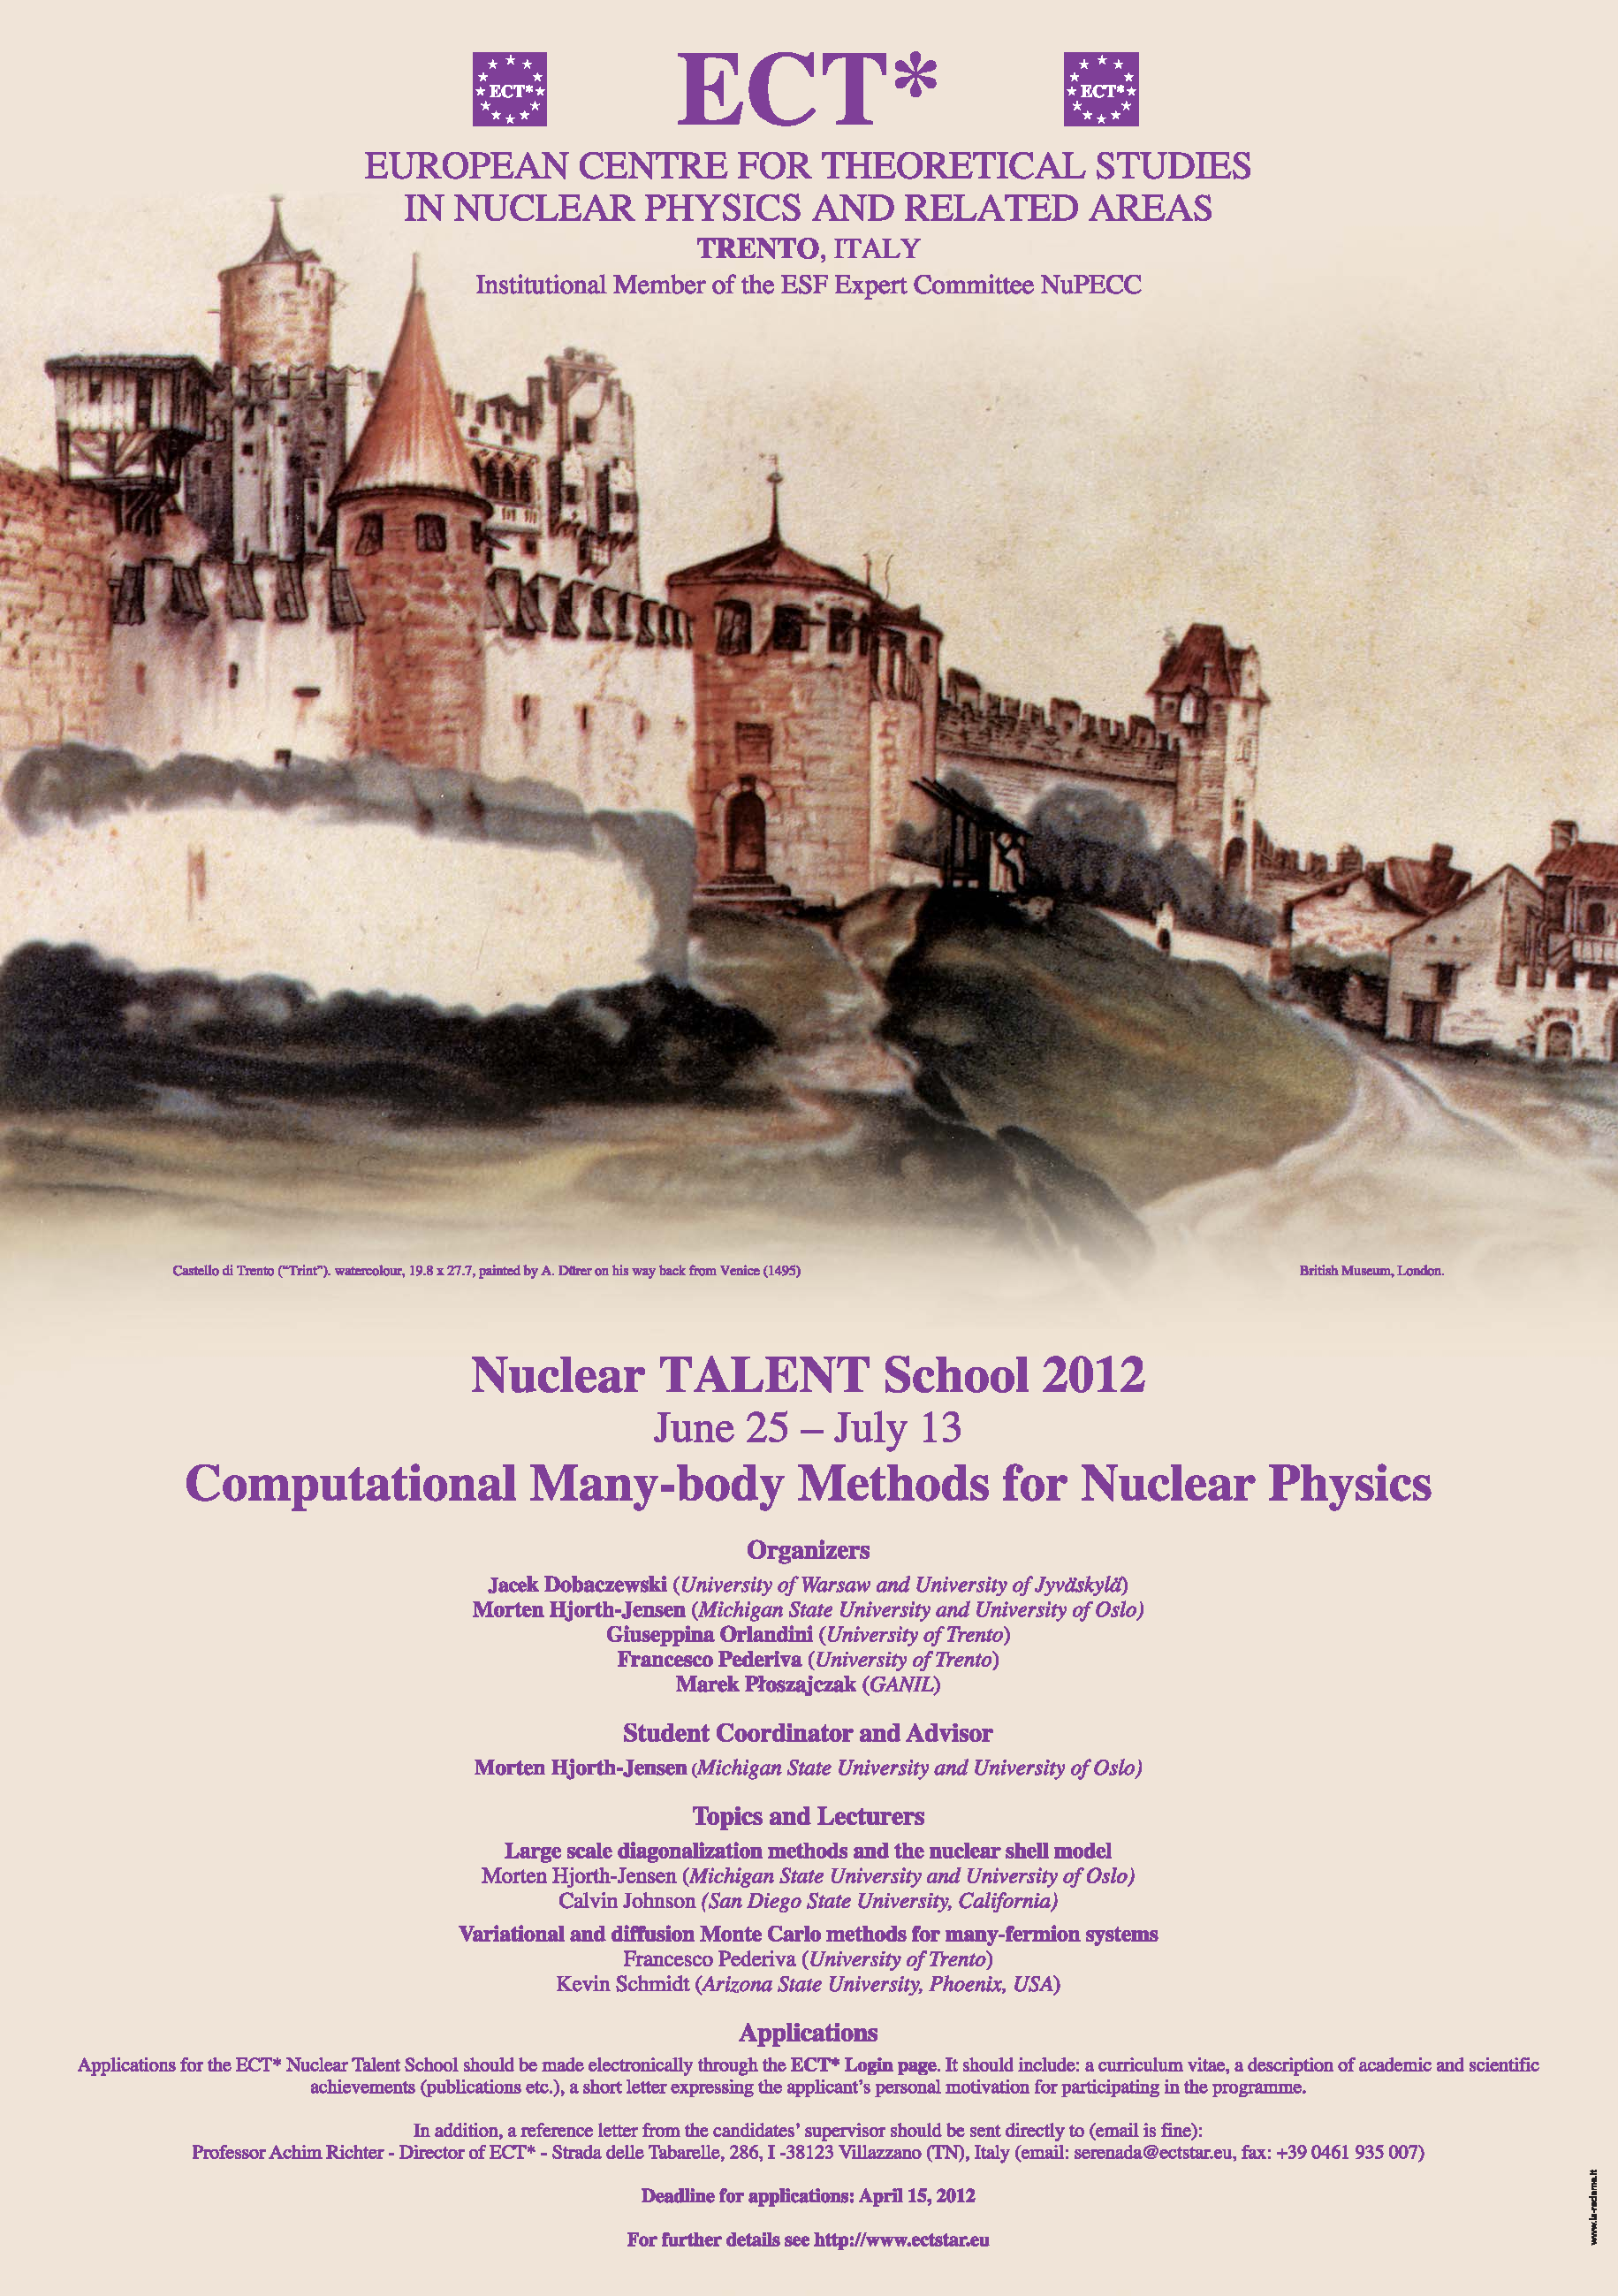
\includegraphics[width=0.6\linewidth]{Photos/talent2012.pdf}}

\vspace{6mm}
\end{frame}

\begin{frame}[plain,fragile]
\frametitle{The second Nuclear Talent course at the ECT*, summer 2014}

\vspace{6mm}

% inline figure
\centerline{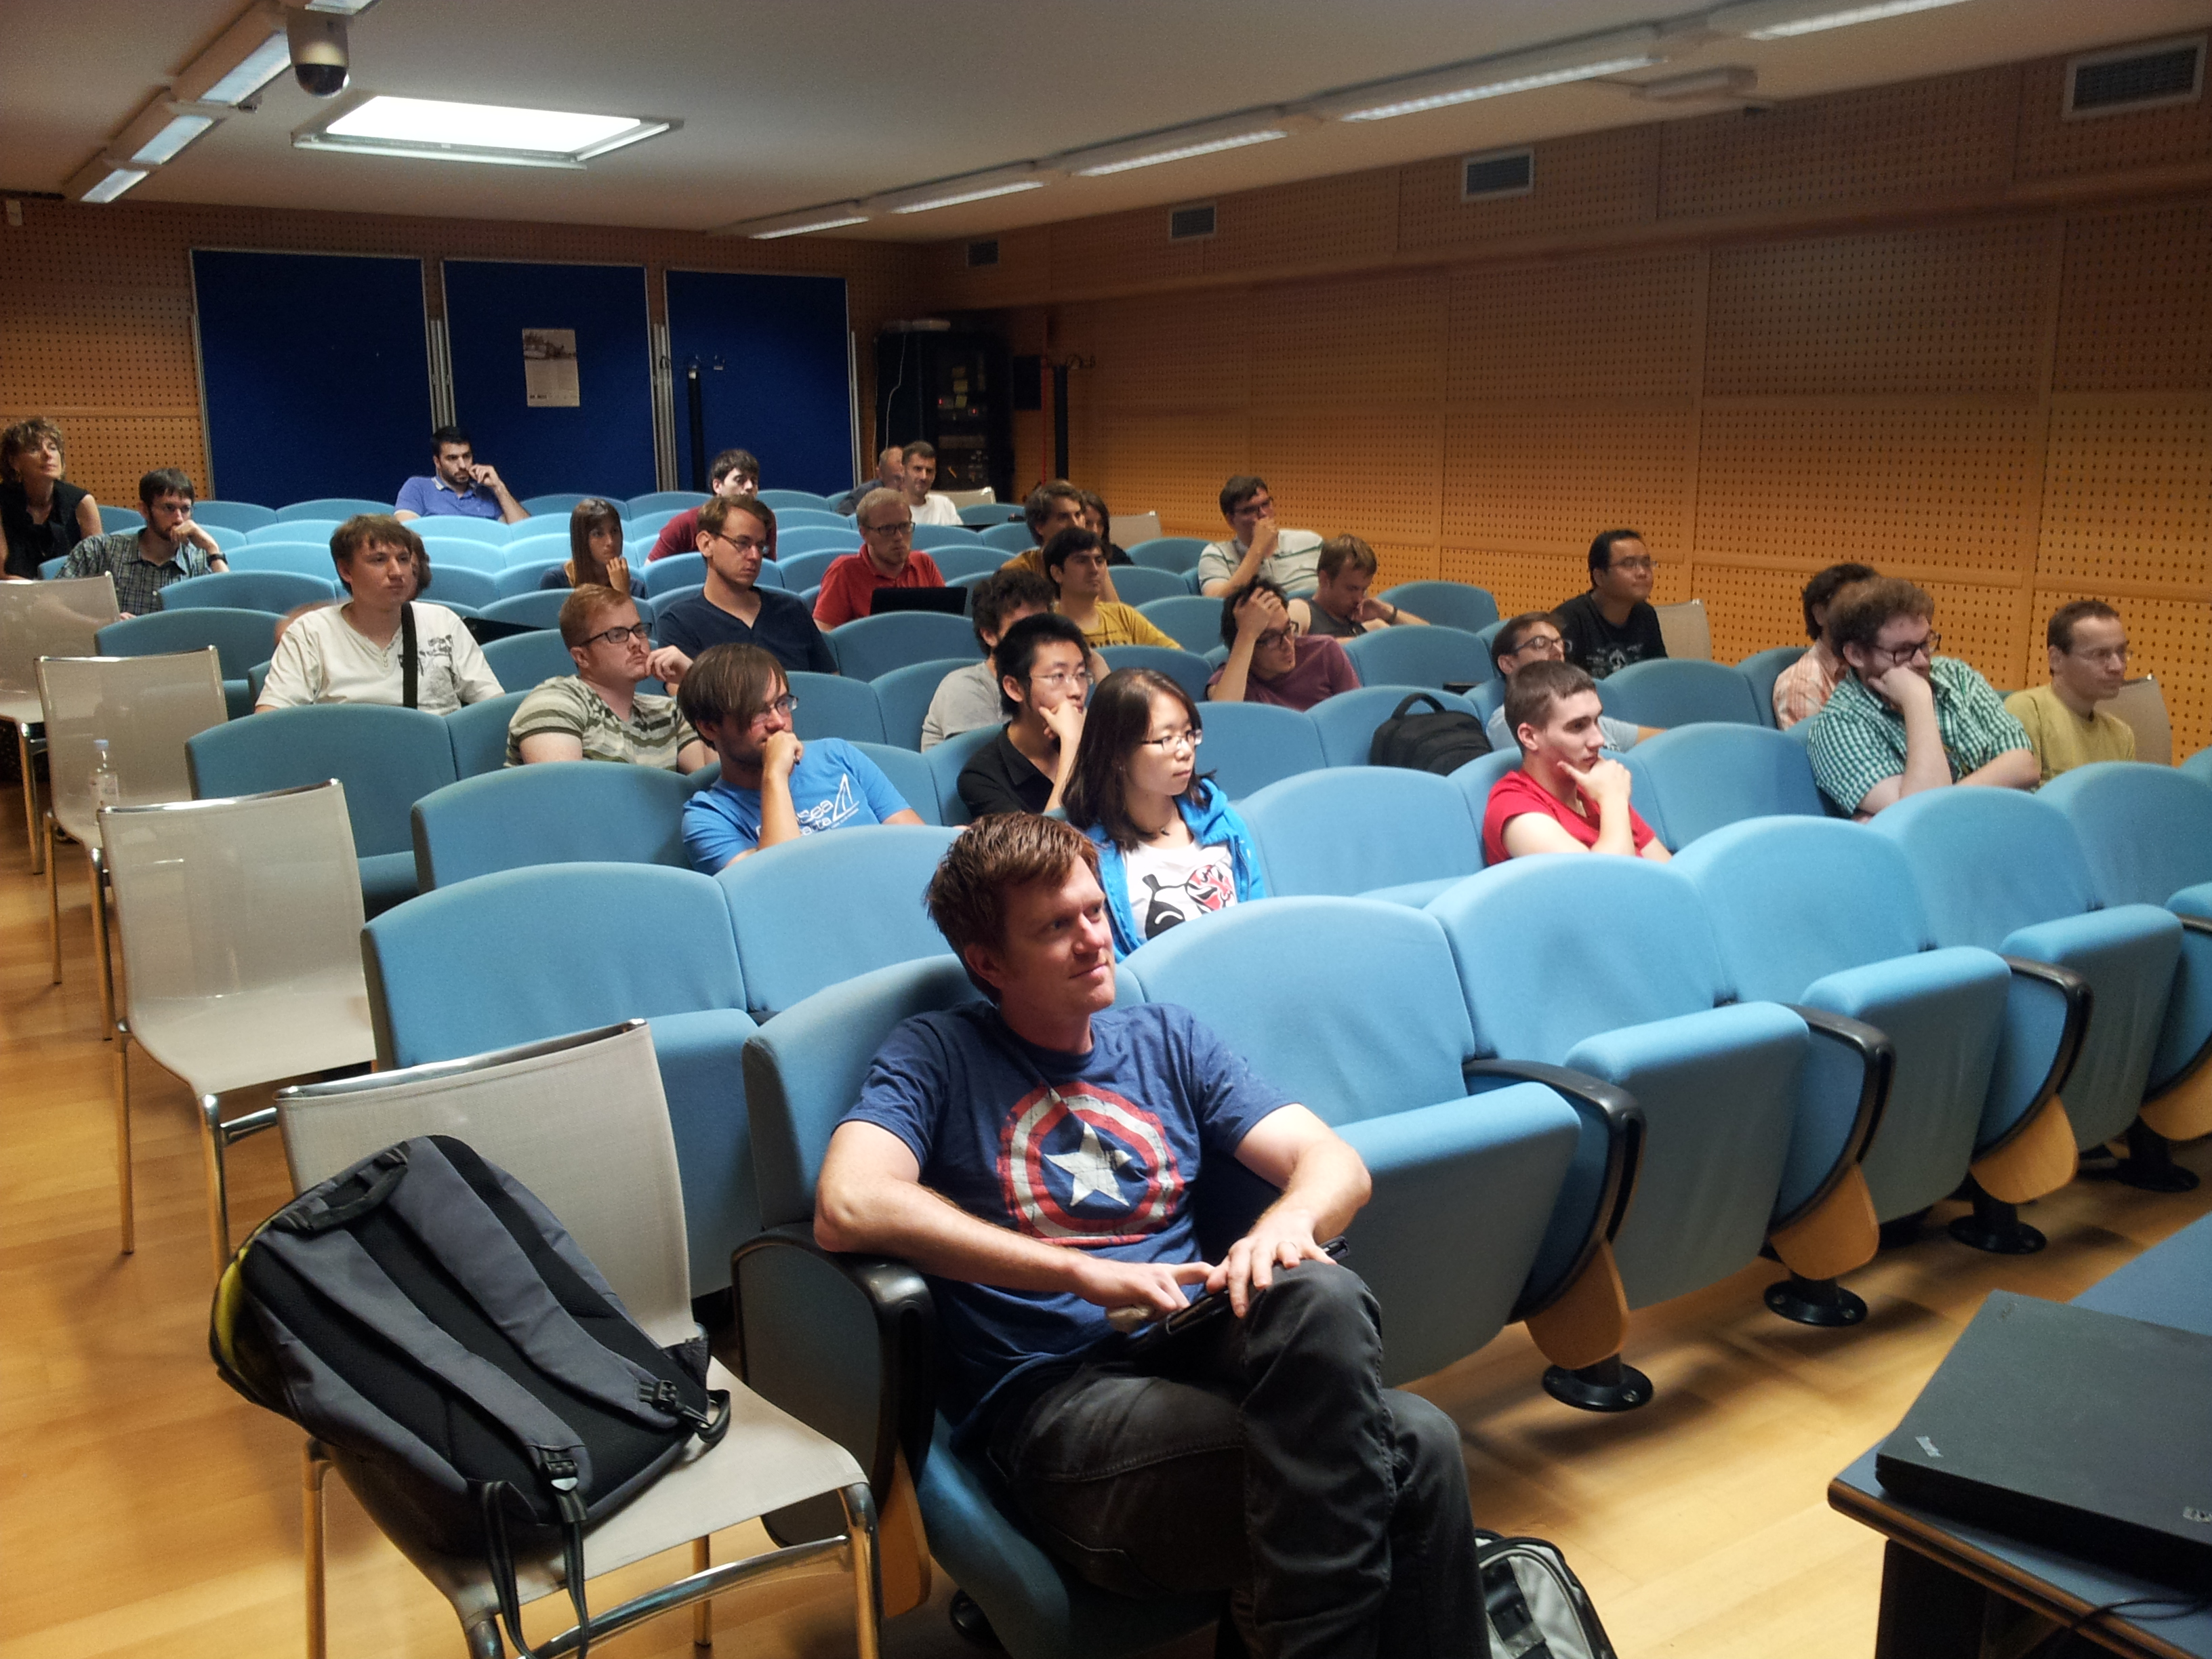
\includegraphics[width=1.0\linewidth]{Photos/talent2014a.jpg}}

\vspace{6mm}
\end{frame}

\begin{frame}[plain,fragile]
\frametitle{The second Nuclear Talent course at the ECT*, summer 2014}

\vspace{6mm}

% inline figure
\centerline{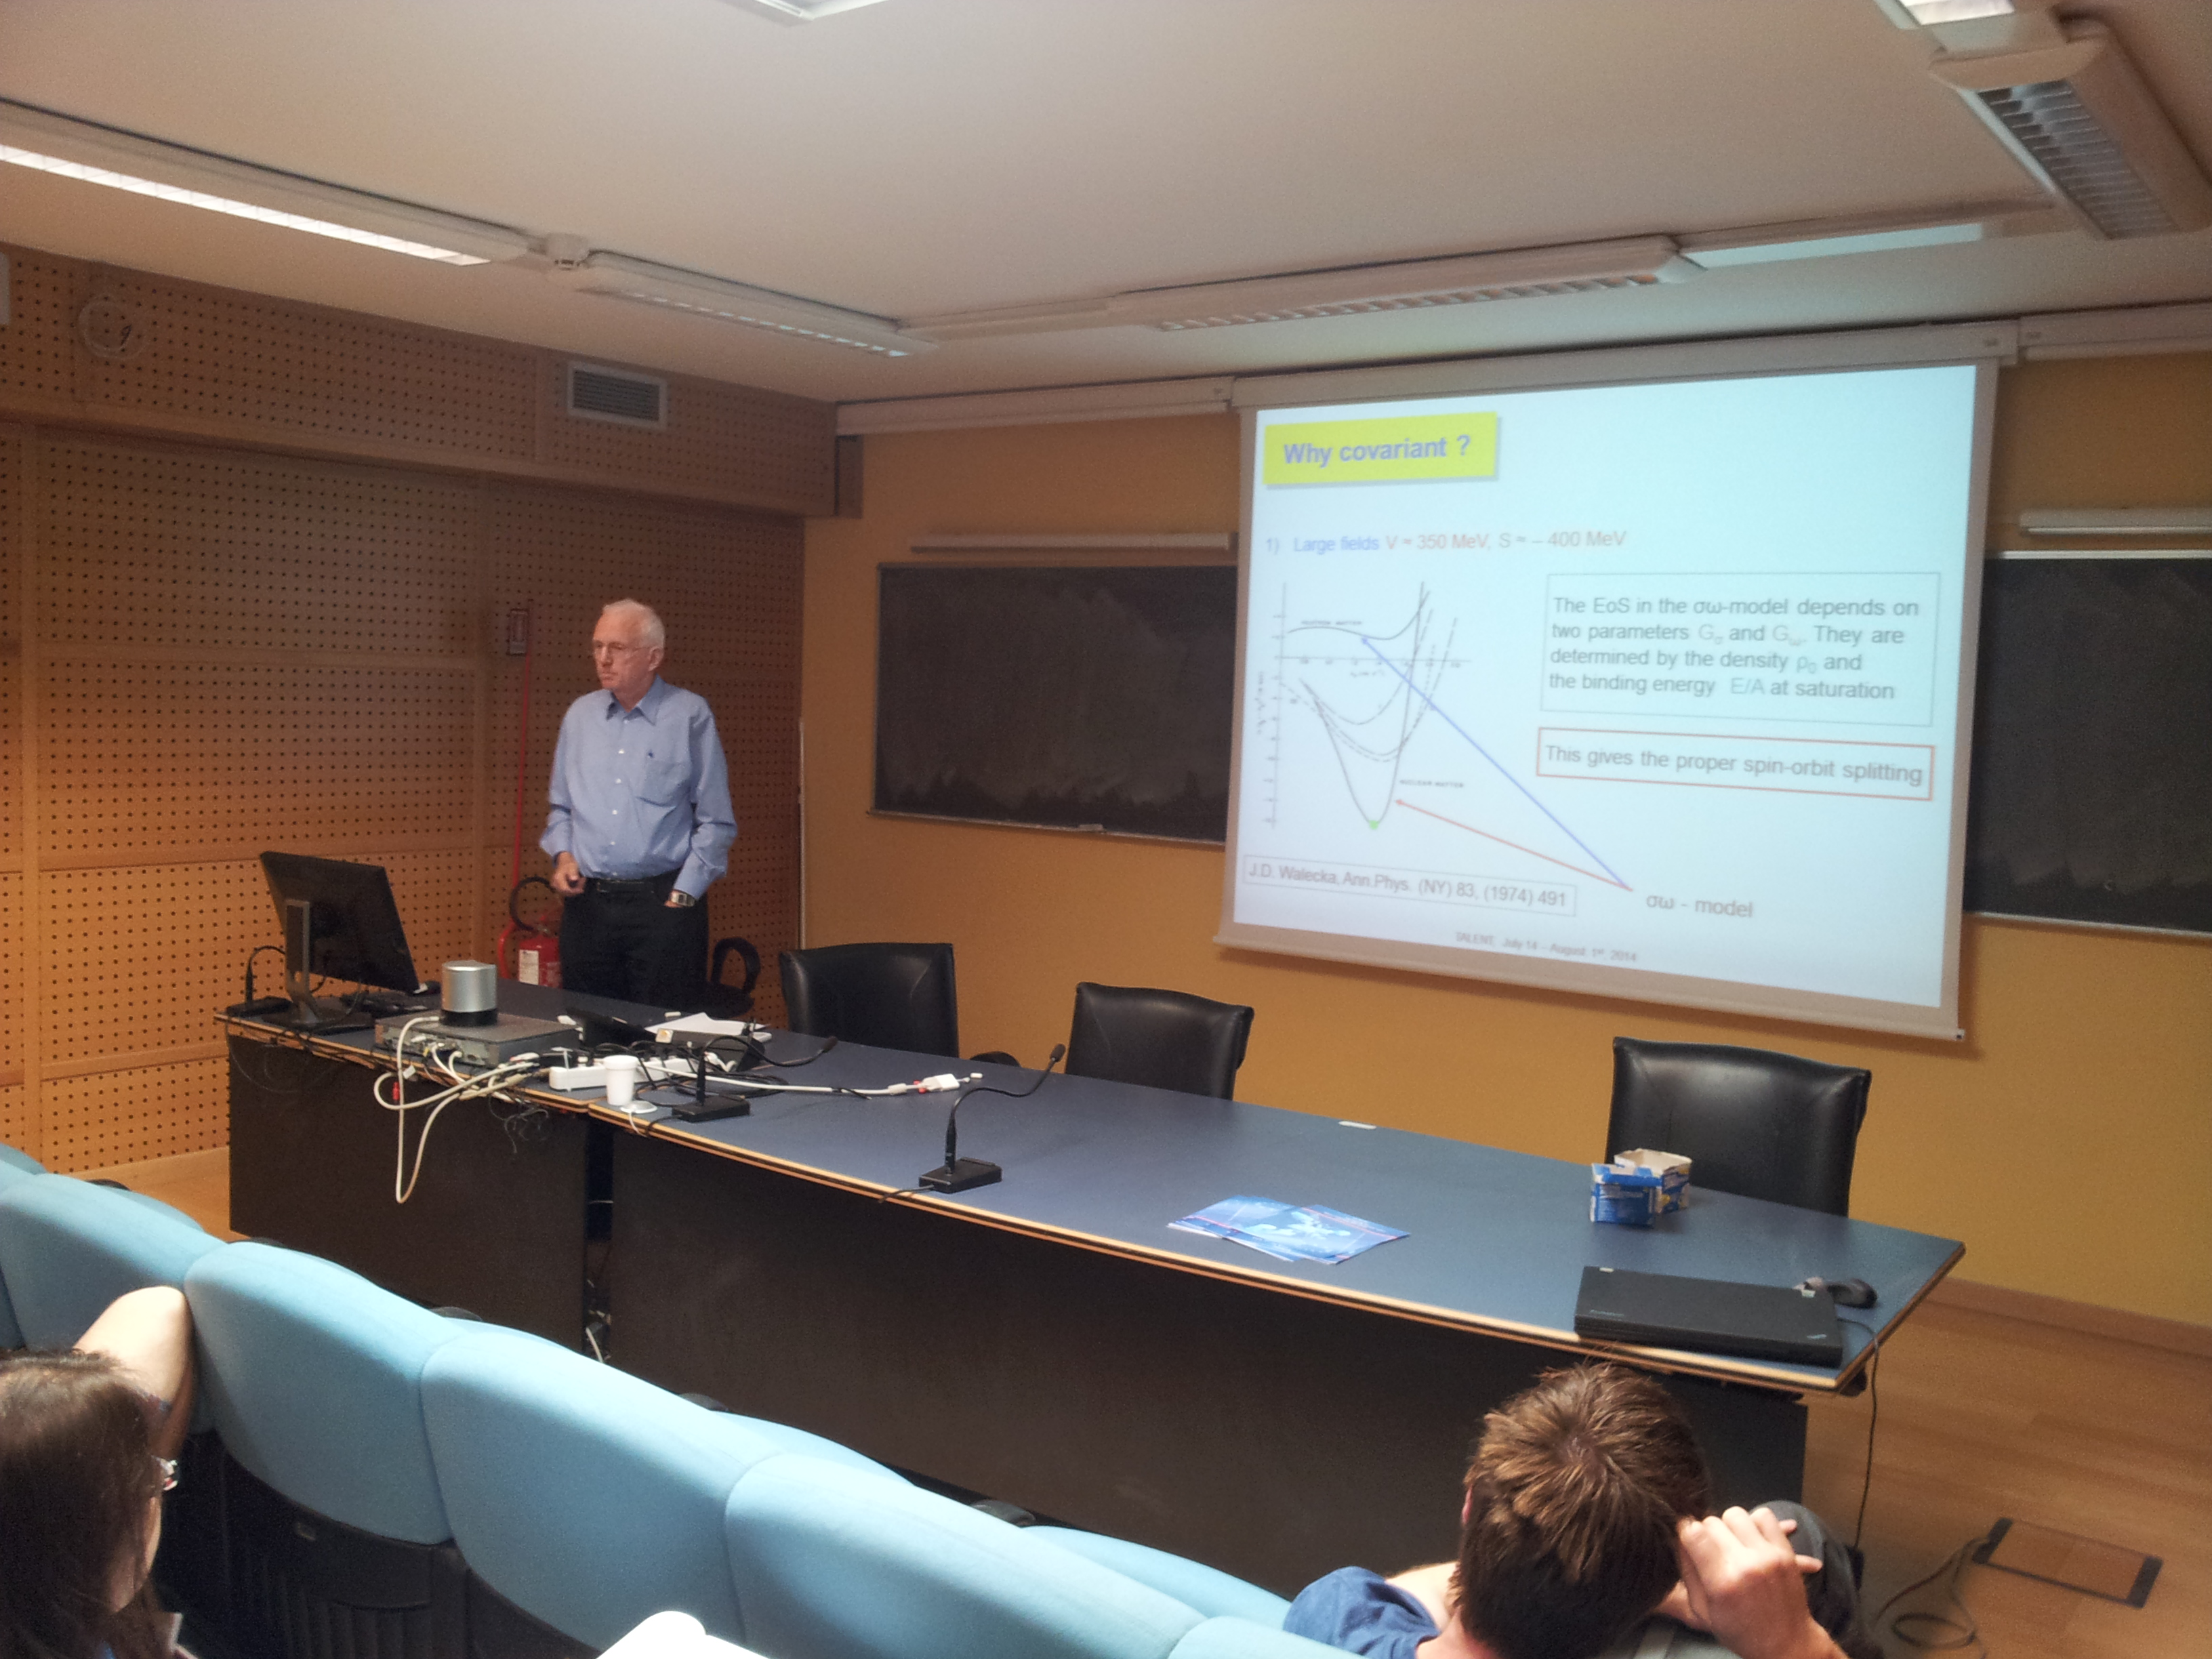
\includegraphics[width=1.0\linewidth]{Photos/talent2014b.jpg}}

\vspace{6mm}
\end{frame}

\begin{frame}[plain,fragile]
\frametitle{Nuclear Talent course summer 2017}

\vspace{6mm}

% inline figure
\centerline{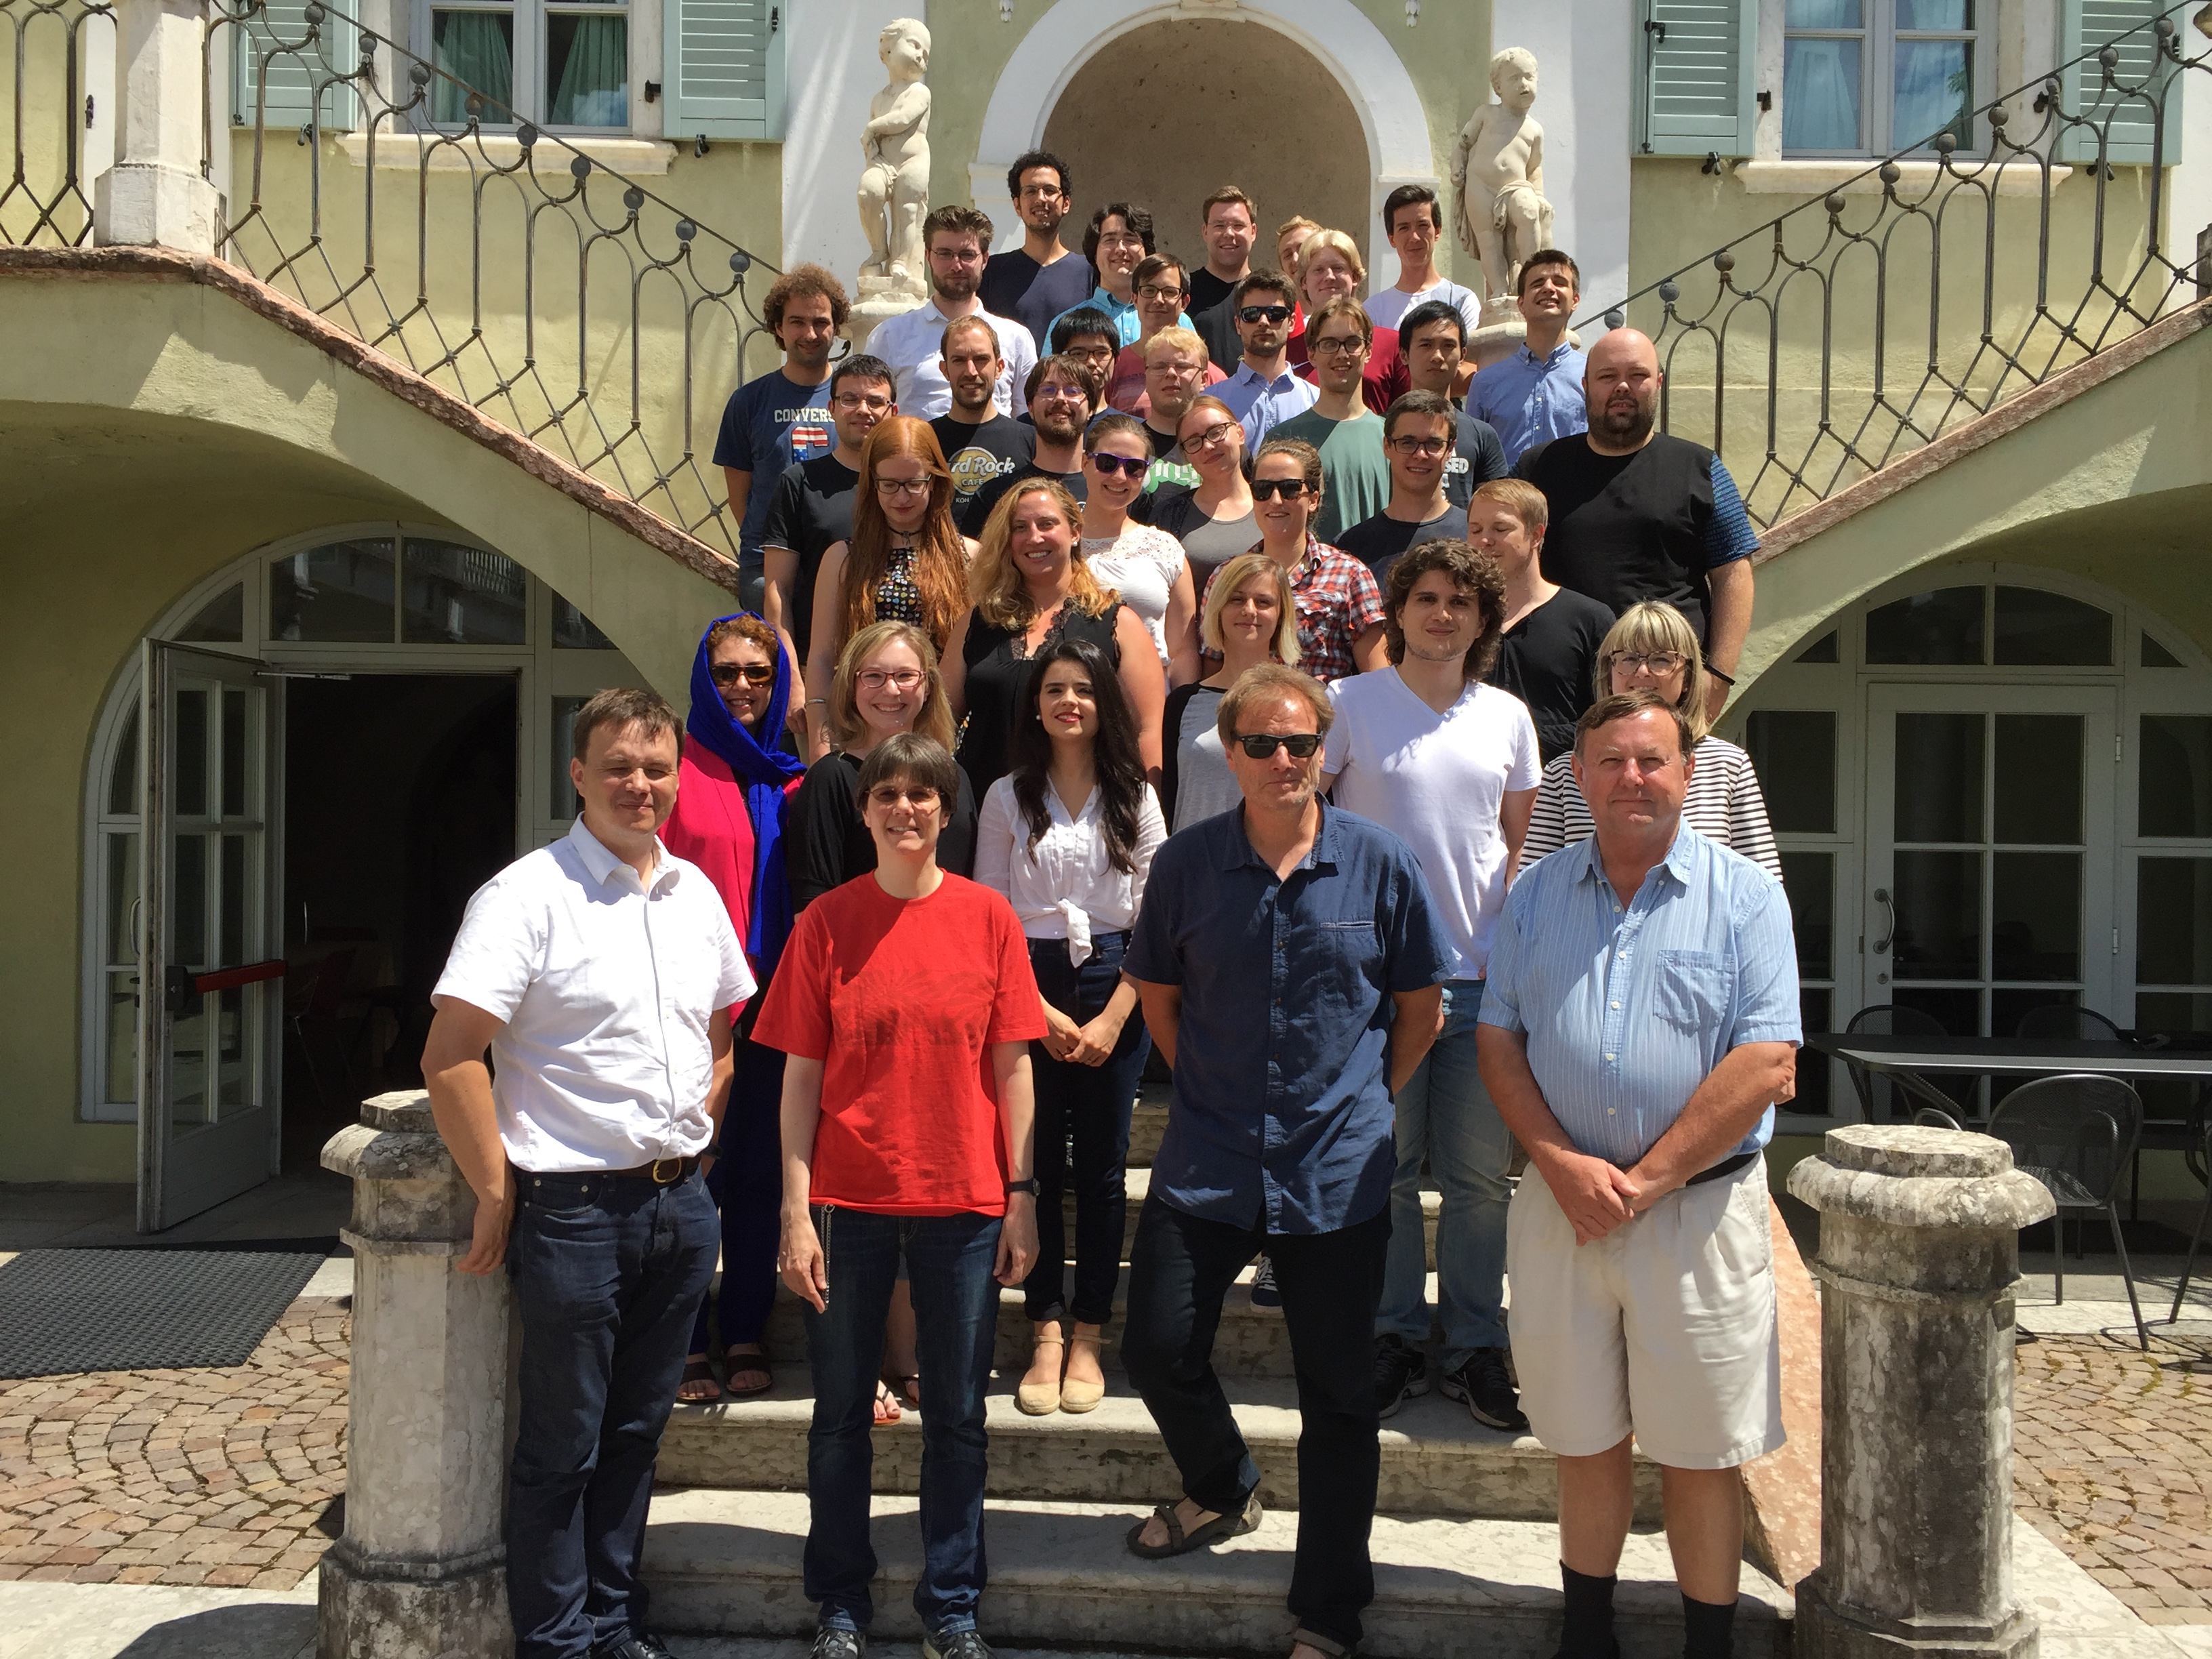
\includegraphics[width=1.0\linewidth]{Photos/talent2017.jpg}}

\vspace{6mm}
\end{frame}

\begin{frame}[plain,fragile]
\frametitle{Nuclear Talent course summer 2018 in China}

\vspace{6mm}

% inline figure
\centerline{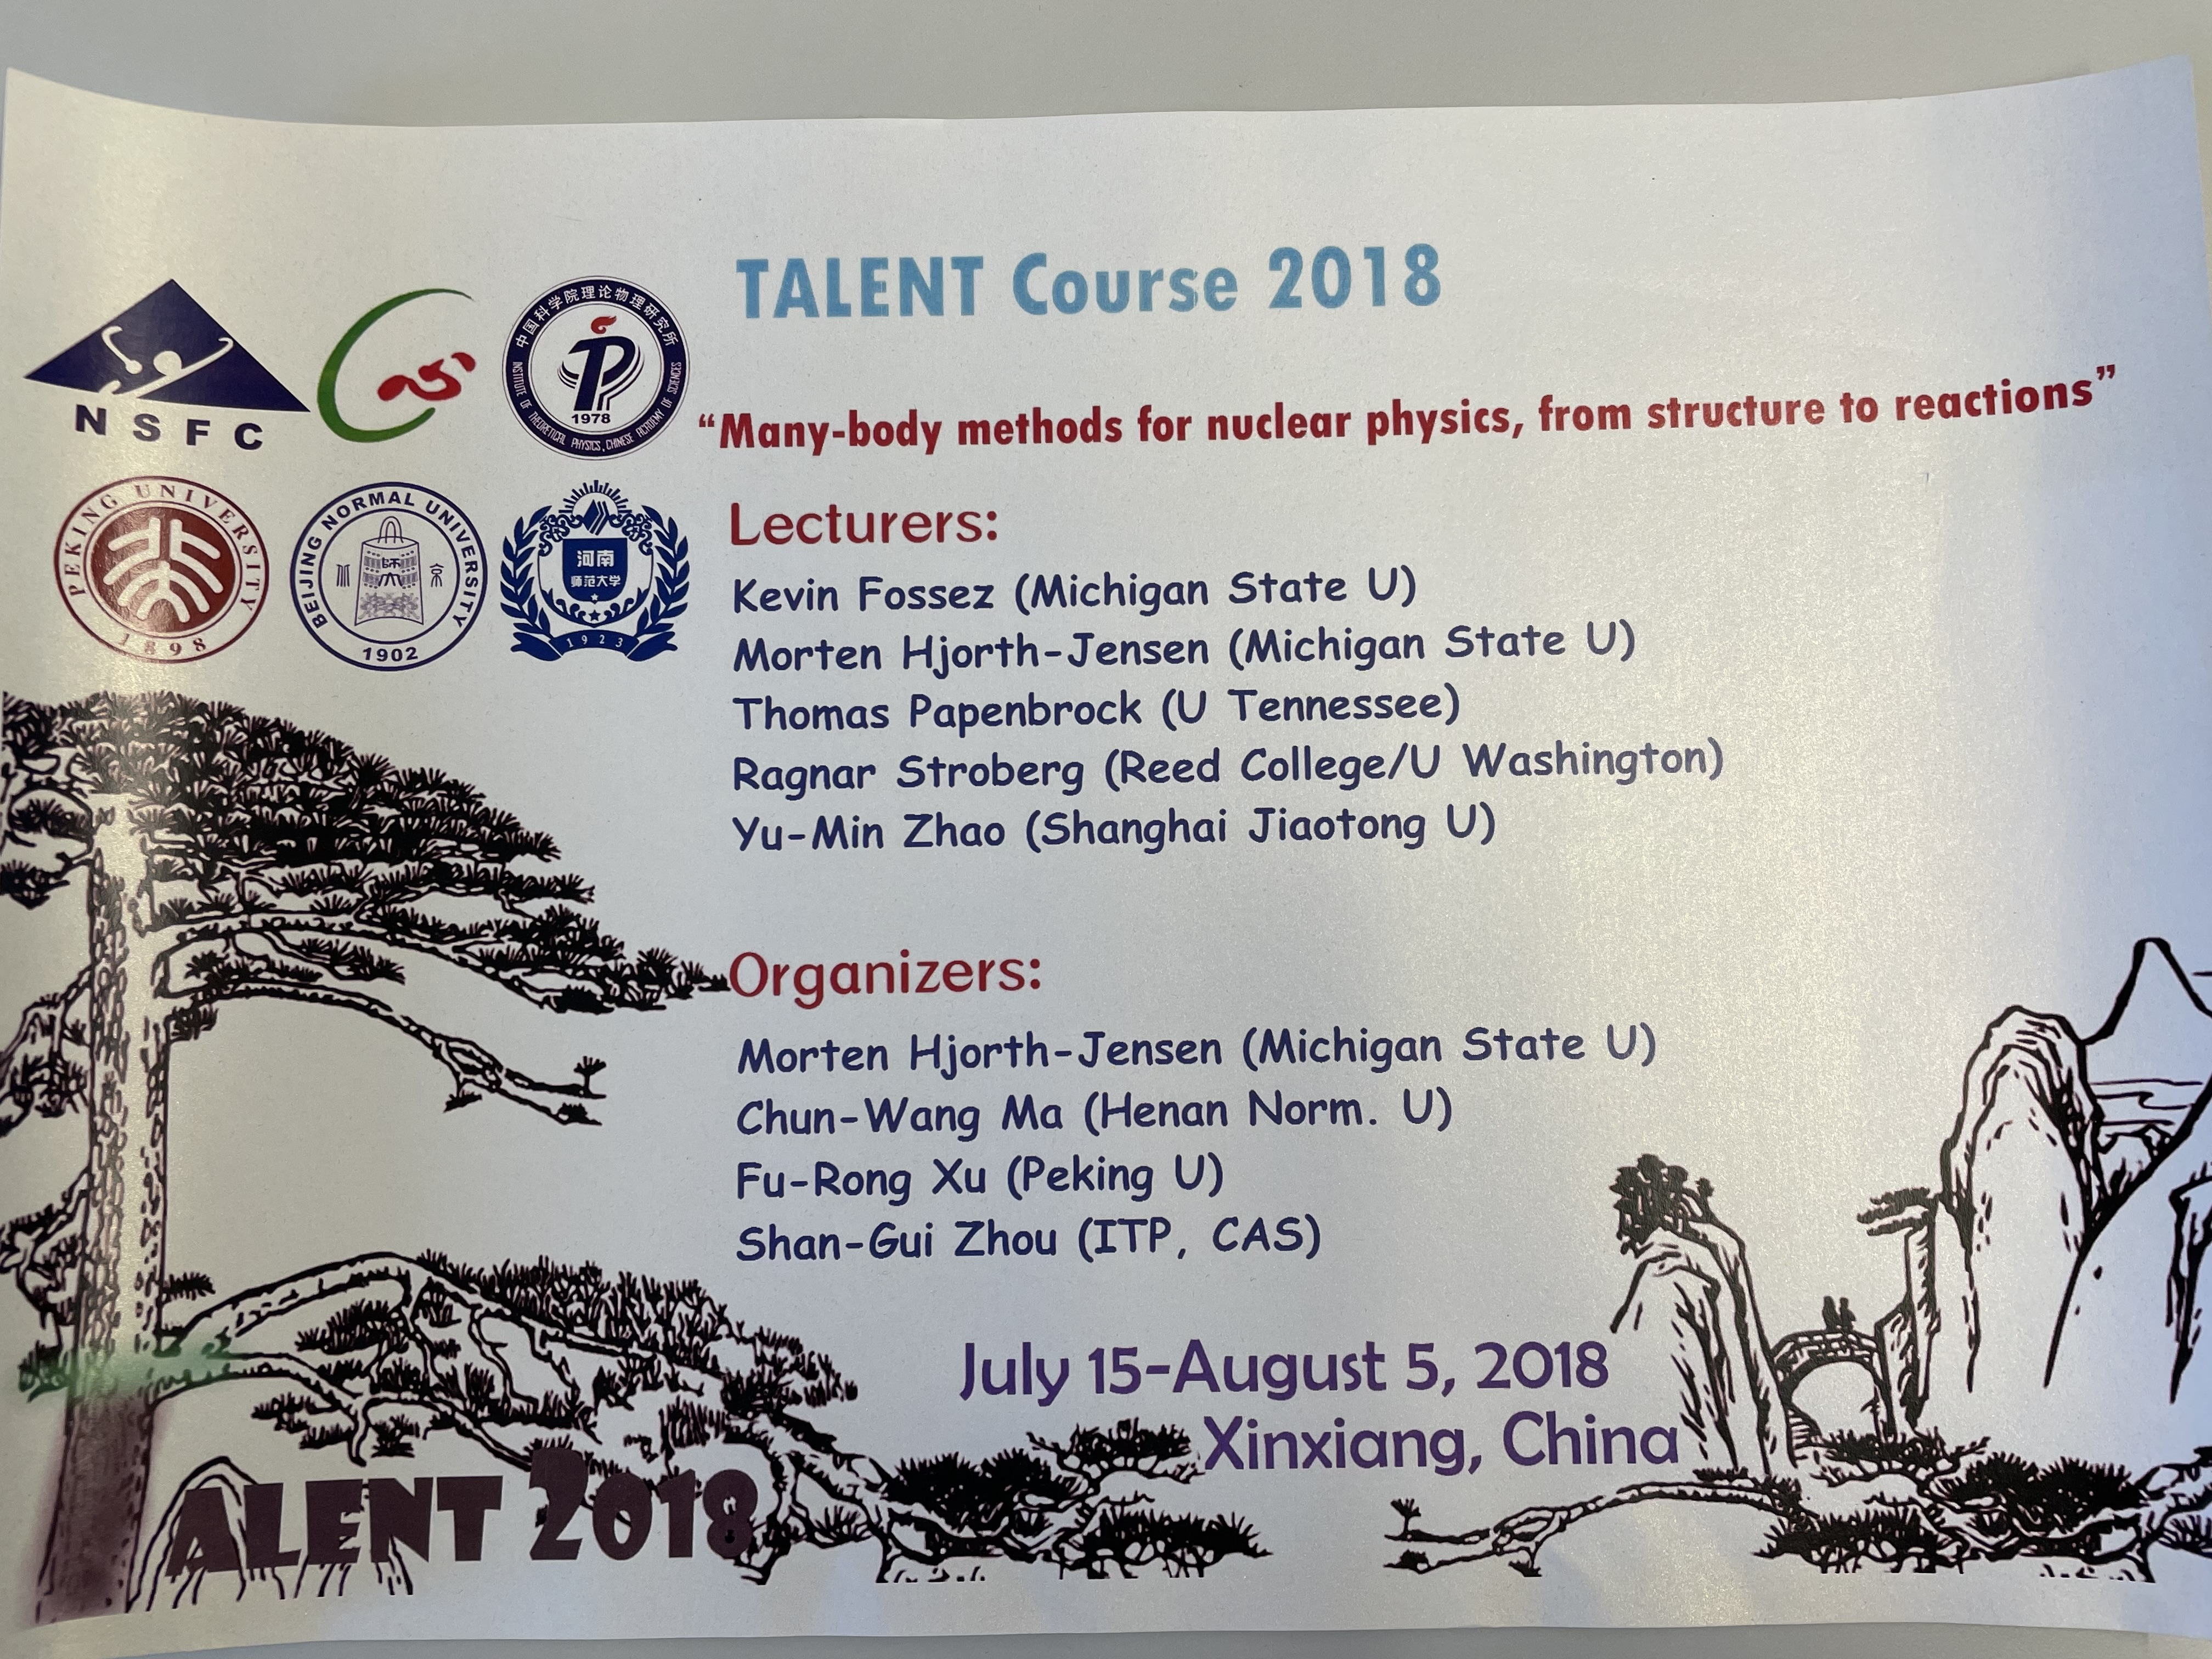
\includegraphics[width=1.0\linewidth]{Photos/talent2018.jpeg}}

\vspace{6mm}
\end{frame}

\begin{frame}[plain,fragile]
\frametitle{Talent courses since 2019, ECT* playing a central role}

\begin{block}{}
\begin{enumerate}
\item \href{{https://www.ectstar.eu/talents/talent-2019/}}{Nuclear TALENT course From Quarks and Gluons to Nuclear Forces and Structure, ECT*, 15 July 2019 — 02 August 2019}

\item \href{{https://www.ectstar.eu/talents/talent-school-special-edition-2020/}}{Nuclear TALENT School on Machine learning from 22 June 2020 to 03 July 2020, ECT* (online)}. 

\item Nuclear TALENT School on Machine learning from 19 July 2021 to  30 July 2021, ECT* (online). 
\end{enumerate}

\noindent
\end{block}

Many lectures from DTPs and Talent courses were collected in a Lecture Notes in Physics volume, see \href{{https://link.springer.com/book/10.1007/978-3-319-53336-0}}{\nolinkurl{https://link.springer.com/book/10.1007/978-3-319-53336-0}}
\end{frame}

\begin{frame}[plain,fragile]
\frametitle{Educational strategies}

The ECT* should continue to play a key role in educating the next generation of nuclear scientists.

\begin{enumerate}
\item Through the organization of DTPs and possibly nuclear Talent courses

\item Be at the forefront in introducing new theoretical developments to nuclear physics (now for example quantum computing and AI/Machine learning)

\item Foster and care for PDs and their careers, develop career plans with European universities and national laboratories, for example larger training networks with selected laboratories and universities. 

\item Similarly, in collaboration with European universities (note the European perspective), develop training networks in nuclear theory at the PhD level and possibly also master level. This has to be done in collaboration with universities.

\item Develop regional, national, European and international initiatives that encompass the above
\end{enumerate}

\noindent
\end{frame}

\begin{frame}[plain,fragile]
\frametitle{And new initiatives}

Introducing the Lattice Virtual Academy (LaVA) by Claudio Bonanno et al, see for example \href{{https://indico.fnal.gov/event/57249/contributions/271752/attachments/169437/227392/talk_LaVA_Bonanno.pdf}}{\nolinkurl{https://indico.fnal.gov/event/57249/contributions/271752/attachments/169437/227392/talk_LaVA_Bonanno.pdf}}.

Under development within STRONG-2020 EU-funded project and technical and financial support by FBK/ECT and by INFN.
\end{frame}

\begin{frame}[plain,fragile]
\frametitle{Machine learning. A simple perspective on the interface between ML and Physics}

\vspace{6mm}

% inline figure
\centerline{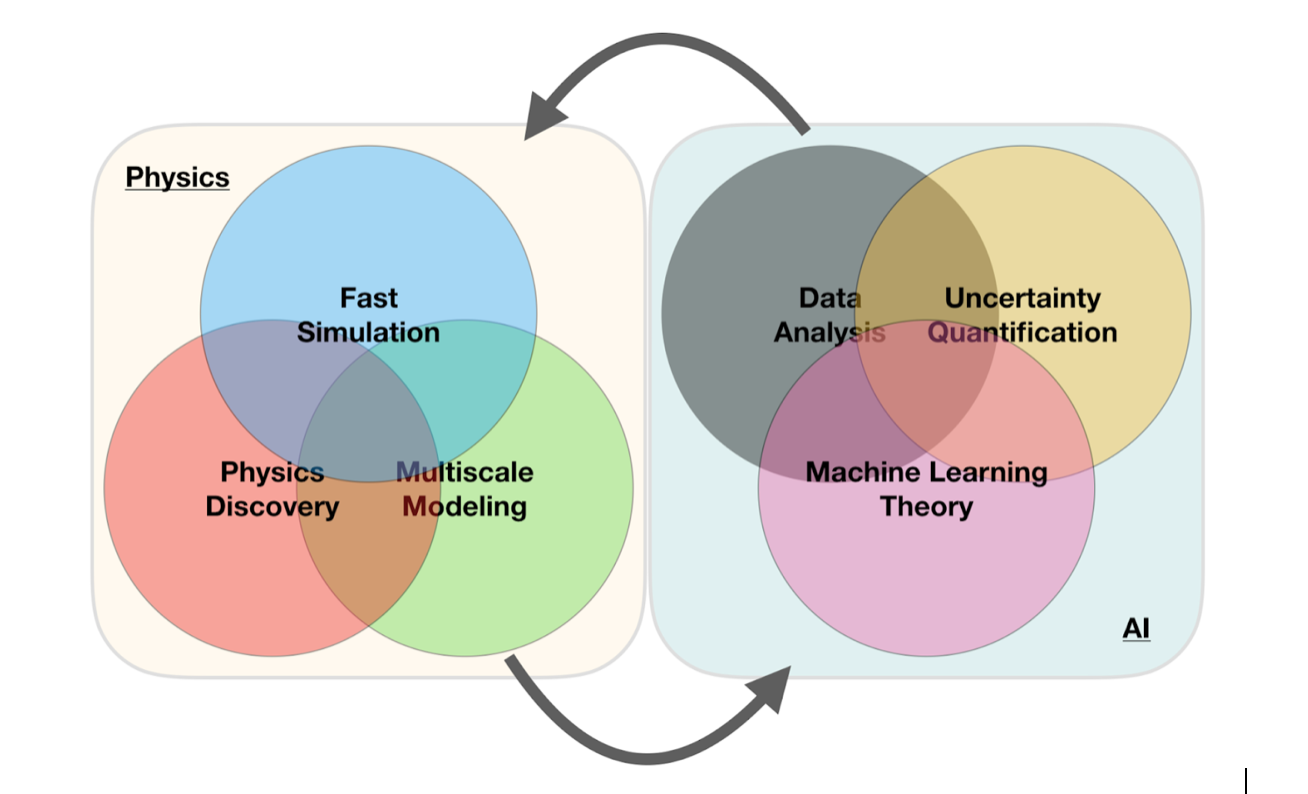
\includegraphics[width=1.0\linewidth]{figures/mlimage.png}}

\vspace{6mm}
\end{frame}

\begin{frame}[plain,fragile]
\frametitle{ML in Nuclear  Physics}

\vspace{6mm}

% inline figure
\centerline{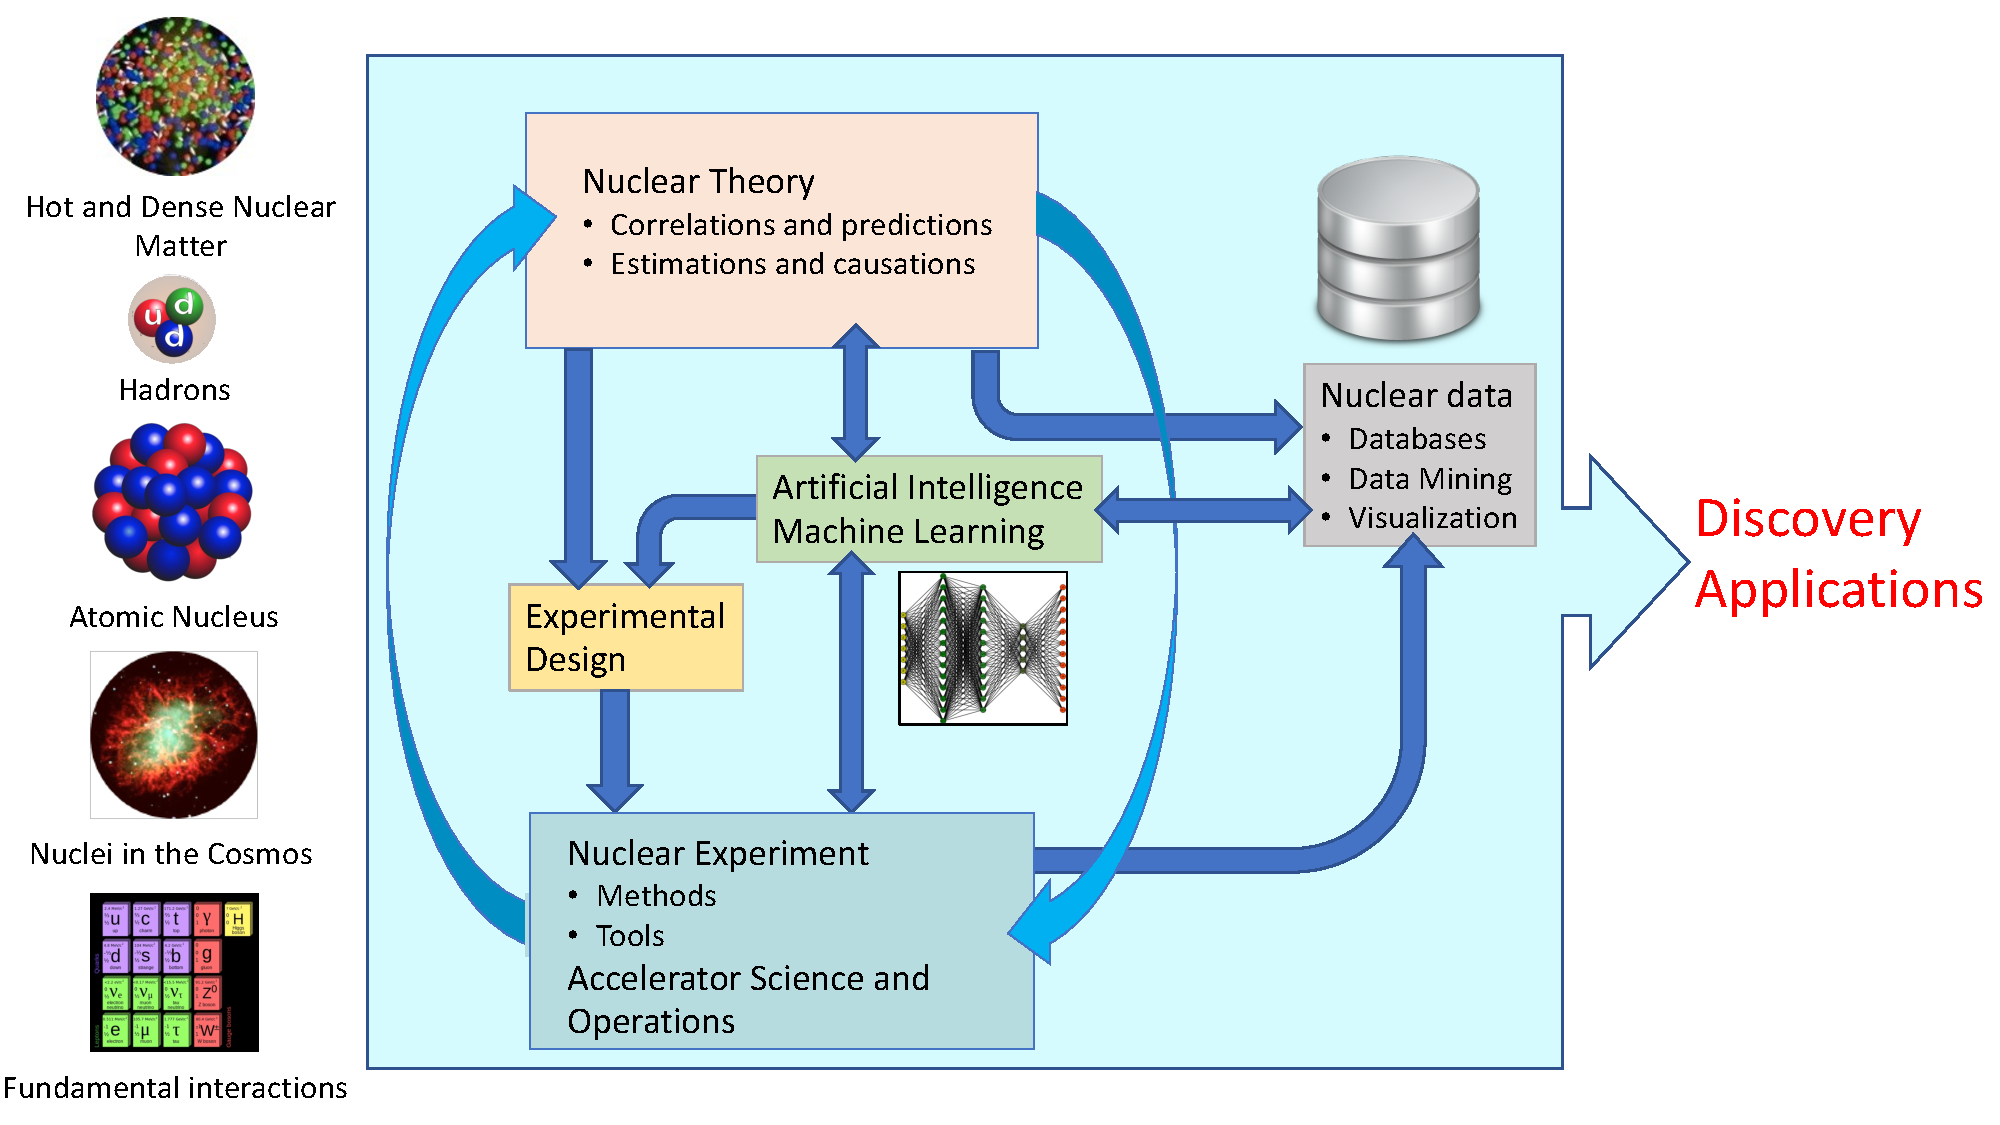
\includegraphics[width=1.0\linewidth]{figures/ML-NP.pdf}}

\vspace{6mm}
\end{frame}

\begin{frame}[plain,fragile]
\frametitle{AI/ML and some statements you may have heard (and what do they mean?)}

\begin{enumerate}
\item Fei-Fei Li on ImageNet: \textbf{map out the entire world of objects} (\href{{https://cacm.acm.org/news/219702-the-data-that-transformed-ai-research-and-possibly-the-world/fulltext}}{The data that transformed AI research})

\item Russell and Norvig in their popular textbook: \textbf{relevant to any intellectual task; it is truly a universal field} (\href{{http://aima.cs.berkeley.edu/}}{Artificial Intelligence, A modern approach})

\item Woody Bledsoe puts it more bluntly: \textbf{in the long run, AI is the only science} (quoted in Pamilla McCorduck, \href{{https://www.pamelamccorduck.com/machines-who-think}}{Machines who think})
\end{enumerate}

\noindent
If you wish to have a critical read on AI/ML from a societal point of view, see \href{{https://www.katecrawford.net/}}{Kate Crawford's recent text Atlas of AI}

\textbf{Here: with AI/ML we intend a collection of machine learning methods with an emphasis on statistical learning and data analysis}
\end{frame}

\begin{frame}[plain,fragile]
\frametitle{Scientific Machine Learning}

An important and emerging field is what has been dubbed as scientific ML, see the article by Deiana et al \href{{https://arxiv.org/abs/2110.13041}}{Applications and Techniques for Fast Machine Learning in Science, arXiv:2110.13041}

\begin{block}{}
The authors discuss applications and techniques for fast machine
learning (ML) in science -- the concept of integrating power ML
methods into the real-time experimental data processing loop to
accelerate scientific discovery. The report covers three main areas

\begin{enumerate}
\item applications for fast ML across a number of scientific domains;

\item techniques for training and implementing performant and resource-efficient ML algorithms;

\item and computing architectures, platforms, and technologies for deploying these algorithms.
\end{enumerate}

\noindent
\end{block}
\end{frame}

\begin{frame}[plain,fragile]
\frametitle{Types of machine learning}

\begin{block}{}
The approaches to machine learning are many, but are often split into two main categories. 
In \emph{supervised learning} we know the answer to a problem,
and let the computer deduce the logic behind it. On the other hand, \emph{unsupervised learning}
is a method for finding patterns and relationship in data sets without any prior knowledge of the system.
Some authours also operate with a third category, namely \emph{reinforcement learning}. This is a paradigm 
of learning inspired by behavioural psychology, where learning is achieved by trial-and-error, 
solely from rewards and punishment.
\end{block}
\end{frame}

\begin{frame}[plain,fragile]
\frametitle{Main categories}

\begin{block}{}
Another way to categorize machine learning tasks is to consider the desired output of a system.
Some of the most common tasks are:

\begin{itemize}
  \item Classification: Outputs are divided into two or more classes. The goal is to   produce a model that assigns inputs into one of these classes. An example is to identify  digits based on pictures of hand-written ones. Classification is typically supervised learning.

  \item Regression: Finding a functional relationship between an input data set and a reference data set.   The goal is to construct a function that maps input data to continuous output values.

  \item Clustering: Data are divided into groups with certain common traits, without knowing the different groups beforehand.  It is thus a form of unsupervised learning.
\end{itemize}

\noindent
\end{block}
\end{frame}

\begin{frame}[plain,fragile]
\frametitle{Machine learning and nuclear theory (my bias): Why?}

\begin{enumerate}
\item ML tools can help us to speed up the scientific process cycle and hence facilitate discoveries

\item Enabling fast emulation for big simulations

\item Revealing the information content of measured observables w.r.t. theory

\item Identifying crucial experimental data for better constraining theory

\item Providing meaningful input to applications and planned measurements

\item ML tools can help us to reveal the structure of our models

\item Parameter estimation with heterogeneous/multi-scale datasets

\item Model reduction

\item ML tools can help us to provide predictive capability

\item Theoretical results often involve ultraviolet  and infrared extrapolations due to Hilbert-space truncations 

\item Uncertainty quantification essential

\item Theoretical models are often applied to entirely new nuclear systems and conditions that are not accessible to experiment
\end{enumerate}

\noindent
\end{frame}

\begin{frame}[plain,fragile]
\frametitle{The plethora  of machine learning algorithms/methods}

\begin{enumerate}
\item Deep learning: Neural Networks (NN), Convolutional NN, Recurrent NN, Boltzmann machines, autoencoders and variational autoencoders  and generative adversarial networks 

\item Bayesian statistics and Bayesian Machine Learning, Bayesian experimental design, Bayesian Regression models, Bayesian neural networks, Gaussian processes and much more

\item Dimensionality reduction (Principal component analysis), Clustering Methods and more

\item Ensemble Methods, Random forests, bagging and voting methods, gradient boosting approaches 

\item Linear and logistic regression, Kernel methods, support vector machines and more

\item Reinforcement Learning 

\item Generative models and more
\end{enumerate}

\noindent
\end{frame}

\begin{frame}[plain,fragile]
\frametitle{Examples of Machine Learning methods and applications in nuclear physics}

\begin{block}{}
\begin{itemize}
\item \textbf{Machine  learning  for  data  mining:} Oftentimes,  it  is necessary to be able to accurately calculate observables that have not been measured, to supplement the existing databases.

\item \textbf{Nuclear  density  functional   theory:} Energy density functional calibration   involving Bayesian optimization  and ML.

\item \textbf{Nuclear properties with ML:} Improving predictive power of nuclear models by emulating model residuals.

\item \textbf{Effective field theory and A-body systems:} Truncation errors and low-energy coupling constant calibration, nucleon-nucleon scattering calculations, variational calculations with ANN for light nuclei, NN extrapolation of nuclear structure observables

\item \textbf{Nuclear  shell  model  UQ:} ML methods  have  been  used  to  provide  UQ  of  configuration  interaction  calculations.
\end{itemize}

\noindent
\end{block}
\end{frame}

\begin{frame}[plain,fragile]
\frametitle{Examples of Machine Learning methods and applications in nuclear physics, continues}

\begin{block}{}
\begin{itemize}
\item \textbf{Low-energy nuclear reactions UQ:} Bayesian optimization studies of the nucleon-nucleus optical potential, R-matrix analyses,  and  statistical spatial networks to study patterns in nuclear reaction networks.

\item \textbf{Neutron star properties and nuclear matter equation of state:} constraining the equation of state by properties on neutron stars and selected properties of finite nuclei

\item \textbf{Experimental design:} Bayesian ML provides a framework  to  maximize  the  success  of  on  experiment  based on  the  best  information  available  on existing  data, experimental conditions, and theoretical models.
\end{itemize}

\noindent
\end{block}
\end{frame}

\begin{frame}[plain,fragile]
\frametitle{More examples}

The large amount of degrees of freedom pertain to both theory and experiment in nuclear physics. With increasingly complicated experiments that produce large amounts data, automated classification of events becomes increasingly important. Here, deep learning methods offer a plethora of interesting research avenues. 

\begin{block}{}
\begin{itemize}
\item Reconstruction of particle trajectories or classification of events are typical examples where ML methods are being used. However, since these data can often be extremely noisy, the precision necessary for discovery in physics requires algorithmic improvements. Research along such directions, interfacing nuclear physics with AI/ML is expected to play a significant role in physics discoveries related to new facilities.  The treatment of corrupted data in imaging and image processing is also a relevant topic. 

\item Design of detectors represents an important area of applications for ML/AI methods in nuclear physics.
\end{itemize}

\noindent
\end{block}
\end{frame}

\begin{frame}[plain,fragile]
\frametitle{And more}

\begin{block}{}
\begin{itemize}
\item An important application of AI/ML methods is to improve the estimation of bias or uncertainty due to the introduction of or lack of physical constraints in various theoretical models.

\item In theory, we expect to use AI/ML algorithms and methods to improve our knowledge about  correlations of physical model parameters in data for quantum many-body systems. Deep learning methods show great promise in circumventing the exploding dimensionalities encountered in quantum mechanical many-body studies. 

\item Merging a frequentist approach (the standard path in ML theory) with a Bayesian approach, has the potential to infer better probabilitity distributions and error estimates. As an example, methods for fast Monte-Carlo- based Bayesian computation of nuclear density functionals show great promise in providing a better understanding 

\item Machine Learning and Quantum Computing is a very interesting avenue to explore. 
\end{itemize}

\noindent
\end{block}
\end{frame}

\begin{frame}[plain,fragile]
\frametitle{Selected references}

\begin{block}{}
\begin{itemize}
\item \href{{https://arxiv.org/abs/1803.08823}}{Mehta et al.} and \href{{https://www.sciencedirect.com/science/article/pii/S0370157319300766?via%3Dihub}}{Physics Reports (2019)}.

\item \href{{https://link.aps.org/doi/10.1103/RevModPhys.91.045002}}{Machine Learning and the Physical Sciences by Carleo et al}

\item \href{{https://journals.aps.org/rmp/abstract/10.1103/RevModPhys.94.031003}}{Artificial Intelligence and Machine Learning in Nuclear Physics, Amber Boehnlein et al., Reviews Modern of Physics 94, 031003 (2022)} 

\item \href{{https://journals.aps.org/prresearch/pdf/10.1103/PhysRevResearch.5.033062}}{Dilute neutron star matter from neural-network quantum states by Fore et al, Physical Review Research 5, 033062 (2023)}

\item \href{{https://doi.org/10.48550/arXiv.2305.08831}}{Neural-network quantum states for ultra-cold Fermi gases, Jane Kim et al, Nature Physics Communcication, submitted}

\item \href{{https://doi.org/10.48550/arXiv.2305.07240}}{Message-Passing Neural Quantum States for the Homogeneous Electron Gas, Gabriel Pescia, Jane Kim et al.~arXiv.2305.07240,}

\item \href{{https://doi.org/10.3389/fphy.2023.1061580}}{Efficient solutions of fermionic systems using artificial neural networks, Nordhagen et al, Frontiers in Physics 11, 2023}

\item \href{{https://link.springer.com/article/10.1140/epja/s10050-020-00290-x}}{Report from the A.I. For Nuclear Physics  Workshop by Bedaque et al., Eur J. Phys. A 57, (2021)}

\item \href{{https://pdg.lbl.gov/2021/reviews/rpp2021-rev-machine-learning.pdf}}{Particle Data Group summary on ML methods}
\end{itemize}

\noindent
\end{block}
\end{frame}

\begin{frame}[plain,fragile]
\frametitle{What are the basic ingredients?}

\begin{block}{}
Almost every problem in ML and data science starts with the same ingredients:
\begin{itemize}
\item The dataset $\mathbf{x}$ (could be some observable quantity of the system we are studying)

\item A model which is a function of a set of parameters $\mathbf{\alpha}$ that relates to the dataset, say a likelihood  function $p(\mathbf{x}\vert \mathbf{\alpha})$ or just a simple model $f(\mathbf{\alpha})$

\item A so-called \textbf{loss/cost/risk} function $\mathcal{C} (\mathbf{x}, f(\mathbf{\alpha}))$ which allows us to decide how well our model represents the dataset. 
\end{itemize}

\noindent
We seek to minimize the function $\mathcal{C} (\mathbf{x}, f(\mathbf{\alpha}))$ by finding the parameter values which minimize $\mathcal{C}$. This leads to  various minimization algorithms. It may surprise many, but at the heart of all machine learning algortihms there is an optimization problem. 
\end{block}
\end{frame}

\begin{frame}[plain,fragile]
\frametitle{Argon-46 by Solli et al., NIMA 1010, 165461 (2021)}

\begin{block}{}
Representations of two events from the
Argon-46 experiment. Each row is one event in two projections,
where the color intensity of each point indicates higher charge values
recorded by the detector. The bottom row illustrates a carbon event with
a large fraction of noise, while the top row shows a proton event
almost free of noise. 
\end{block}

\vspace{6mm}

% inline figure
\centerline{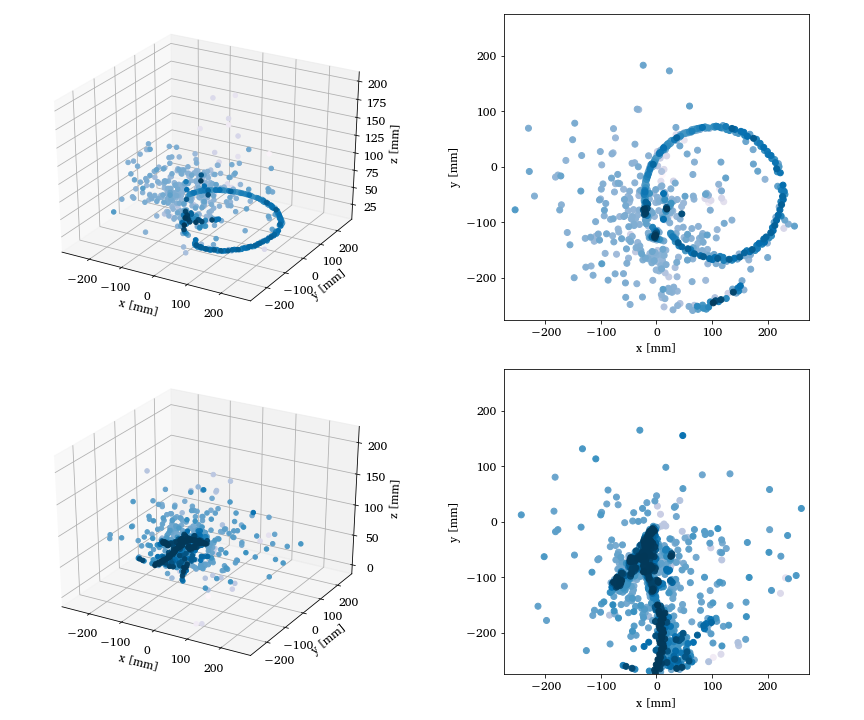
\includegraphics[width=0.6\linewidth]{figures/examples_raw.png}}

\vspace{6mm}
\end{frame}

\begin{frame}[plain,fragile]
\frametitle{Many-body physics, Quantum Monte Carlo and deep learning}

\begin{block}{}
Given a hamiltonian $H$ and a trial wave function $\Psi_T$, the variational principle states that the expectation value of $\langle H \rangle$, defined through 
\[
   \langle E \rangle =
   \frac{\int d\bm{R}\Psi^{\ast}_T(\bm{R})H(\bm{R})\Psi_T(\bm{R})}
        {\int d\bm{R}\Psi^{\ast}_T(\bm{R})\Psi_T(\bm{R})},
\]
is an upper bound to the ground state energy $E_0$ of the hamiltonian $H$, that is 
\[
    E_0 \le \langle E \rangle.
\]
In general, the integrals involved in the calculation of various  expectation values  are multi-dimensional ones. Traditional integration methods such as the Gauss-Legendre will not be adequate for say the  computation of the energy of a many-body system.  \textbf{Basic philosophy: Let a neural network find the optimal wave function}
\end{block}
\end{frame}

\begin{frame}[plain,fragile]
\frametitle{Monte Carlo methods and Neural Networks}

\href{{https://www.sciencedirect.com/science/article/pii/S0370269320305463?via%3Dihub}}{Machine Learning and the Deuteron by Kebble and Rios} and
\href{{https://journals.aps.org/prl/abstract/10.1103/PhysRevLett.127.022502}}{Variational Monte Carlo calculations of $A\le 4$ nuclei with an artificial neural-network correlator ansatz by Adams et al.}

\textbf{Adams et al}:

\begin{align}
H_{LO} &=-\sum_i \frac{{\vec{\nabla}_i^2}}{2m_N}
+\sum_{i<j} {\left(C_1  + C_2\, \vec{\sigma_i}\cdot\vec{\sigma_j}\right)
e^{-r_{ij}^2\Lambda^2 / 4 }}
\nonumber\\
&+D_0 \sum_{i<j<k} \sum_{\text{cyc}}
{e^{-\left(r_{ik}^2+r_{ij}^2\right)\Lambda^2/4}}\,,
\end{align}

where $m_N$ is the mass of the nucleon, $\vec{\sigma_i}$ is the Pauli
matrix acting on nucleon $i$, and $\sum_{\text{cyc}}$ stands for the
cyclic permutation of $i$, $j$, and $k$. The low-energy constants
$C_1$ and $C_2$ are fit to the deuteron binding energy and to the
neutron-neutron scattering length
\end{frame}

\begin{frame}[plain,fragile]
\frametitle{Deep learning neural networks, \href{{https://journals.aps.org/prl/abstract/10.1103/PhysRevLett.127.022502}}{Variational Monte Carlo calculations of $A\le 4$ nuclei with an artificial neural-network correlator ansatz by Adams et al.}}

An appealing feature of the neural network ansatz is that it is more general than the more conventional product of two-
and three-body spin-independent Jastrow functions
\begin{align}
|\Psi_V^J \rangle = \prod_{i<j<k} \Big( 1-\sum_{\text{cyc}} u(r_{ij}) u(r_{jk})\Big) \prod_{i<j} f(r_{ij}) | \Phi\rangle\,,
\end{align}
which is commonly used for nuclear Hamiltonians that do not contain tensor and spin-orbit terms.
The above function is replaced by a four-layer Neural Network.
\end{frame}

\begin{frame}[plain,fragile]
\frametitle{Explicit results}

\vspace{6mm}

% inline figure
\centerline{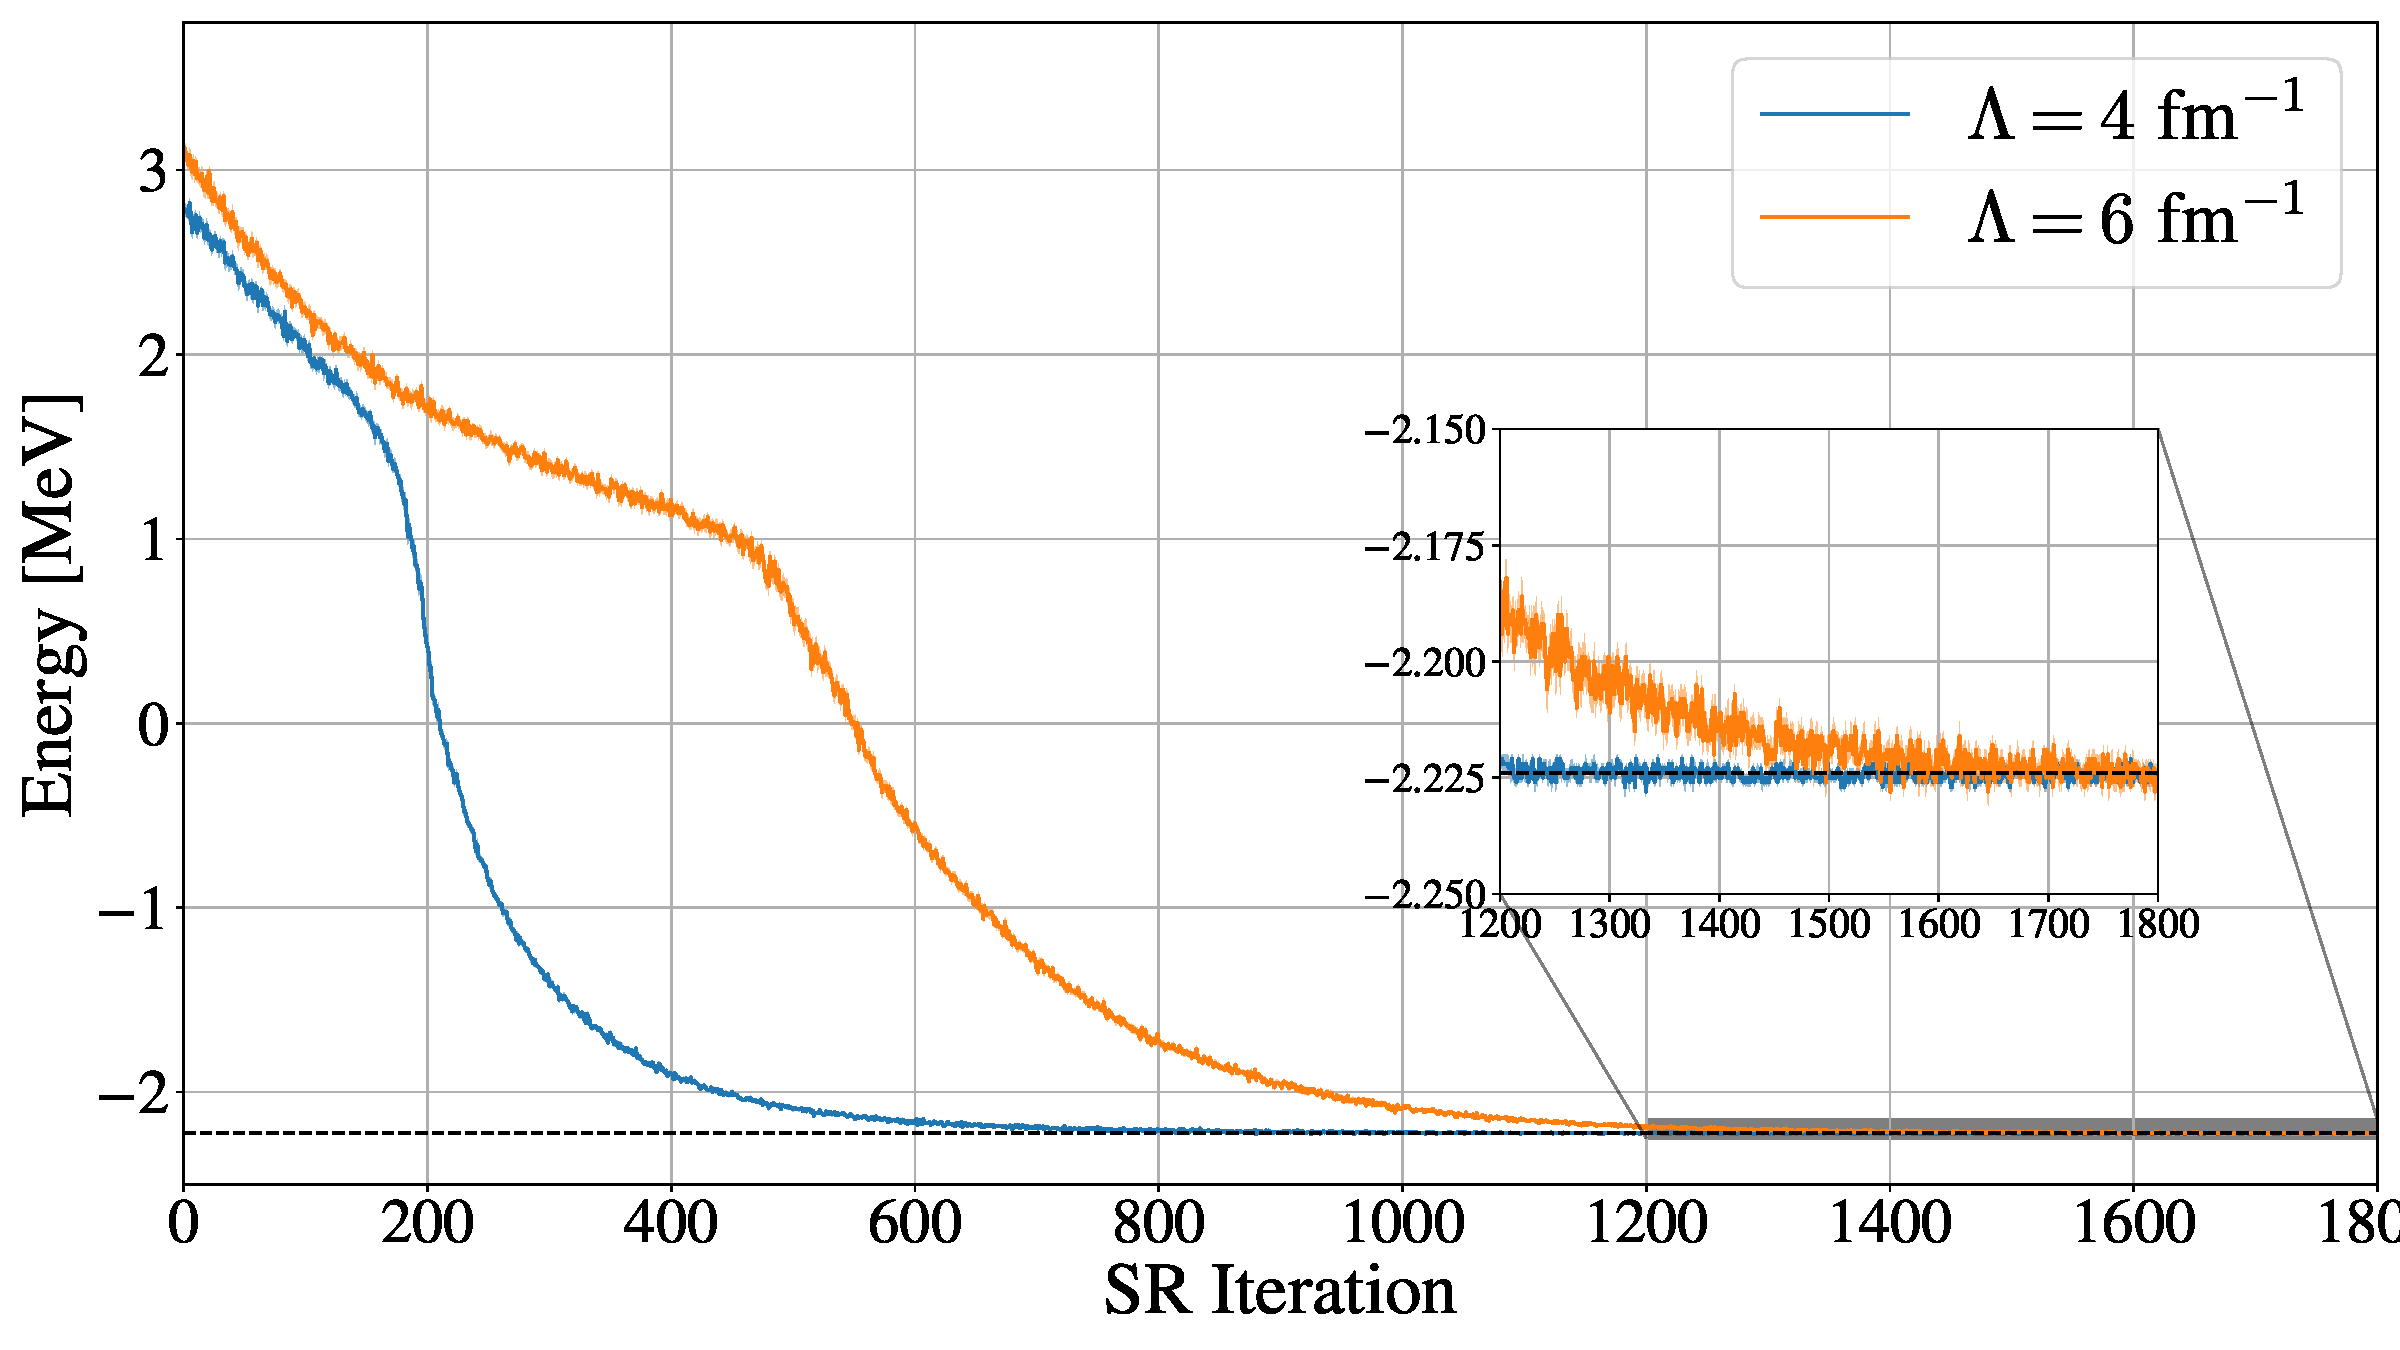
\includegraphics[width=0.9\linewidth]{figures/energyconvergence.pdf}}

\vspace{6mm}
\end{frame}

\begin{frame}[plain,fragile]
\frametitle{\href{{https://journals.aps.org/prresearch/pdf/10.1103/PhysRevResearch.5.033062}}{Dilute neutron star matter from neural-network quantum states by Fore et al, Physical Review Research 5, 033062 (2023)} at density $\rho=0.04$ fm$^{-3}$}

\begin{block}{}

\vspace{6mm}

% inline figure
\centerline{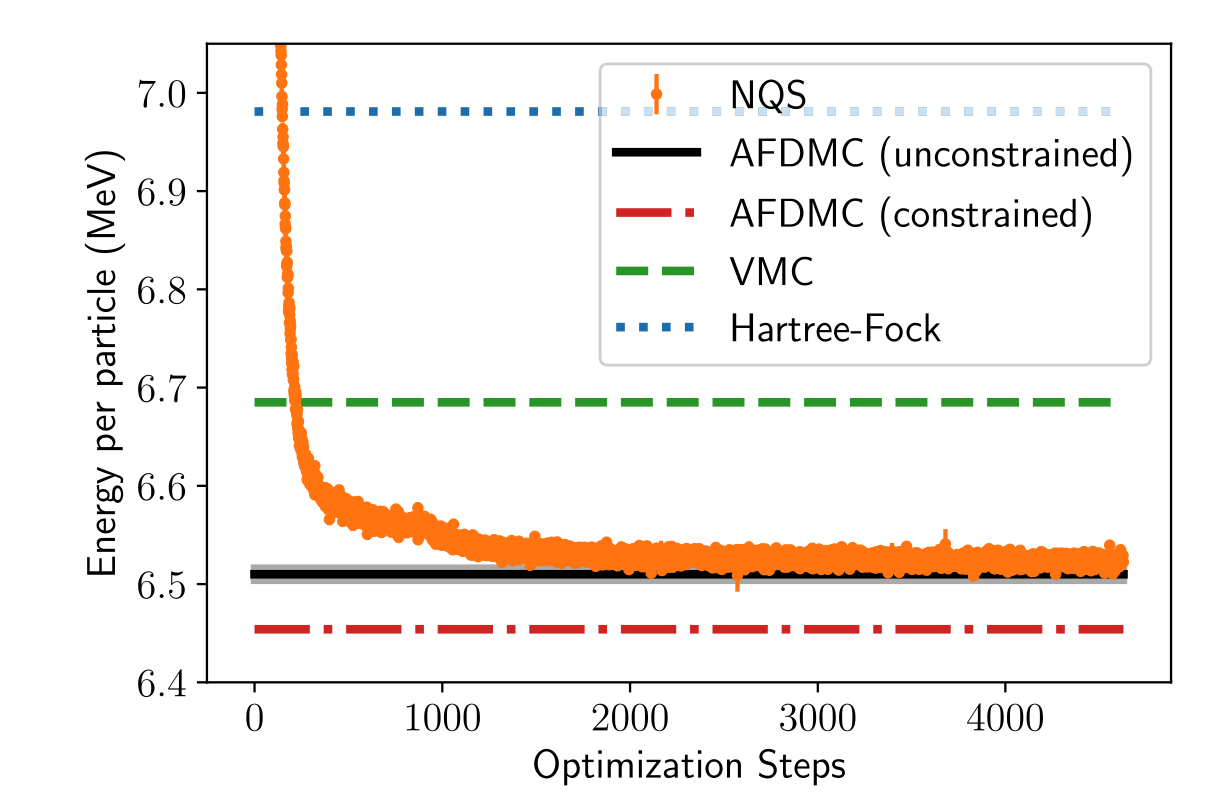
\includegraphics[width=0.9\linewidth]{figures/nmatter.png}}

\vspace{6mm}

\end{block}
\end{frame}

\begin{frame}[plain,fragile]
\frametitle{The electron gas in three dimensions with $N=14$ electrons (Wigner-Seitz radius $r_s=2$ a.u.), \href{{https://doi.org/10.48550/arXiv.2305.07240}}{Gabriel Pescia, Jane Kim et al.~arXiv.2305.07240,}}

\begin{block}{}

\vspace{6mm}

% inline figure
\centerline{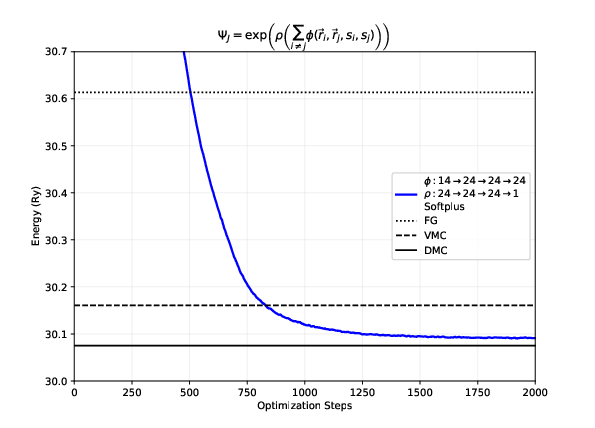
\includegraphics[width=0.9\linewidth]{figures/elgasnew.png}}

\vspace{6mm}

\end{block}
\end{frame}

\begin{frame}[plain,fragile]
\frametitle{\href{{https://doi.org/10.3389/fphy.2023.1061580}}{Efficient solutions of fermionic systems using artificial neural networks, Nordhagen et al, Frontiers in Physics 11, 2023}}

The Hamiltonian of the quantum dot is given by
\[ \hat{H} = \hat{H}_0 + \hat{V}, 
\]
where $\hat{H}_0$ is the many-body HO Hamiltonian, and $\hat{V}$ is the
inter-electron Coulomb interactions. In dimensionless units,
\[ \hat{V}= \sum_{i < j}^N \frac{1}{r_{ij}},
\]
with $r_{ij}=\sqrt{\mathbf{r}_i^2 - \mathbf{r}_j^2}$.

This leads to the  separable Hamiltonian, with the relative motion part given by ($r_{ij}=r$)
\[ 
\hat{H}_r=-\nabla^2_r + \frac{1}{4}\omega^2r^2+ \frac{1}{r},
\]
plus a standard Harmonic Oscillator problem  for the center-of-mass motion.
This system has analytical solutions in two and three dimensions (\href{{https://journals.aps.org/pra/abstract/10.1103/PhysRevA.48.3561}}{M. Taut 1993 and 1994}).
\end{frame}

\begin{frame}[plain,fragile]
\frametitle{Quantum dots and Boltzmann machines, onebody densities $N=6$, $\hbar\omega=0.1$ a.u.}

\begin{block}{}

\vspace{6mm}

% inline figure
\centerline{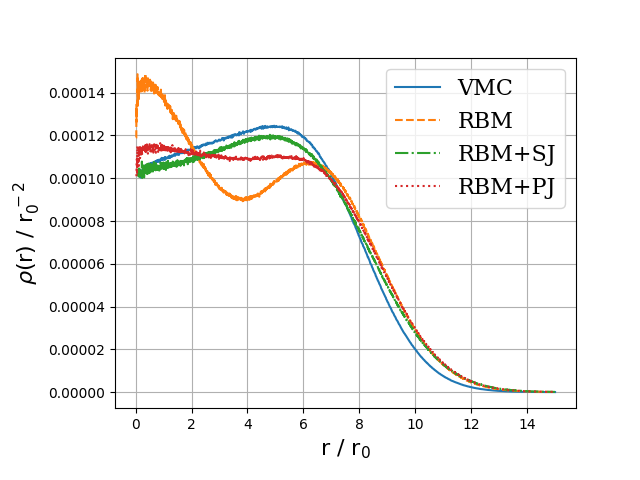
\includegraphics[width=0.9\linewidth]{figures/OB6hw01.png}}

\vspace{6mm}

\end{block}
\end{frame}

\begin{frame}[plain,fragile]
\frametitle{Onebody densities $N=30$, $\hbar\omega=1.0$ a.u.}

\begin{block}{}

\vspace{6mm}

% inline figure
\centerline{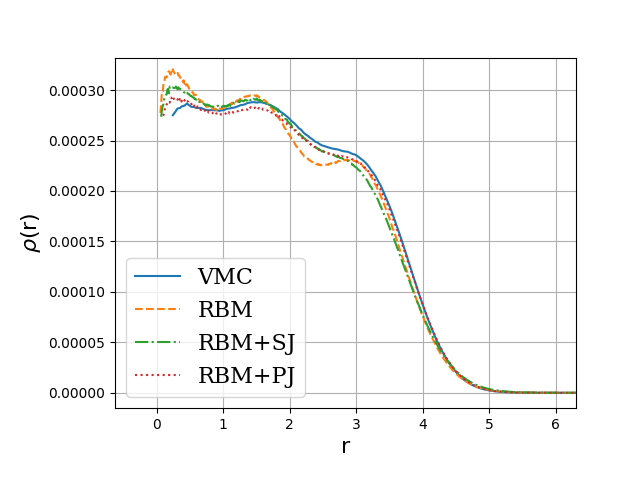
\includegraphics[width=0.9\linewidth]{figures/OB30hw1.png}}

\vspace{6mm}

\end{block}
\end{frame}

\begin{frame}[plain,fragile]
\frametitle{Onebody densities $N=30$, $\hbar\omega=0.1$ a.u.}

\begin{block}{}

\vspace{6mm}

% inline figure
\centerline{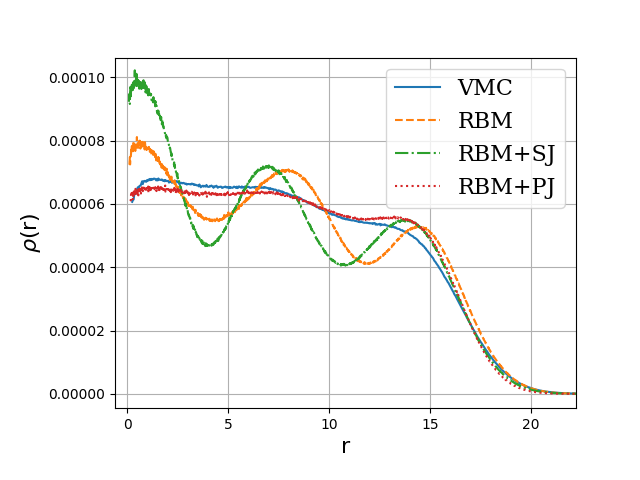
\includegraphics[width=0.9\linewidth]{figures/OB30hw01.png}}

\vspace{6mm}

\end{block}
\end{frame}

\begin{frame}[plain,fragile]
\frametitle{Quantified limits of the nuclear landscape}

\href{{https://journals.aps.org/prc/abstract/10.1103/PhysRevC.101.044307}}{Neufcourt et al., Phys. Rev. C 101, 044307 (2020)}
Predictions made with eleven global mass model and Bayesian model averaging

\vspace{6mm}

% inline figure
\centerline{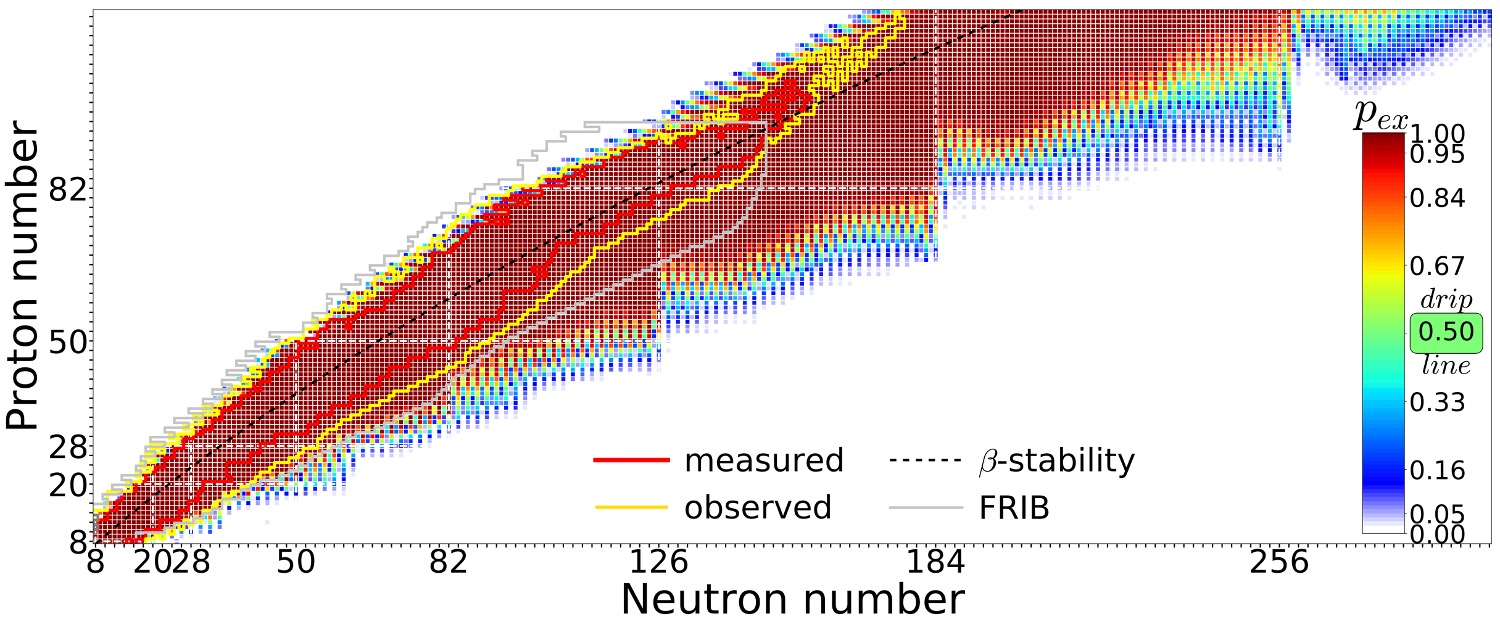
\includegraphics[width=1.0\linewidth]{figures/landscape.jpg}}

\vspace{6mm}
\end{frame}

\begin{frame}[plain,fragile]
\frametitle{Constraining the equation of state for dense nuclear matter}

\href{{https://iopscience.iop.org/article/10.3847/2041-8213/ab822f}}{G. Raaijmakers et al., Constraining the Dense Matter Equation of State with Joint Analysis of NICER and LIGO/Virgo Measurements, AJ Letters, 893, L21 (2020)}

\vspace{6mm}

% inline figure
\centerline{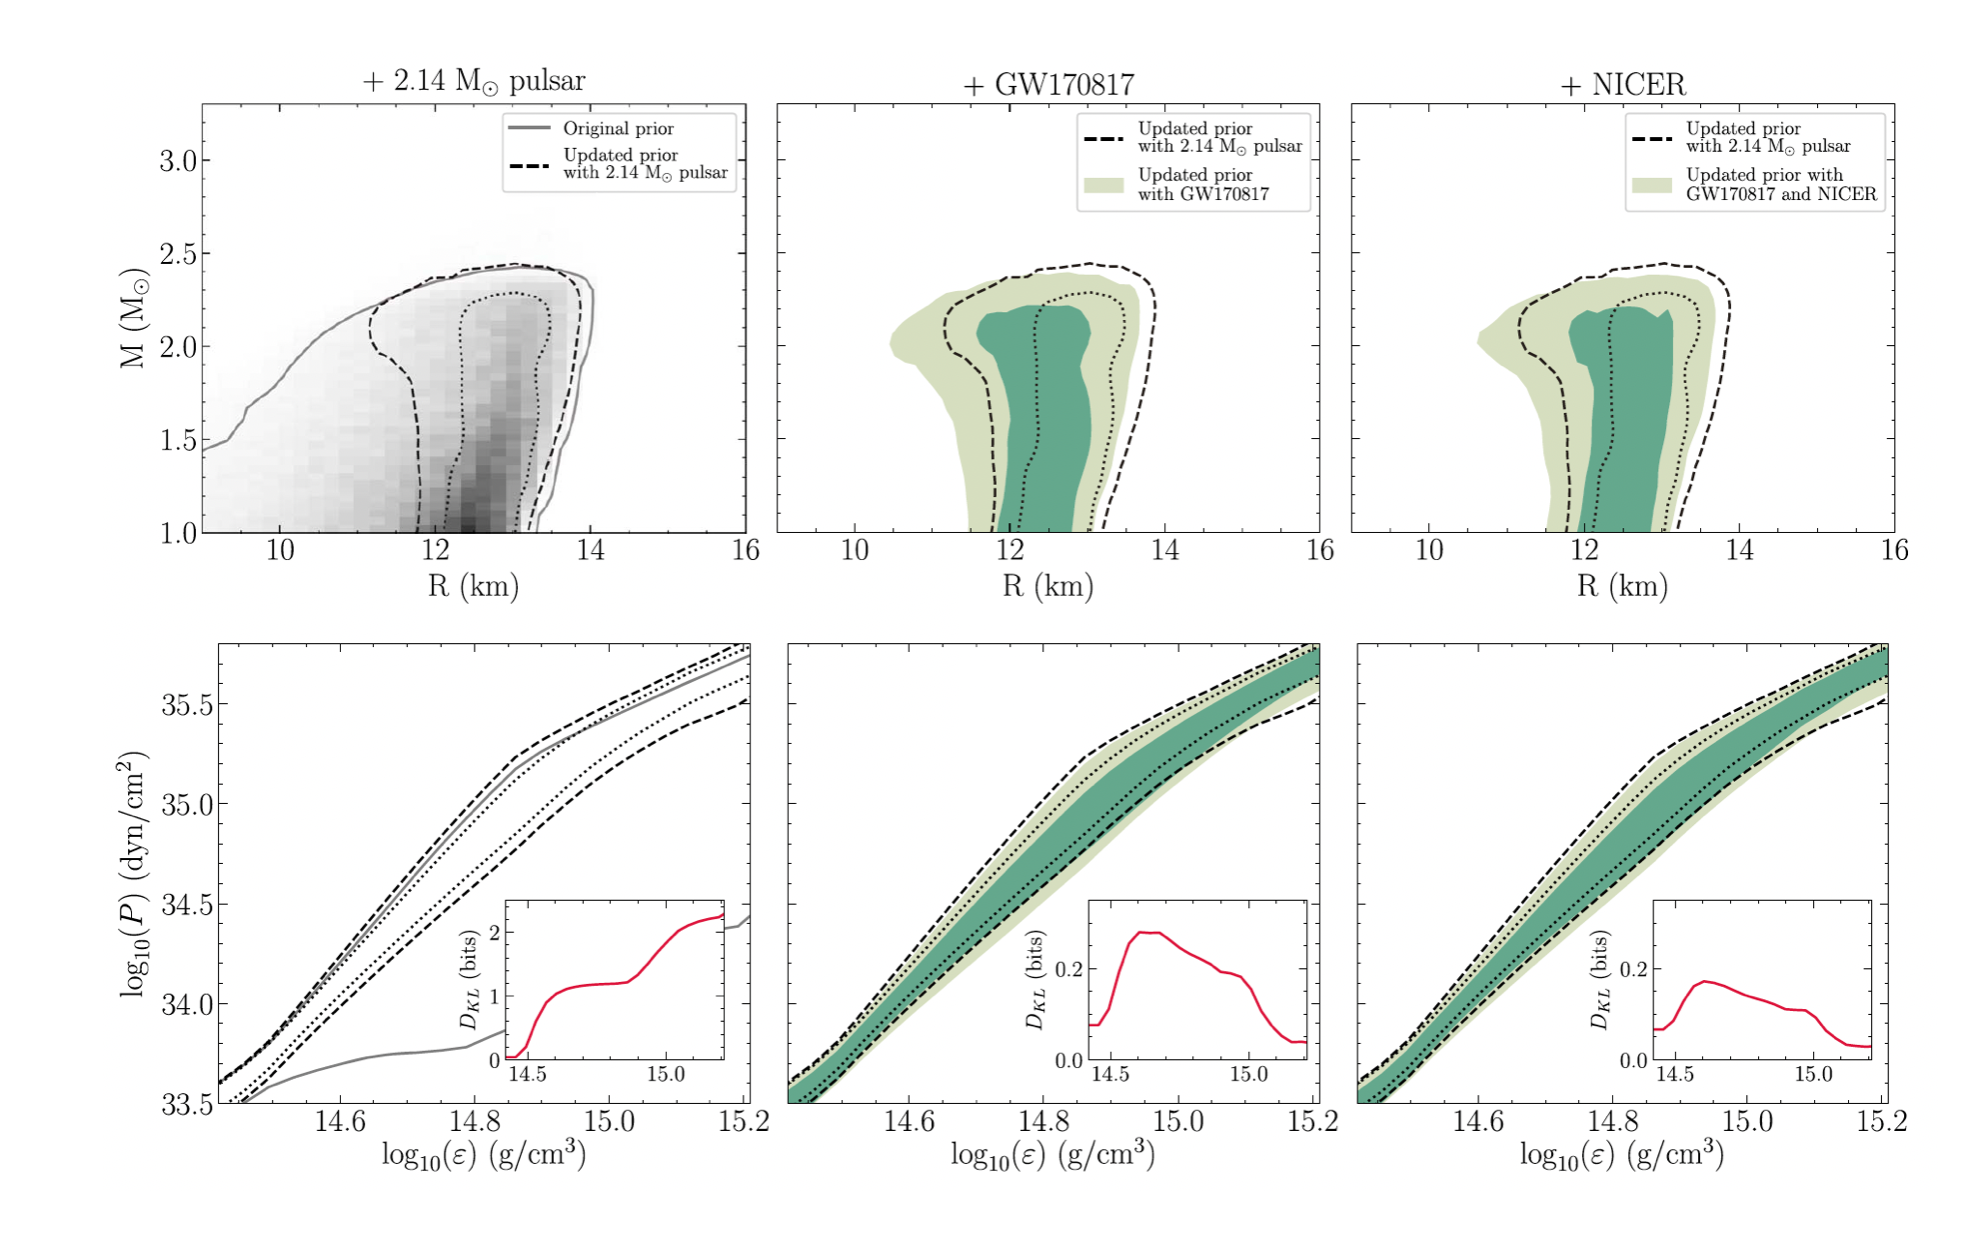
\includegraphics[width=1.0\linewidth]{figures/nstareos.png}}

\vspace{6mm}
\end{frame}

\begin{frame}[plain,fragile]
\frametitle{Experimental design}

Beam time and compute cycles are expensive!

\begin{itemize}
\item Bayesian experimental design provides a framework in which experiments can be designed using the best experimental and theoretical information available 

\item The utility function is designed to encode the goals of the experiment and the constraints inherent in carrying it out. 

\item Once the utility function and the possible designs have been specified, the optimal design is simply the scenario that  maximizes the expected utility function over the domain of possible designs.
\end{itemize}

\noindent
\end{frame}

\begin{frame}[plain,fragile]
\frametitle{Observations and perspectives}

\begin{block}{}
\begin{itemize}
\item Need for AI/Machine Learning in nuclear physics, lots of ongoing activities

\item To solve many complex problems in the field and facilitate discoveries, multidisciplinary efforts efforts are required involving scientists in  nuclear physics, statistics, computational science, and applied math.

\item There is a need for  focused AI/ML learning efforts that will benefit accelerator science and experimental and theoretical programs
\end{itemize}

\noindent
\end{block}
\end{frame}

\begin{frame}[plain,fragile]
\frametitle{How can we use ML in Nuclear Science?}

\begin{block}{}
\begin{itemize}
\item How do we develop insights, competences, knowledge in statistical learning that can advance our field?
\begin{itemize}

  \item For example: Can we use ML to find out which correlations are relevant and thereby diminish the dimensionality problem in standard many-body  theories?

  \item Can we use AI/ML in detector analysis, accelerator design, analysis of experimental data and more?

  \item Can we use AL/ML to carry out reliable extrapolations by using current experimental knowledge and current theoretical models?

  \item Future research may have a strong focus on generative models

\end{itemize}

\noindent
\item The community needs to invest in relevant educational efforts and training of nuclear physicists with knowledge in AI/ML

\item Most likely tons of things we have forgotten
\end{itemize}

\noindent
\end{block}
\end{frame}

\begin{frame}[plain,fragile]
\frametitle{Possible start to raise awareness about ML in our field}

\begin{block}{}
\begin{itemize}
\item Make an ML challenge in nuclear physics a la \href{{https://home.cern/news/news/computing/higgs-boson-machine-learning-challenge}}{Learning to discover: the Higgs boson machine learning challenge}. Alternatively go to kaggle.com at \href{{https://www.kaggle.com/c/higgs-boson}}{\nolinkurl{https://www.kaggle.com/c/higgs-boson}}

\item HEP@CERN and HEP in general have made significant impacts in the field of machine learning and AI. Something to learn from
\end{itemize}

\noindent
\end{block}
\end{frame}

\begin{frame}[plain,fragile]
\frametitle{Villa Tambosi, summer 1995, Tempus Fugit (sadly)}

\vspace{6mm}

% inline figure
\centerline{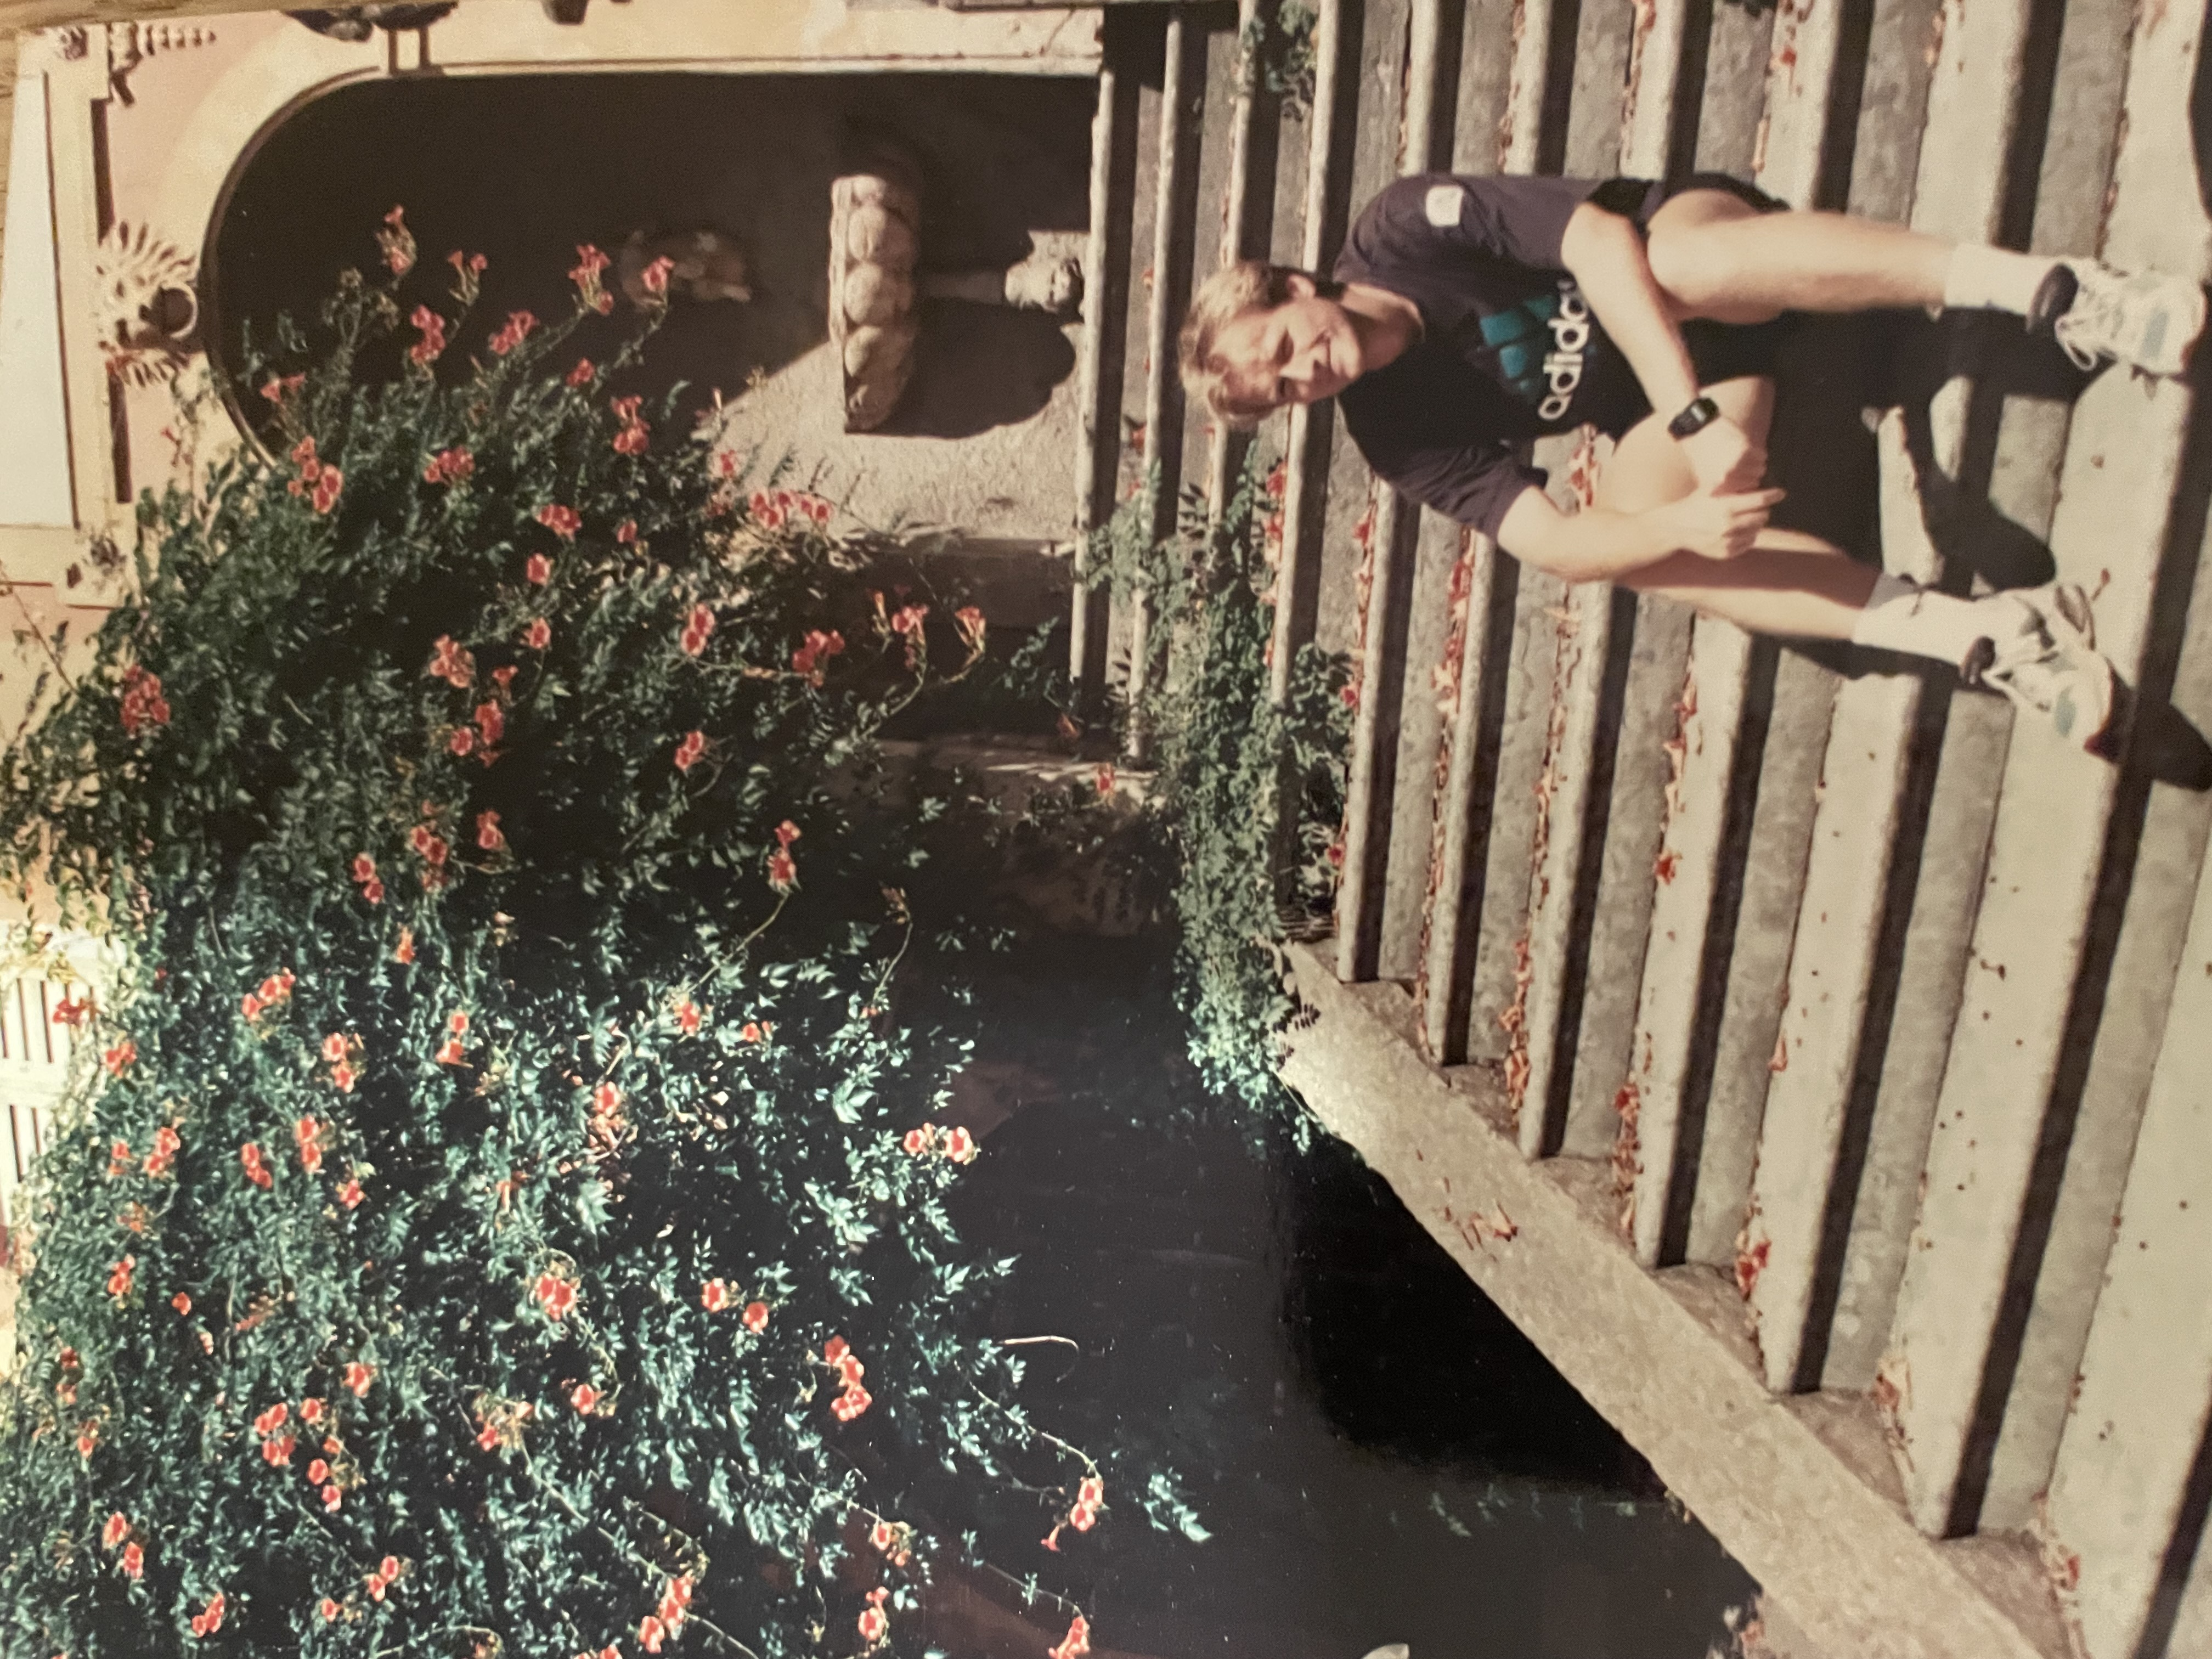
\includegraphics[width=0.8\linewidth]{Photos/mhj1995.jpeg}}

\vspace{6mm}
\end{frame}

\begin{frame}[plain,fragile]
\frametitle{Quantum computing, Overview and Motivation}

\textbf{How to use many-body theory to design quantum circuits (Quantum engineering)}
\begin{enumerate}
\item Many-body methods like F(ull)C(onfiguration)I(nteraction) theory  with
\begin{itemize}

  \item Adaptive basis sets (see for example \href{{https://arxiv.org/abs/2111.09638}}{Sigmundson et al arXiv:2111.09638})

  \item Time dependence

  \item Optimization of experimental parameter 

  \item Feedback from experiment

\end{itemize}

\noindent
\item Finding optimal parameters for tuning of entanglement

\item Numerical experiments to mimick real systems, using many-body methods to develop \textbf{quantum twins} (\href{{https://iopscience.iop.org/article/10.1088/1367-2630/12/7/075008}}{inspiration from  work by Herschel Rabitz et al on Control of quantum phenomena, see New Journal of Physics 12 (2010) 075008})!
\end{enumerate}

\noindent
\end{frame}

\begin{frame}[plain,fragile]
\frametitle{What is this about?}

Here we describe a method for generating motional entanglement between
two electrons trapped above the surface of superfluid helium. In this
proposed scheme these electronic charge qubits are laterally confined
via electrostatic gates to create an anharmonic trapping
potential. When the system is cooled to sufficiently low temperature
these in-plane charge qubit states are quantized and circuit quantum
electrodynamic methods can be used to control and readout single qubit
operations. Perspectives for quantum simulations with quantum dots
systems will be discussed.
\end{frame}

\begin{frame}[plain,fragile]
\frametitle{Literature and more reading}

\begin{enumerate}
\item \href{{https://journals.aps.org/rmp/abstract/10.1103/RevModPhys.95.011006}}{Justyna P. Zwolak and Jacob M. Taylor, Rev. Mod. Phys. 95, 011006, Advances in automation of quantum dot devices control}

\item \href{{https://arxiv.org/pdf/2210.14757.pdf}}{Pollanen and many other, Accelerating Progress Towards Practical Quantum Advantage: The Quantum Technology Demonstration Project Roadmap}

\item \href{{https://link.springer.com/book/10.1007/978-981-19-4641-7}}{Osada et al, introduction to quantum technologies, Springer, 2022}

\item \href{{https://journals.aps.org/pra/pdf/10.1103/PhysRevA.57.120}}{Original inspiration a series of articles of Loss and DiVincenzo from the nineties, Quantum Computation with Quantum Dots}
\end{enumerate}

\noindent
\end{frame}

\begin{frame}[plain,fragile]
\frametitle{Quantum Engineering}

\begin{block}{Quantum computing requirements }
\begin{enumerate}
\item be scalable

\item have qubits that can be entangled

\item have reliable initializations protocols to a standard state

\item have a set of universal quantum gates to control the quantum evolution

\item have a coherence time much longer than the gate operation time

\item have a reliable read-out mechanism for measuring the qubit states

\item ...more
\end{enumerate}

\noindent
\end{block}
\end{frame}

\begin{frame}[plain,fragile]
\frametitle{Candidate systems}

\begin{block}{}
\begin{enumerate}
\item Superconducting Josephon junctions

\item Single photons

\item \href{{https://journals.aps.org/rmp/pdf/10.1103/RevModPhys.93.025001}}{Trapped ions and atoms}

\item Nuclear Magnetic Resonance

\item \textbf{Quantum dots, experiments at MSU}

\item Point Defects in semiconductors

\item ...more
\end{enumerate}

\noindent
\end{block}
\end{frame}

\begin{frame}[plain,fragile]
\frametitle{Electrons (quantum dots) on superfluid helium}

Electrons on \textbf{superfluid helium represent} (see \href{{https://www.youtube.com/watch?v=EuDuM-fe-lA&ab_channel=JoshuahHeath}}{\nolinkurl{https://www.youtube.com/watch?v=EuDuM-fe-lA&ab_channel=JoshuahHeath}}) a promising platform for investigating
strongly-coupled qubits.

A systematic investigation of the
controlled generation of entanglement between two trapped electrons
under the influence of coherent microwave driving pulses, taking into
account the effects of the Coulomb interaction between electrons, may be of great interest for quantum information processing using
trapped electrons.
\end{frame}

\begin{frame}[plain,fragile]
\frametitle{To read more}

\begin{enumerate}
\item See \href{{https://www.nature.com/articles/s41586-022-04539-x}}{Single electrons on solid neon as a solid-state qubit platform, David Schuster et al, Nature \textbf{605}, 46–50 (2022)}

\item See Mark Dykman et al, Spin dynamics in quantum dots on liquid helium, PRB \textbf{107}. 035437 (2023) at \href{{https://link.aps.org/doi/10.1103/PhysRevB.107.035437}}{\nolinkurl{https://link.aps.org/doi/10.1103/PhysRevB.107.035437}}.
\end{enumerate}

\noindent
\end{frame}

\begin{frame}[plain,fragile]
\frametitle{Experimental setup I}

\vspace{6mm}

% inline figure
\centerline{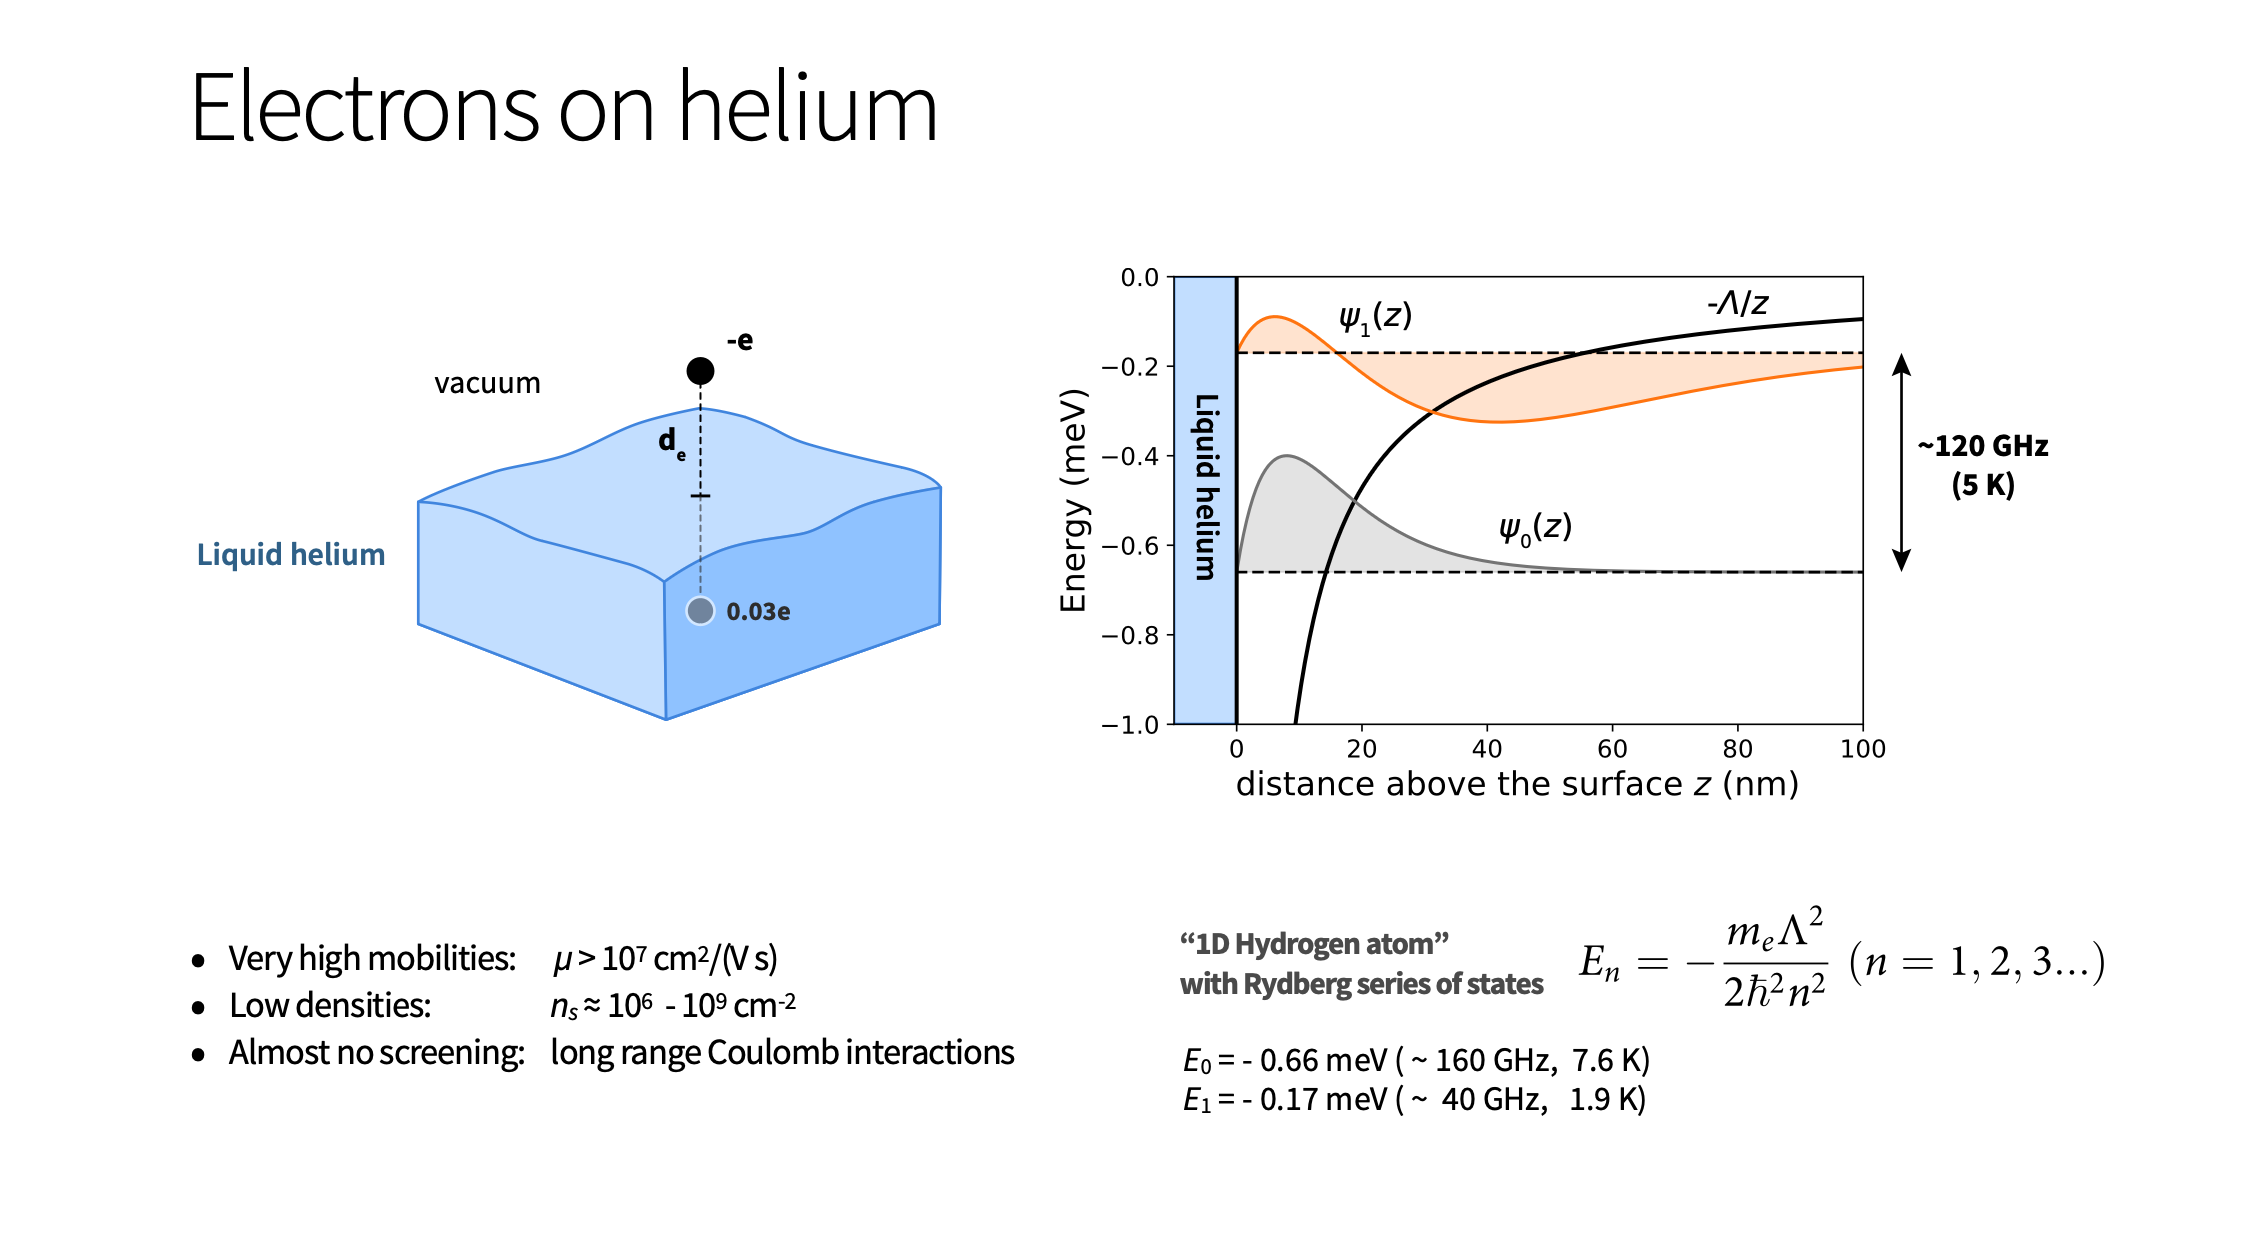
\includegraphics[width=1.3\linewidth]{qcfigures/Elhelium1.png}}

\vspace{6mm}
\end{frame}

\begin{frame}[plain,fragile]
\frametitle{More on experimental setup II}

\vspace{6mm}

% inline figure
\centerline{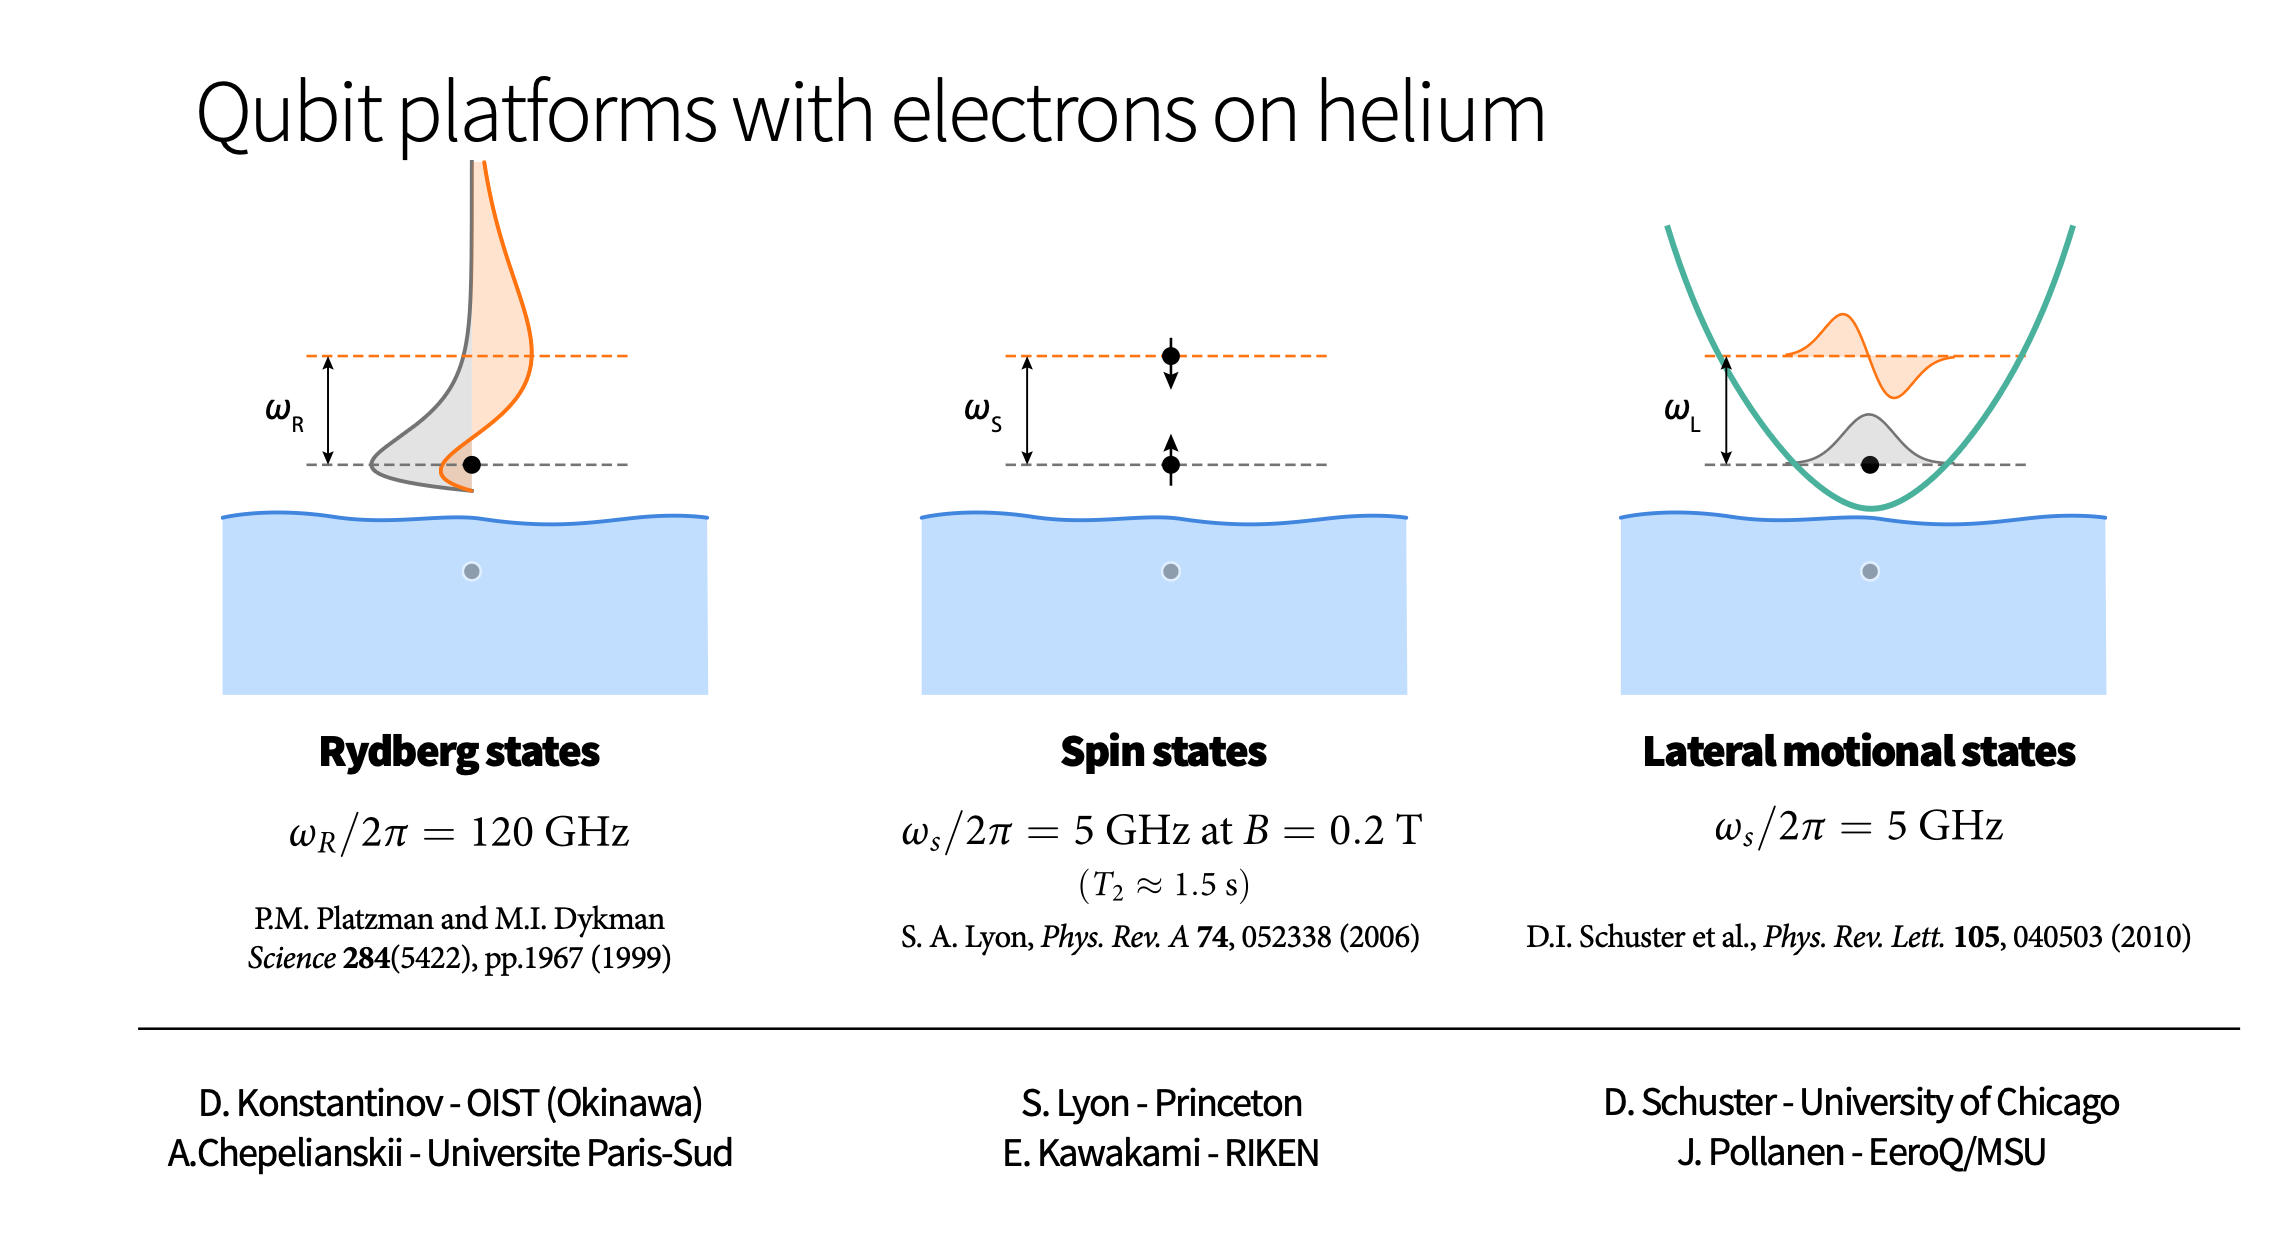
\includegraphics[width=1.3\linewidth]{qcfigures/Elhelium2.png}}

\vspace{6mm}
\end{frame}

\begin{frame}[plain,fragile]
\frametitle{More on experimental setup III}

\vspace{6mm}

% inline figure
\centerline{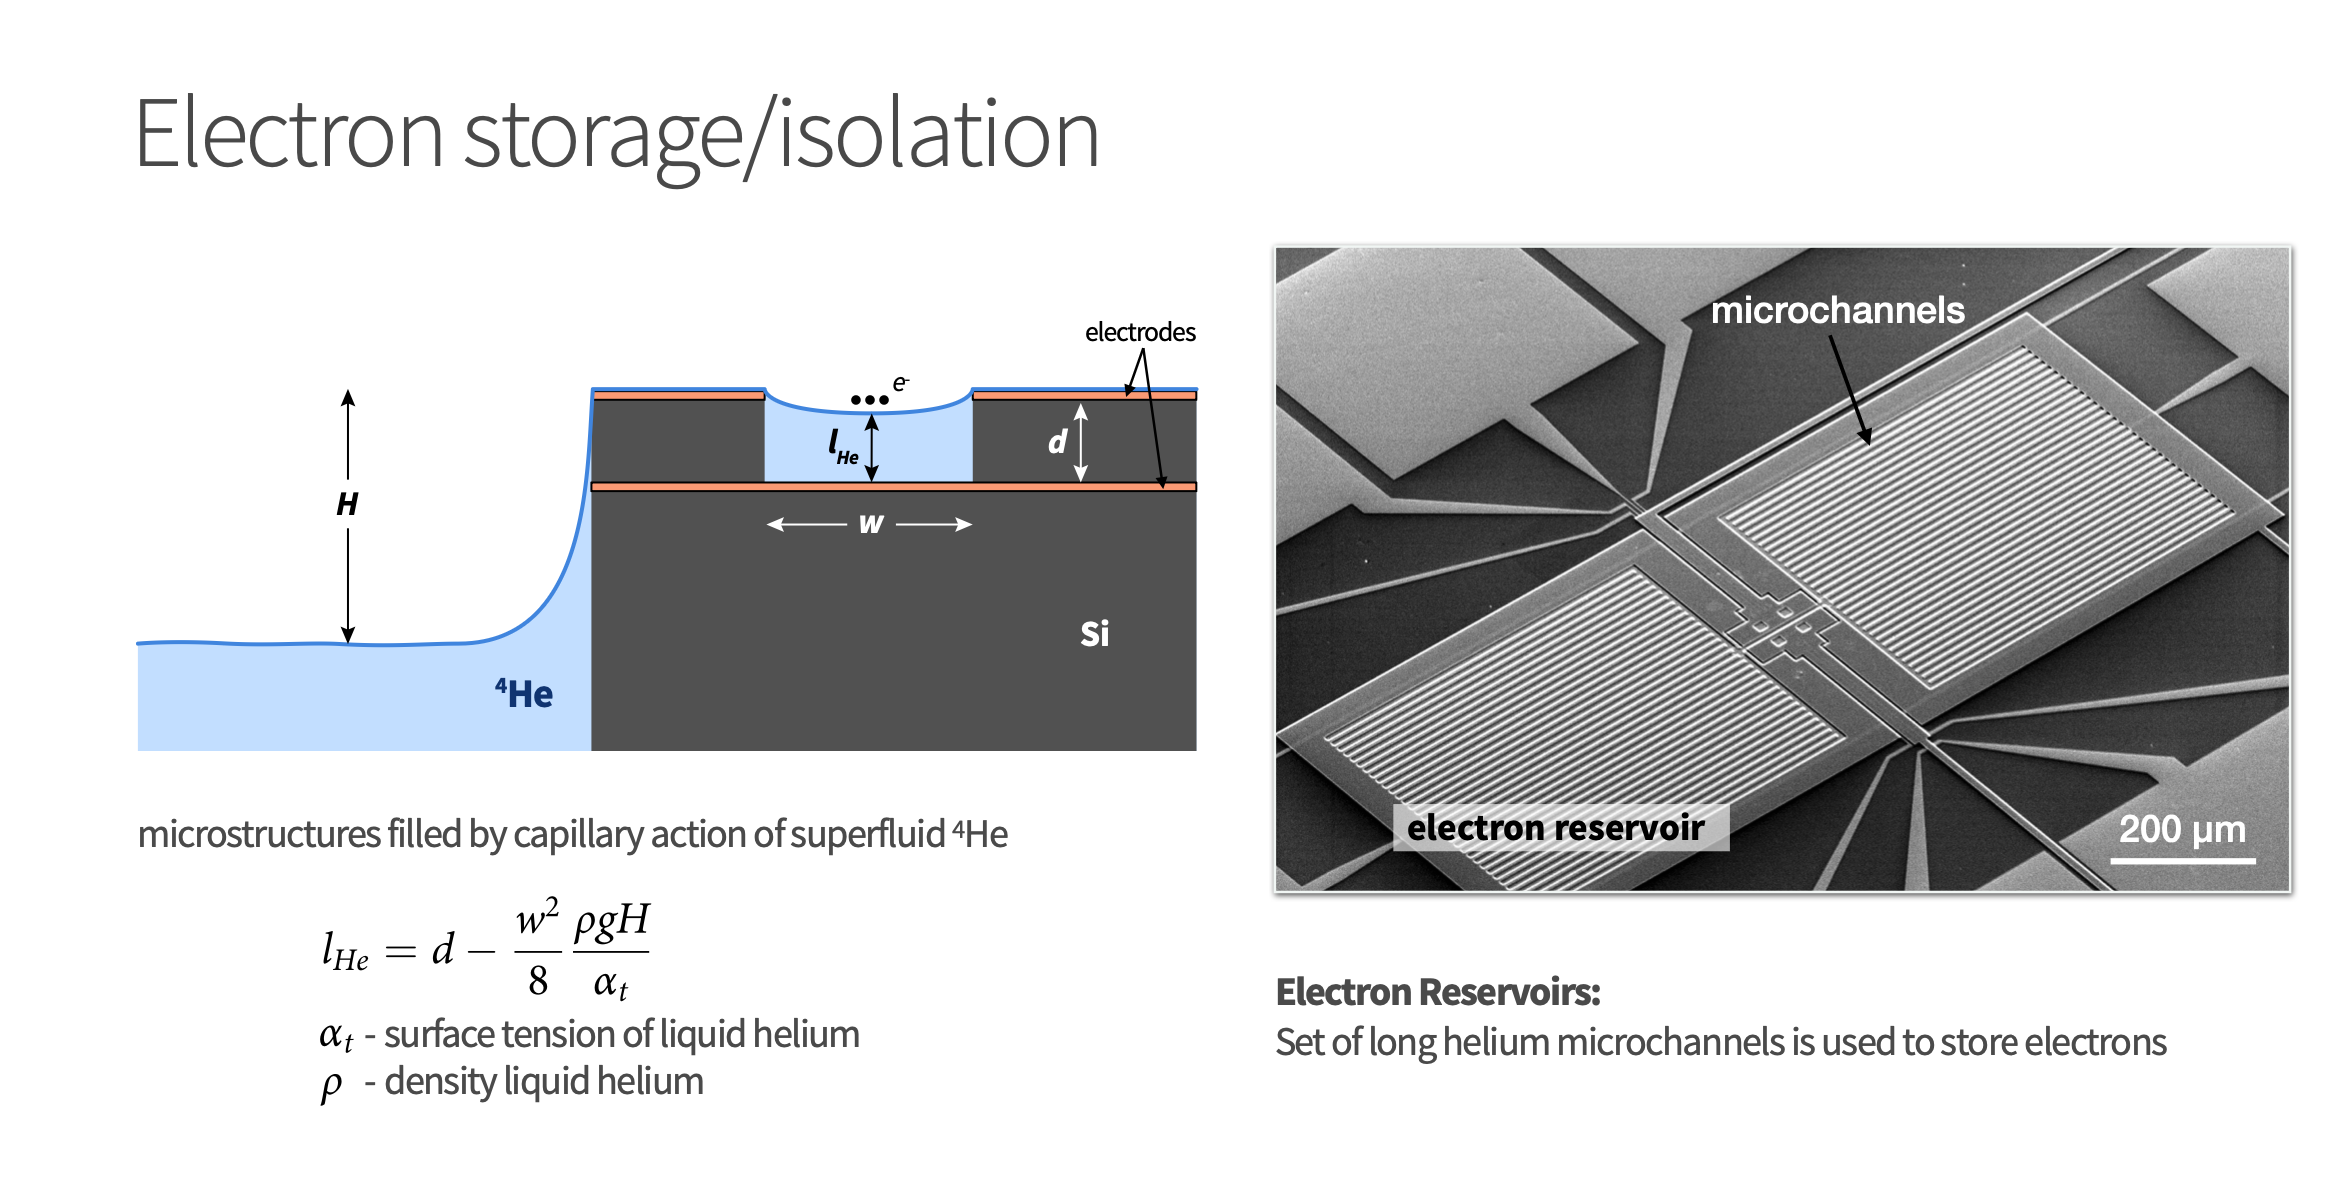
\includegraphics[width=1.3\linewidth]{qcfigures/Elhelium3.png}}

\vspace{6mm}
\end{frame}

\begin{frame}[plain,fragile]
\frametitle{Experimental set up}

\vspace{6mm}

% inline figure
\centerline{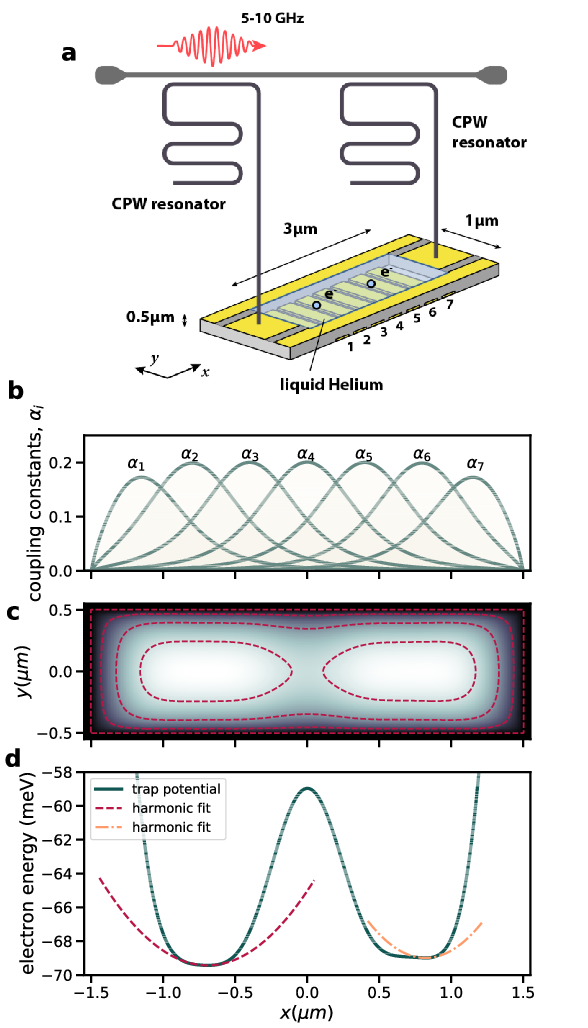
\includegraphics[width=0.7\linewidth]{qcfigures/figure1.png}}

\vspace{6mm}

\begin{enumerate}
\item (a) Schematic of the microdevice, where two electrons are trapped in a double-well potential created by electrodes 1-7. The read-out is provided by two superconducting resonators dispersively coupled to  electron's in-plane motional states.

\item (b) Coupling constants from each individual electrode beneath the helium layer.

\item (c+d) The electron's energy in a  double-well electrostatic potential (solid line). Dashed and dot-dashed lines represent the harmonic approximations of left and right wells respectively.
\end{enumerate}

\noindent
\end{frame}

\begin{frame}[plain,fragile]
\frametitle{Entanglement}

\begin{block}{}
\href{{https://link.springer.com/content/pdf/10.1007/s11232-007-0098-9.pdf}}{Entanglement} is the fundamental characteristic that distinguishes
quantum systems composed of two or more coupled objects from their
classical counterparts. The study of entanglement in precisely
engineered quantum systems with countably many degrees of freedom is
at the forefront of modern physics and is a key resource in quantum
information science (QIS). This is particularly true in the
development of two-qubit logic for quantum computation.
\end{block}

\begin{block}{}
The
generation of two-qubit entanglement has been demonstrated in a wide
variety of physical systems used in present-day quantum computing,
including superconducting circuits, trapped
ions, semiconductor quantum dots, color-center
defects in diamond, and neutral atoms in optical
lattices, just to name a few.
\end{block}
\end{frame}

\begin{frame}[plain,fragile]
\frametitle{More on Entanglement}

\begin{block}{}
Generating an entanglement between two quantum systems rely on
exploiting interactions in a controllable way. The details in the
interaction Hamiltonian between two systems defines the protocol
schemes for two-qubit logic.
\end{block}

\begin{block}{}
In  superconducting circuits the
interaction between qubits may arise from direct capacitive coupling
between circuit elements or by indirect coupling of two qubits to a
common resonator (virtually populating resonator mode) which results
in a non-local Hamiltonian in the form of exchange
interaction. This allow to implement various
schemes for entanglement, such as controlled-phase
gate, resonator-induced phase
gate, cross-resonance gates etc.
\end{block}
\end{frame}

\begin{frame}[plain,fragile]
\frametitle{Entanglement gates in trapped ions and more}

\begin{block}{}
Entanglement gates in trapped ions are
produced by means of the Coulomb interaction, where shared motional
modes of two or more ions, entangled to their internal states, used
for transferring excitations between ion
qubits. This has been experimentally
demonstrated.
\end{block}

\begin{block}{}
In photonic quantum
computing schemes two-qubit entangling operations are realized by
nonlinear interactions between two photons scattering from quantum
dots, plasmonic nanowires, diamond vacancy centers and others embedded
into waveguides. Two-qubit gates in
semiconductor quantum dots are based on spin-spin exchange
interactions or generated
by coupling to a superconducting resonator via artificial spin-orbit
interaction.
\end{block}
\end{frame}

\begin{frame}[plain,fragile]
\frametitle{Quantum dots and the Coulomb interaction}

\begin{block}{}
Coulomb interaction governed entanglement can be realized in
the system of electrons on the surface of superfluid helium, where
qubit states are formed by in-plane lateral motional or out-of plane
Rydberg states. Trapped near the surface of liquid helium these states
have different spatial charge configurations and the wavefunctions of
different electrons do not overlap.
\end{block}

\begin{block}{}
This results in a strong exchange
free Coulomb interaction which depends on the states of the
electrons. The lack of disorder in the systems
also leads to slow electron decoherence, which has attracted interest
to the system as a candidate for quantum information
processing.
\end{block}
\end{frame}

\begin{frame}[plain,fragile]
\frametitle{Electrons on helium is another qubit platform}

\textbf{To our knowledge two qubit gates have never been discussed in a proper manner for these systems.}

\begin{block}{}
The static Coulomb interaction arises from a virtual photon exchange
 process between two charge particles according to quantum
 electrodynamics. This results in a correlated motion of two charges
 generating quantum entanglement. 
\end{block}
\end{frame}

\begin{frame}[plain,fragile]
\frametitle{Surface state electrons (SSE)}

\begin{block}{}
Surface state electrons (SSE) 'floating' above liquid helium
originates from quantization of electron's perpendicular to the
surface motion in a trapping potential formed by attractive force from
image charge and a large $\sim$ 1 eV barrier at the liquid-vacuum
interface. At low temperatures the SSE are trapped in the lowest
Rydberg state for vertical motion some 11 nm above the helium surface,
which is perfectly clean and has a permittivity close to that of
vacuum.
\end{block}

\begin{block}{}
The weak interaction with rthe enviroment, which is mainly governed
by interaction with quantized surface capillary waves (ripplons) and
bulk phonons, ensures long coherence times - a vital ingredient for
any qubit platform. 
\end{block}
\end{frame}

\begin{frame}[plain,fragile]
\frametitle{Calculational details}

Hamiltonian:
\begin{align}
\hat{H} &=\frac{\hat{p}_1^2}{2} + \sum_{i = 1}^7 V_i\alpha_i[\hat{x}_1] + \frac{\hat{p}_2^2}{2} + \sum_{i = 1}^7 V_i\alpha_i[\hat{x}_2] + \frac{\kappa}{\sqrt{(\hat{x}_1-\hat{x}_2)^2 + a^2}}\\
&= h[\hat{p}_1,\hat{x}_1] + h[\hat{p}_2,\hat{x}_2] + u[\hat{x}_1,\hat{x}_2]
\end{align}

\vspace{6mm}

% inline figure
\centerline{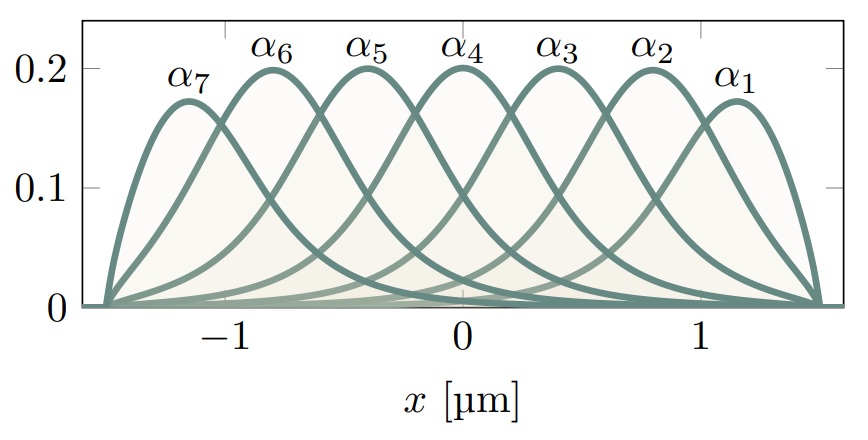
\includegraphics[width=0.8\linewidth]{qcfigures/well_basis.png}}

\vspace{6mm}
\end{frame}

\begin{frame}[plain,fragile]
\frametitle{Calculational details}

Hamiltonian:
\begin{align}
\hat{H} &= \frac{\hat{p}_1^2}{2} + v[\hat{x}_1] + \frac{\hat{p}_2^2}{2} + v[\hat{x}_2] + \frac{\kappa}{\sqrt{(\hat{x}_1-\hat{x}_2)^2 + a^2}}\\
&= h[\hat{p}_1,\hat{x}_1] + h[\hat{p}_2,\hat{x}_2] + u[\hat{x}_1,\hat{x}_2]
\end{align}

\vspace{6mm}

% inline figure
\centerline{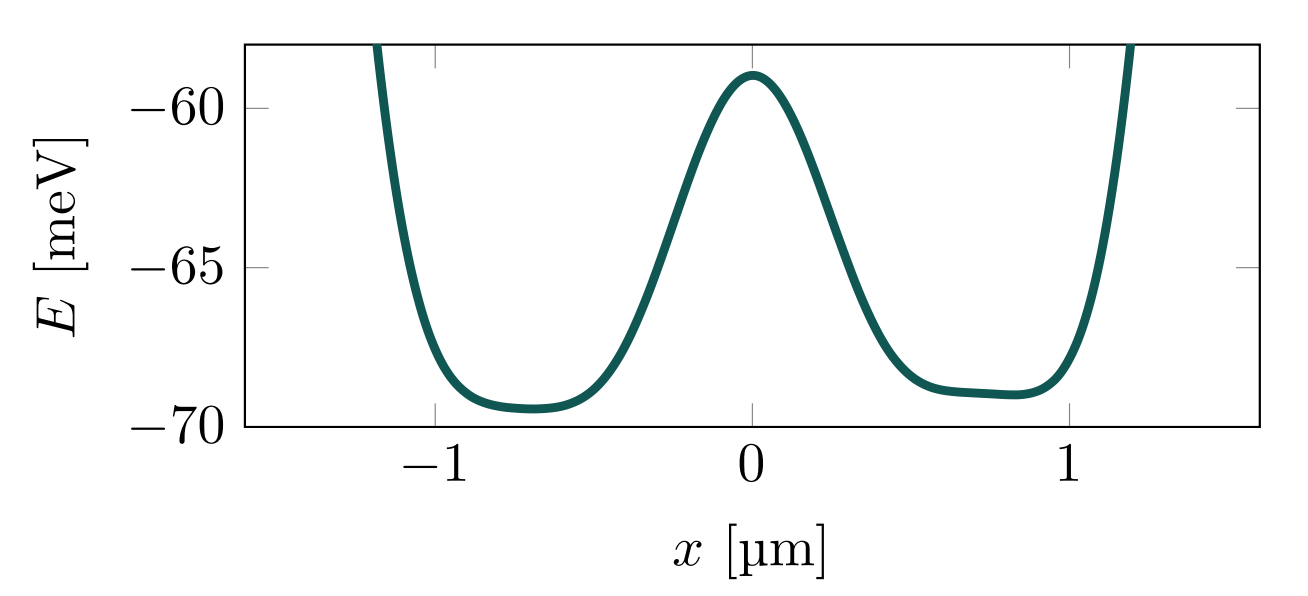
\includegraphics[width=0.8\linewidth]{qcfigures/wells.png}}

\vspace{6mm}
\end{frame}

\begin{frame}[plain,fragile]
\frametitle{Calculational details}

Hamiltonian:
\begin{align}
\hat{H} &= \frac{\hat{p}_1^2}{2} + v[\hat{x}_1] + \frac{\hat{p}_2^2}{2} + v[\hat{x}_2] + \frac{\kappa}{\sqrt{(\hat{x}_1-\hat{x}_2)^2 + a^2}} \\
&\equiv h[\hat{p}_1,\hat{x}_1] + h[\hat{p}_2,\hat{x}_2] + u[\hat{x}_1,\hat{x}_2]
\end{align}

Energy states:
\begin{equation}
\vert\Phi_k\rangle = \sum_{i < j} C_{ij, k}\frac{\vert \varphi_i \varphi_j\rangle - \vert \varphi_j \varphi_i\rangle}{\sqrt{2}},
\end{equation}
(Slater basis)
\end{frame}

\begin{frame}[plain,fragile]
\frametitle{Calculational details}

Hamiltonian:
\begin{align}
\hat{H} &= \frac{\hat{p}_1^2}{2} + v^L[\hat{x}_1] + \frac{\hat{p}_2^2}{2} + v^R[\hat{x}_2] + \frac{\kappa}{\sqrt{(\hat{x}_1-\hat{x}_2)^2 + a^2}} \\
&\equiv h^L[\hat{p}_1,\hat{x}_1] + h^R[\hat{p}_2,\hat{x}_2] + u[\hat{x}_1,\hat{x}_2]
\end{align}

Energy states:
\begin{equation}
\vert\Phi_k\rangle = \sum_{i} \sum_{j} C_{ij, k}\vert \varphi^L_i \varphi^R_j\rangle,
\end{equation}
(product basis)
\end{frame}

\begin{frame}[plain,fragile]
\frametitle{Calculational details}

Energy states:
\begin{equation}
\vert\Phi_k\rangle = \sum_{i} \sum_{j} C_{ij, k}\vert \varphi^L_i \varphi^R_j\rangle,
\end{equation}
(product basis)

\vspace{6mm}

% inline figure
\centerline{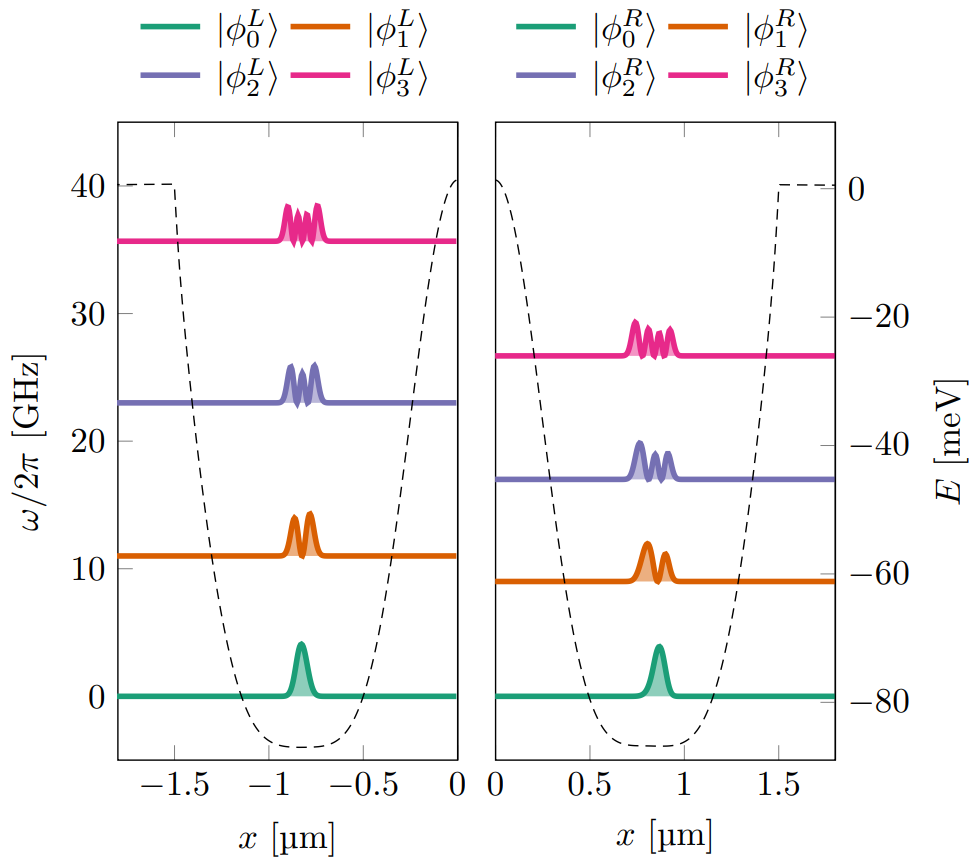
\includegraphics[width=0.9\linewidth]{qcfigures/Hartree_states.png}}

\vspace{6mm}
\end{frame}

\begin{frame}[plain,fragile]
\frametitle{Calculational details}

Hamiltonian:
\begin{align}
\hat{H} &= \frac{\hat{p}_1^2}{2} + v^L[\hat{x}_1] + \frac{\hat{p}_2^2}{2} + v^R[\hat{x}_2] + \frac{\kappa}{\sqrt{(\hat{x}_1-\hat{x}_2)^2 + a^2}} \\
&\equiv h^L[\hat{p}_1,\hat{x}_1] + h^R[\hat{p}_2,\hat{x}_2] + u[\hat{x}_1,\hat{x}_2]
\end{align}

Energy states:
\begin{equation}
\vert\Phi_k\rangle = \sum_{i} \sum_{j} C_{ij, k}\vert \varphi^L_i \varphi^R_j\rangle,
\end{equation}
(Hartree basis)
\end{frame}

\begin{frame}[plain,fragile]
\frametitle{Calculational details}

Hamiltonian:
\begin{align}
\hat{H} &= \frac{\hat{p}_1^2}{2} + v^L[\hat{x}_1] + \frac{\hat{p}_2^2}{2} + v^R[\hat{x}_2] + \frac{\kappa}{\sqrt{(\hat{x}_1-\hat{x}_2)^2 + a^2}} \\
&\equiv h^L[\hat{p}_1,\hat{x}_1] + h^R[\hat{p}_2,\hat{x}_2] + u[\hat{x}_1,\hat{x}_2]
\end{align}

Energy states:
\begin{equation}
\vert\Phi_k\rangle = \sum_{i = 0}^{N^L} \sum_{j = 0}^{N^R} C_{ij, k}\vert \varphi^L_i \varphi^R_j\rangle,
\end{equation}
(Hartree basis)
\end{frame}

\begin{frame}[plain,fragile]
\frametitle{Calculational details}

Energy states:
\begin{equation}
\vert\Phi_k\rangle = \sum_{i = 0}^{N^L} \sum_{j = 0}^{N^R} C_{ij, k}\vert \varphi^L_i \varphi^R_j\rangle,
\end{equation}
(Hartree basis)

\vspace{6mm}

% inline figure
\centerline{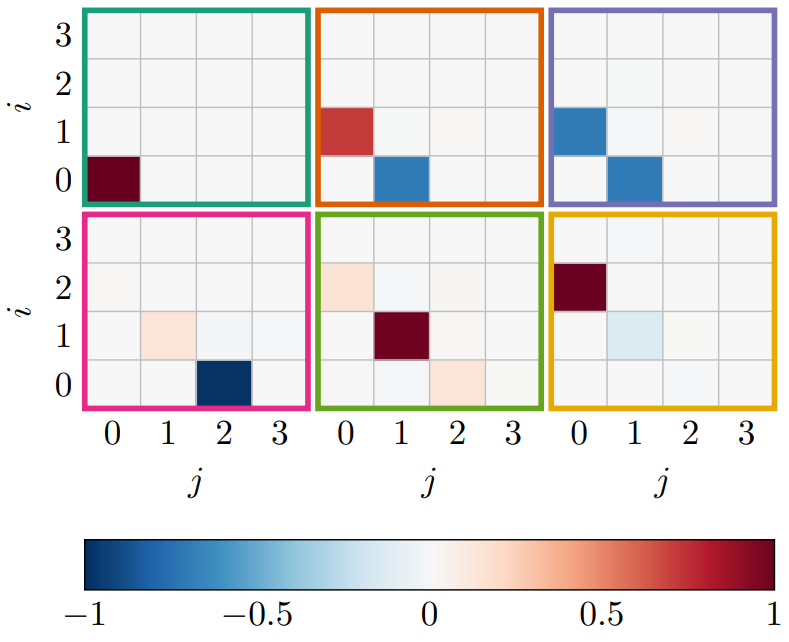
\includegraphics[width=0.7\linewidth]{qcfigures/Hartree_coefs.png}}

\vspace{6mm}
\end{frame}

\begin{frame}[plain,fragile]
\frametitle{Calculational details}

Hamiltonian:
\begin{align}
\hat{H} &= \frac{\hat{p}_1^2}{2} + v^L[\hat{x}_1] + \frac{\hat{p}_2^2}{2} + v^R[\hat{x}_2] + \frac{\kappa}{\sqrt{(\hat{x}_1-\hat{x}_2)^2 + a^2}} \\
&\equiv h^L[\hat{p}_1,\hat{x}_1] + h^R[\hat{p}_2,\hat{x}_2] + u[\hat{x}_1,\hat{x}_2]
\end{align}

Energy states:
\begin{equation}
\vert\Phi_k\rangle = \sum_{i = 0}^{N^L} \sum_{j = 0}^{N^R} C_{ij, k}\vert \varphi^L_i \varphi^R_j\rangle,
\end{equation}
(Hartree basis)
\end{frame}

\begin{frame}[plain,fragile]
\frametitle{Results and discussions}

By adjusting the potential we can change the anharmonicities and detuning of the wells.
\begin{enumerate}
\item What values of these give interesting interactions?

\item Inspiration from superconducting qubits, see High-Contrast $ZZ$ Interaction Using Superconducting Qubits with Opposite-Sign Anharmonicity, \href{{https://journals.aps.org/prl/abstract/10.1103/PhysRevLett.125.200503}}{Zhao et al Phys. Rev. Lett. 125, 200503}
\end{enumerate}

\noindent
\end{frame}

\begin{frame}[plain,fragile]
% No title on this slide

We search for well configurations corresponding to three different types of interaction between the two electrons.

\begin{enumerate}
\item In configuration I we address both qubits independently and can thereby perform single-qubit state rotations and measurements.

\item Configurations II and III correspond to avoided level crossings between two ($E_{01}, E_{10}$) and three ($E_{11}, E_{20}, E_{02}$) energy levels respectively, where the electrons' motion becomes correlated, that is they are entangled. 
\end{enumerate}

\noindent
Both anharmonicity and detuning changes with the shape of our well.
We create a voltage parameterization
\begin{equation}
V(\lambda) = (1-\lambda)V_\mathrm{I} + \lambda V_\mathrm{III}
\end{equation}
\end{frame}

\begin{frame}[plain,fragile]
\frametitle{Entanglement and more}

\vspace{6mm}

% inline figure
\centerline{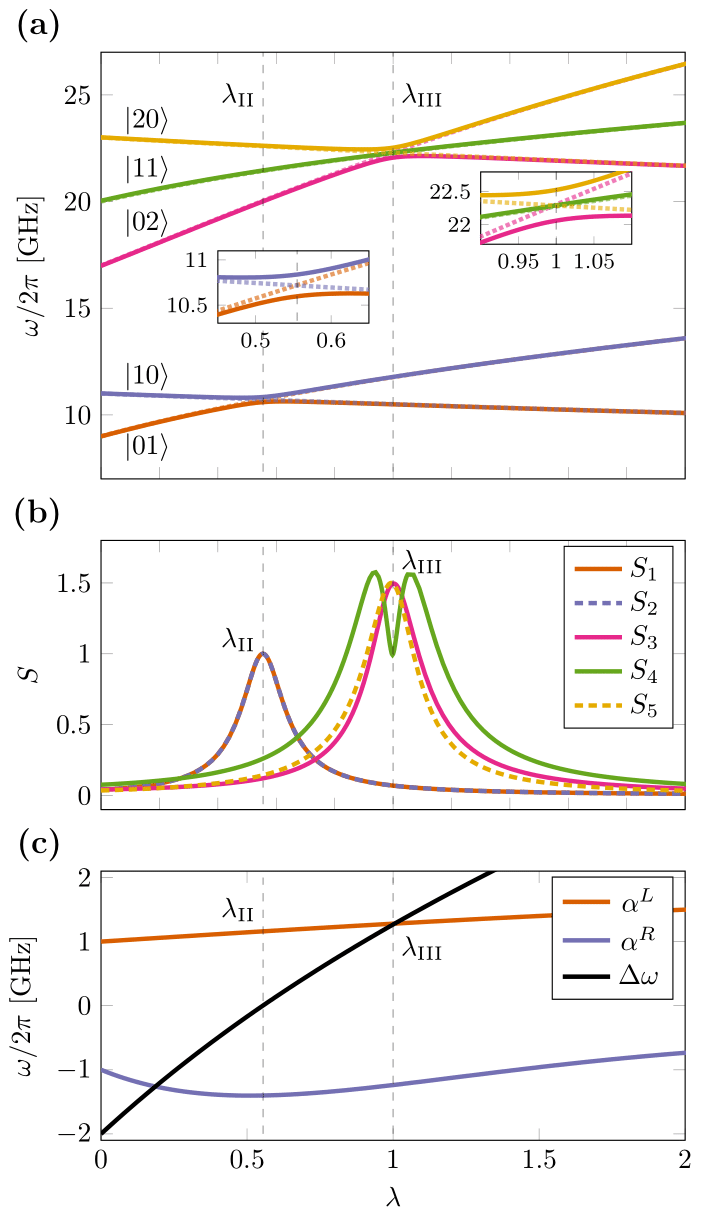
\includegraphics[width=0.7\linewidth]{qcfigures/crossings-entropies-anharmonicities-1.png}}

\vspace{6mm}
\end{frame}

\begin{frame}[plain,fragile]
\frametitle{Legend to figure}

\begin{enumerate}
\item (a) In this figure we have plotted the transition energy from the ground state to the labeled excited state as a function of the voltage parameter $\lambda$. The labeled states are the computational basis states when $\lambda = 0$.

\item (b) The von Neumann entropy of the five lowest excited states of the two-body Hamiltonian as a function of the configuration parameter $\lambda$. The ground state has zero entropy, or close to zero entropy. We have included the points for the double and triple degeneracy points. $\lambda_{II}$ and $\lambda_{III}$ in the figure. The von Neumann entropy is calculated using the binary logarithm.

\item (c) In this figure we have plotted the anharmonicites for the left well ($\alpha^L$) and the right well ($\alpha^R$) as a function of the well parameterization $\lambda$. We have also included the detuning $\Delta \omega = \omega^R - \omega^L$ between the two wells. We have marked configuration II at $\lambda_{II} \approx 0.554$ and configuration III at $\lambda_{III} = 1$.
\end{enumerate}

\noindent
\end{frame}

\begin{frame}[plain,fragile]
\frametitle{Particle densities and coefficients}

\vspace{6mm}

% inline figure
\centerline{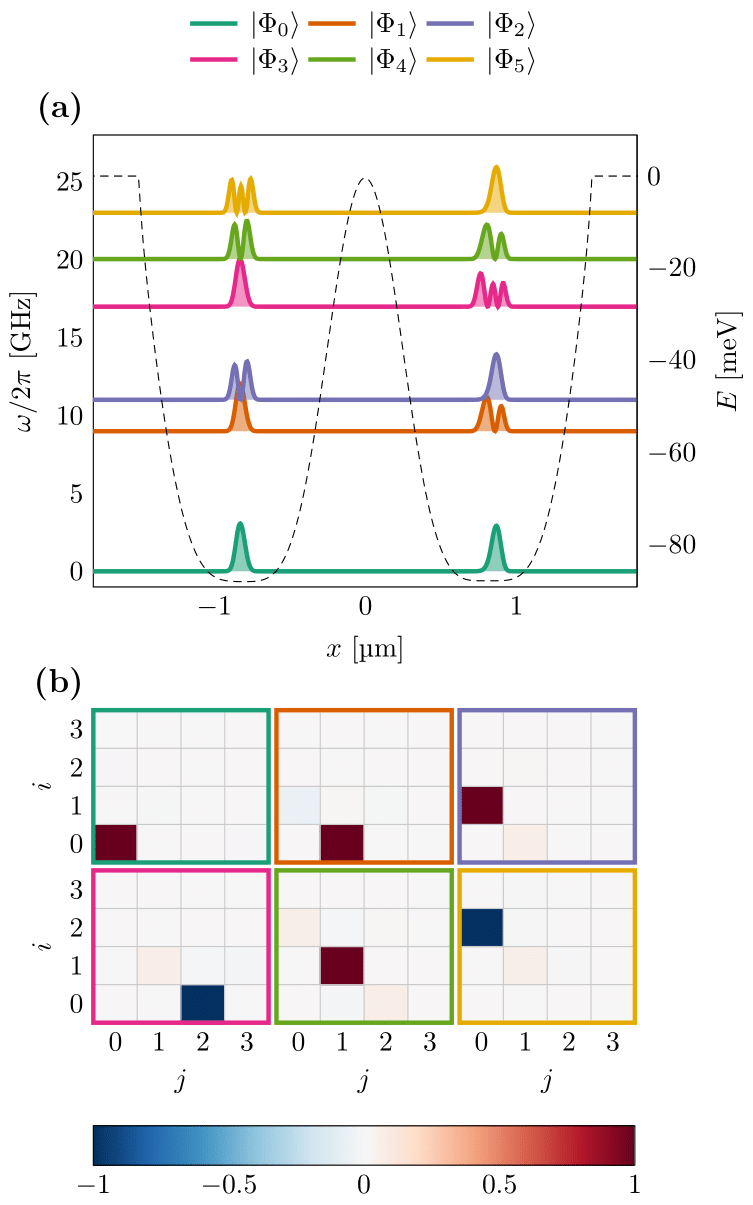
\includegraphics[width=0.7\linewidth]{qcfigures/configuration_I-1.png}}

\vspace{6mm}
\end{frame}

\begin{frame}[plain,fragile]
\frametitle{Potential wells, the one-body densities, and single-particle states}

\vspace{6mm}

% inline figure
\centerline{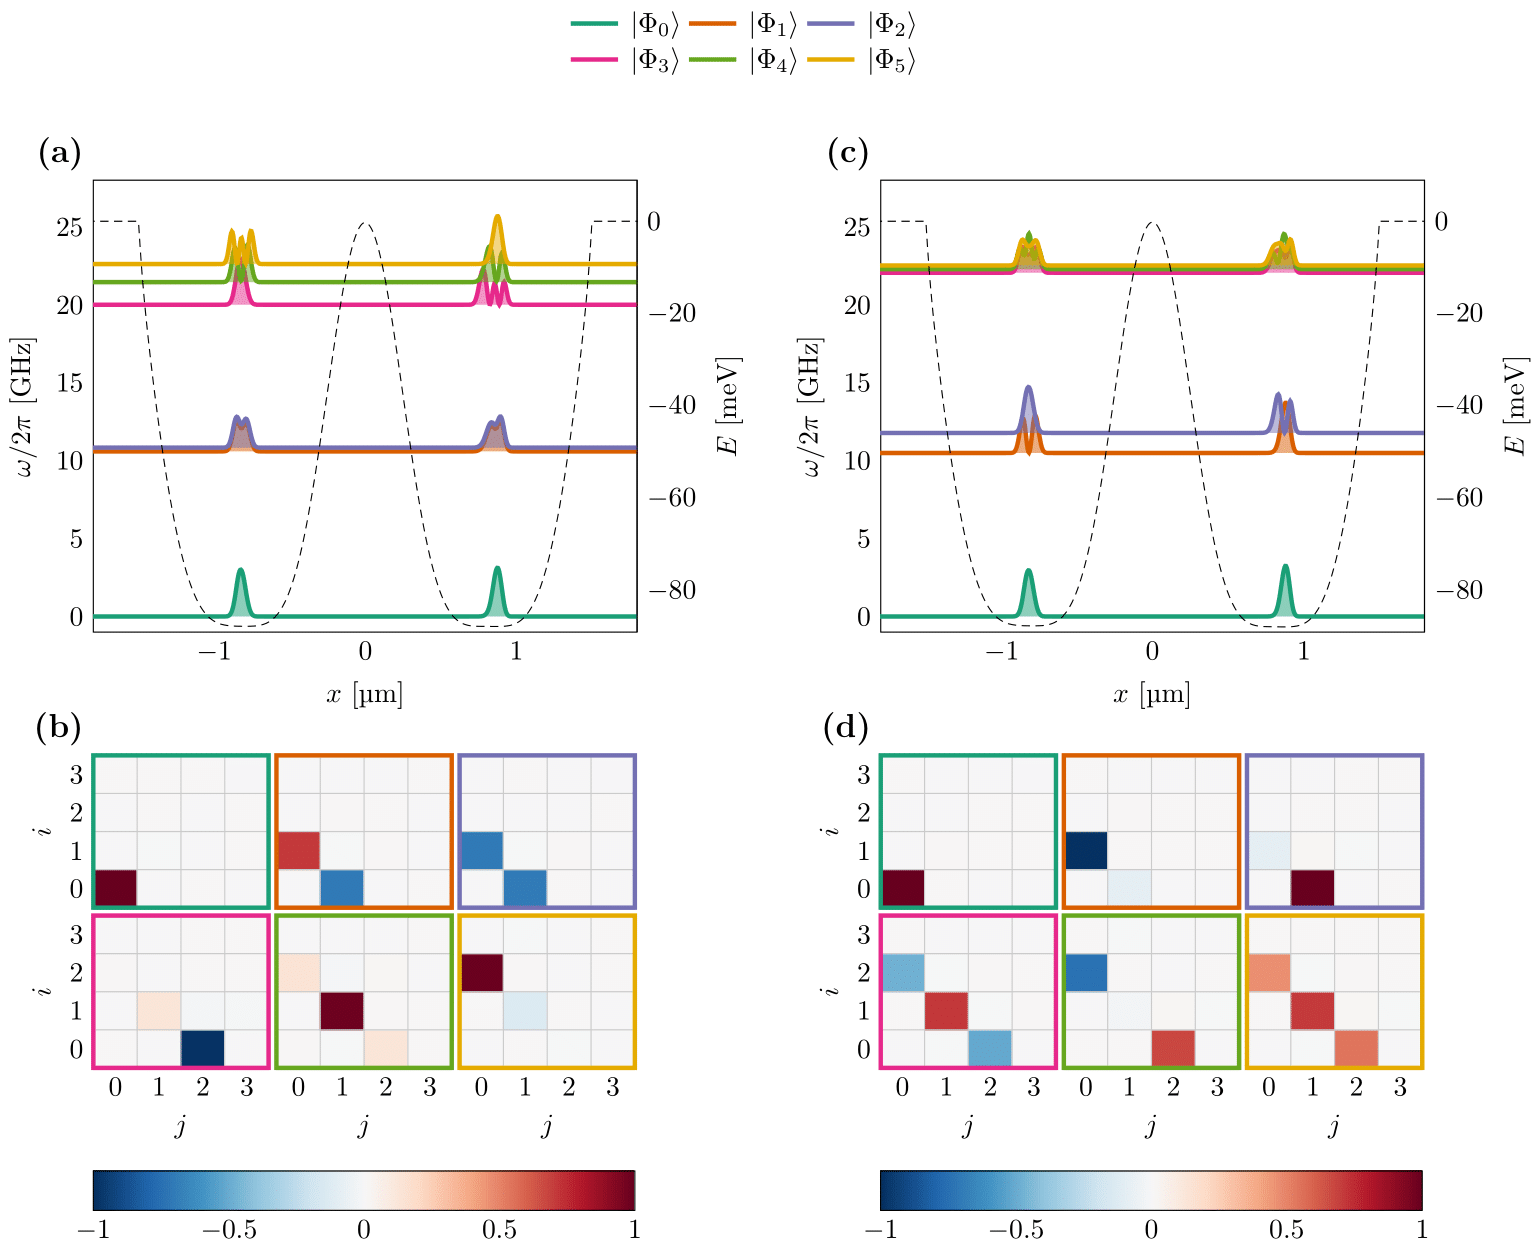
\includegraphics[width=0.7\linewidth]{qcfigures/configuration_II_and_III-1.png}}

\vspace{6mm}
\end{frame}

\begin{frame}[plain,fragile]
\frametitle{Where we are now}

\begin{enumerate}
\item Adding time-dependent studies of two electrons in two wells in one and two dimensions

\item Studies of the time-evolution of entangled states (now two electrons only)

\item Use theory to find optimal experimental setup

\item Expect two-electron system realized experimentally in approx $1$ year, great potential for studies of quantum simulations
\end{enumerate}

\noindent
\end{frame}

\begin{frame}[plain,fragile]
\frametitle{Plans}

\begin{enumerate}
\item Add two and three-dimensions in order to simulate in  a more realistic way such many-body systems.

\item Develop time-dependent FCI code, useful up to approximately 10 particles with \textbf{effective} (and effective Hilbert space) Hamiltonians in two and three dimensions

\item Develop codes for studies of entanglement as function of time

\item Do tomogrophy and extract density matrix and compare with experiment.

\item Study the feasibility of various setups for quantum simulations of specific Hamiltonians such as the Lipkin model

\item For larger many-body systems, study for example time-dependent CC theory
\end{enumerate}

\noindent
\end{frame}

\begin{frame}[plain,fragile]
\frametitle{Addendum: Quantum Monte Carlo Motivation}

\begin{block}{}
Given a hamiltonian $H$ and a trial wave function $\Psi_T$, the variational principle states that the expectation value of $\langle H \rangle$, defined through 
\[
   \langle E \rangle =
   \frac{\int d\bm{R}\Psi^{\ast}_T(\bm{R})H(\bm{R})\Psi_T(\bm{R})}
        {\int d\bm{R}\Psi^{\ast}_T(\bm{R})\Psi_T(\bm{R})},
\]
is an upper bound to the ground state energy $E_0$ of the hamiltonian $H$, that is 
\[
    E_0 \le \langle E \rangle.
\]
In general, the integrals involved in the calculation of various  expectation values  are multi-dimensional ones. Traditional integration methods such as the Gauss-Legendre will not be adequate for say the  computation of the energy of a many-body system.
\end{block}
\end{frame}

\begin{frame}[plain,fragile]
\frametitle{Quantum Monte Carlo Motivation}

\begin{block}{Basic steps }
Choose a trial wave function
$\psi_T(\bm{R})$.
\[
   P(\bm{R},\bm{\alpha})= \frac{\left|\psi_T(\bm{R},\bm{\alpha})\right|^2}{\int \left|\psi_T(\bm{R},\bm{\alpha})\right|^2d\bm{R}}.
\]
This is our model, or likelihood/probability distribution function  (PDF). It depends on some variational parameters $\bm{\alpha}$.
The approximation to the expectation value of the Hamiltonian is now 
\[
   \langle E[\bm{\alpha}] \rangle = 
   \frac{\int d\bm{R}\Psi^{\ast}_T(\bm{R},\bm{\alpha})H(\bm{R})\Psi_T(\bm{R},\bm{\alpha})}
        {\int d\bm{R}\Psi^{\ast}_T(\bm{R},\bm{\alpha})\Psi_T(\bm{R},\bm{\alpha})}.
\]
\end{block}
\end{frame}

\begin{frame}[plain,fragile]
\frametitle{Quantum Monte Carlo Motivation}

\begin{block}{Define a new quantity }
\[
   E_L(\bm{R},\bm{\alpha})=\frac{1}{\psi_T(\bm{R},\bm{\alpha})}H\psi_T(\bm{R},\bm{\alpha}),
\]
called the local energy, which, together with our trial PDF yields
\[
  \langle E[\bm{\alpha}] \rangle=\int P(\bm{R})E_L(\bm{R},\bm{\alpha}) d\bm{R}\approx \frac{1}{N}\sum_{i=1}^NE_L(\bm{R_i},\bm{\alpha})
\]
with $N$ being the number of Monte Carlo samples.
\end{block}
\end{frame}

\begin{frame}[plain,fragile]
\frametitle{The trial wave function}

\begin{block}{}
We want to perform  a Variational Monte Carlo calculation of the ground state of two electrons in a quantum dot well with different oscillator energies, assuming total spin $S=0$.
Our trial wave function has the following form
\begin{equation}
   \psi_{T}(\bm{r}_1,\bm{r}_2) = 
   C\exp{\left(-\alpha_1\omega(r_1^2+r_2^2)/2\right)}
   \exp{\left(\frac{r_{12}}{(1+\alpha_2 r_{12})}\right)}, 
\label{eq:trial}
\end{equation}
where the variables $\alpha_1$ and $\alpha_2$ represent our variational parameters.

Why does the trial function look like this? How did we get there? \textbf{This is one of our main motivations} for switching to
Machine Learning.

\end{block}
\end{frame}

\begin{frame}[plain,fragile]
\frametitle{The correlation part of the wave function}

To find an ansatz for the correlated part of the wave function, it is useful to rewrite the two-particle
local energy in terms of the relative and center-of-mass motion.
Let us denote the distance between the two electrons as
$r_{12}$. We omit the center-of-mass motion since we are only interested in the case when
$r_{12} \rightarrow 0$. The contribution from the center-of-mass (CoM) variable $\bm{R}_{\mathrm{CoM}}$
gives only a finite contribution.
We focus only on the terms that are relevant for $r_{12}$ and for three dimensions. The relevant local energy operator becomes then (with $l=0$)
\[
\lim_{r_{12} \rightarrow 0}E_L(R)=
    \frac{1}{{\cal R}_T(r_{12})}\left(-2\frac{d^2}{dr_{ij}^2}-\frac{4}{r_{ij}}\frac{d}{dr_{ij}}+
\frac{2}{r_{ij}}\right){\cal R}_T(r_{12}).
\]
In order to avoid divergencies when $r_{12}\rightarrow 0$ we obtain  the so-called \textbf{cusp} condition
\[
\frac{d {\cal R}_T(r_{12})}{dr_{12}} = \frac{1}{2}
{\cal R}_T(r_{12})\qquad r_{12}\to 0
\]
\end{frame}

\begin{frame}[plain,fragile]
\frametitle{Resulting ansatz}

The above  results in
\[
{\cal R}_T  \propto \exp{(r_{ij}/2)}, 
\]
for anti-parallel spins and 
\[
{\cal R}_T  \propto \exp{(r_{ij}/4)}, 
\]
for anti-parallel spins. 
This is the so-called cusp condition for the relative motion, resulting in a minimal requirement
for the correlation part of the wave fuction.
For general systems containing more than say two electrons, we have this
condition for each electron pair $ij$.
\end{frame}

\begin{frame}[plain,fragile]
\frametitle{Energy derivatives}

\begin{block}{}
To find the derivatives of the local energy expectation value as function of the variational parameters, we can use the chain rule and the hermiticity of the Hamiltonian.  

Let us define (with the notation $\langle E[\bm{\alpha}]\rangle =\langle  E_L\rangle$)
\[
\bar{E}_{\alpha_i}=\frac{d\langle  E_L\rangle}{d\alpha_i},
\]
as the derivative of the energy with respect to the variational parameter $\alpha_i$
We define also the derivative of the trial function (skipping the subindex $T$) as 
\[
\bar{\Psi}_{i}=\frac{d\Psi}{d\alpha_i}.
\]
\end{block}
\end{frame}

\begin{frame}[plain,fragile]
\frametitle{Derivatives of the local energy}

\begin{block}{}
The elements of the gradient of the local energy are then (using the chain rule and the hermiticity of the Hamiltonian)
\[
\bar{E}_{i}= 2\left( \langle \frac{\bar{\Psi}_{i}}{\Psi}E_L\rangle -\langle \frac{\bar{\Psi}_{i}}{\Psi}\rangle\langle E_L \rangle\right).
\]
From a computational point of view it means that you need to compute the expectation values of 
\[
\langle \frac{\bar{\Psi}_{i}}{\Psi}E_L\rangle,
\]
and
\[
\langle \frac{\bar{\Psi}_{i}}{\Psi}\rangle\langle E_L\rangle
\]
These integrals are evaluted using MC intergration (with all its possible error sources). 
We can then use methods like stochastic gradient or other minimization methods to find the optimal variational parameters (I don't discuss this topic here, but these methods are very important in ML). 
\end{block}
\end{frame}

\begin{frame}[plain,fragile]
\frametitle{How do we define our cost function?}

\begin{block}{}
We have a model, our likelihood function. 

How should we define the cost function?

\end{block}
\end{frame}

\begin{frame}[plain,fragile]
\frametitle{Meet the variance and its derivatives}

\begin{block}{Why the variance? }
Suppose the trial function (our model) is the exact wave function. The action of the hamiltionan
on the wave function
\[
   H\Psi = \mathrm{constant}\times \Psi,
\]
The integral which defines various 
expectation values involving moments of the hamiltonian becomes then
\[
   \langle E^n \rangle =   \langle H^n \rangle =
   \frac{\int d\bm{R}\Psi^{\ast}(\bm{R})H^n(\bm{R})\Psi(\bm{R})}
        {\int d\bm{R}\Psi^{\ast}(\bm{R})\Psi(\bm{R})}=
\mathrm{constant}\times\frac{\int d\bm{R}\Psi^{\ast}(\bm{R})\Psi(\bm{R})}
        {\int d\bm{R}\Psi^{\ast}(\bm{R})\Psi(\bm{R})}=\mathrm{constant}.
\]
\textbf{This gives an important information: If I want the variance, the exact wave function leads to zero variance!}
The variance is defined as 
\[
\sigma_E = \langle E^2\rangle - \langle E\rangle^2.
\]
Variation is then performed by minimizing both the energy and the variance.

\end{block}
\end{frame}

\begin{frame}[plain,fragile]
\frametitle{The variance defines the cost function}

\begin{block}{}
We can then take the derivatives of 
\[
\sigma_E = \langle E^2\rangle - \langle E\rangle^2,
\]
with respect to the variational parameters. The derivatives of the variance can then be used to defined the
so-called Hessian matrix, which in turn allows us to use minimization methods like Newton's method or 
standard gradient methods. 

This leads to however a more complicated expression, with obvious errors when evaluating integrals by Monte Carlo integration. Less used, see however \href{{https://journals.aps.org/prl/abstract/10.1103/PhysRevLett.94.150201}}{Filippi and Umrigar}. The expression becomes complicated
\begin{align}
\bar{E}_{ij} &= 2\left[ \langle (\frac{\bar{\Psi}_{ij}}{\Psi}+\frac{\bar{\Psi}_{j}}{\Psi}\frac{\bar{\Psi}_{i}}{\Psi})(E_L-\langle E\rangle)\rangle -\langle \frac{\bar{\Psi}_{i}}{\Psi}\rangle\bar{E}_j-\langle \frac{\bar{\Psi}_{j}}{\Psi}\rangle\bar{E}_i\right] \\ \nonumber
&+\langle \frac{\bar{\Psi}_{i}}{\Psi}E_L{_j}\rangle +\langle \frac{\bar{\Psi}_{j}}{\Psi}E_L{_i}\rangle -\langle \frac{\bar{\Psi}_{i}}{\Psi}\rangle\langle E_L{_j}\rangle \langle \frac{\bar{\Psi}_{j}}{\Psi}\rangle\langle E_L{_i}\rangle.  
\end{align}

Evaluating the cost function means having to evaluate the above second derivative of the energy. 

\end{block}
\end{frame}

\end{document}
